%\documentclass[a4paper]{article}
% #### CONFIGURACIONES ####
\documentclass[12pt,a4paper,oneside]{book} % tamaño 12
%\usepackage[spanish]{babel}
\usepackage[spanish, es-tabla]{babel}
\usepackage[utf8x]{inputenc}
\usepackage[pass]{geometry}
\usepackage[usenames]{color}
\usepackage[table,xcdraw]{xcolor}
\usepackage{tikz} % grafos
\usetikzlibrary{arrows,shapes,positioning,shadows,trees}
\usepackage{amsmath} % códigos
\usepackage{setspace} %interlineado algoritmo
\usepackage{algorithm}
%\usepackage{algorithmicx}
\usepackage{algpseudocode}
\usepackage{rotating} % rotate graphics
\usepackage{pdflscape} % automatic rotation of the page 
\usepackage{longtable}
\algdef{SE}[DOWHILE]{Do}{doWhile}{\algorithmicdo}[1]{\algorithmicwhile\ #1}%
\usepackage[hidelinks]{hyperref}
\usepackage{subfig} % Para poner imágenes
\usepackage{graphicx} % para poner dos imágenes juntas
\usepackage[colorinlistoftodos]{todonotes}
\usepackage{anysize}
\marginsize{4cm}{2.5cm}{2.5cm}{2.5cm}
% Márgenes {izquierda}{derecha}{arriba}{abajo}.
\usepackage{mathptmx}% http://ctan.org/pkg/mathptmx Times new roman
\usepackage{amsfonts}% Para expresiones matemáticas
%\usepackage{setspace} % interlineado
\renewcommand{\baselinestretch}{1.5} % Interlineado
\usepackage{enumerate}% para los enumerate
\usepackage{fancyhdr}
\pagestyle{fancy}
\usepackage[none]{hyphenat} %saltos y justificación texto
\usepackage{float}
\usepackage{tikz}
\usetikzlibrary{calc}
\usepackage{changepage}
\usepackage{ragged2e}
\usepackage{tabularx} % Para meter tablas que no excedan los márgenes del papel
\usepackage{fancyhdr}
%%%%%%%%%%%%%%%%%%%%%%%
%%%%%%%% XML %%%%%%%%%%
\usepackage{listings}

\usepackage{appendix}
% cambiar apéndices por anexos
\renewcommand{\appendixname}{Anexos}
\renewcommand{\appendixtocname}{Anexos}
\renewcommand{\appendixpagename}{Anexos}
%\newcommand{\specialcell}[1]{\begin{tabular}{@{}c@{}}#1\end{tabular}}
 \everycr={\noalign{\global\advance\stepno by 1}}%
 
\usepackage{color}
\definecolor{gray}{rgb}{0.4,0.4,0.4}
\definecolor{darkblue}{rgb}{0.0,0.0,0.6}
\definecolor{cyan}{rgb}{0.0,0.6,0.6}

\usepackage[export]{adjustbox} % -- imagenes y cosas
\usepackage{enumitem}
\newlist{tabitemize}{itemize}{1}
\setlist[tabitemize]{label=\textbullet,nosep,after=\strut,align=parleft,leftmargin=*,}

\lstset{
  basicstyle=\ttfamily,
  columns=fullflexible,
  showstringspaces=false,
  commentstyle=\color{gray}\upshape
}

\lstdefinelanguage{XML}
{
  morestring=[b]",
  morestring=[s]{>}{<},
  morecomment=[s]{<?}{?>},
  stringstyle=\color{black},
  identifierstyle=\color{darkblue},
  keywordstyle=\color{cyan},
  morekeywords={id,tx,ty,tz,rx,ry,rz,scale,file,type}% list your attributes here
}
%%%%%%%%%%%%%%%%%%%%%%%%%%%%
%%%%%%%%%%%%% COLOR %%%%%%%%
\definecolor{palegreen}{rgb}{0.6, 0.98, 0.6}
\definecolor{palegoldenrod}{rgb}{0.93, 0.91, 0.67}

\makeatletter
\def\BState{\State\hskip-\ALG@thistlm}
\makeatother

%%%% Carpeta de las figuras

% Logo de la uex en el header de todas las páginas
%\rhead{\begin{picture}(0,0) \put(0,0){
\includegraphics[width=1cm,natwidth=124,natheight=163]{pictures/logouex_transp.png}}
%\end{picture}}
\fancypagestyle{plain}{
	\fancyhf{}
	\rhead{
\includegraphics[width=1cm,natwidth=124,natheight=163]{pictures/logouex_transp.png}}
	\fancyhead[L]{\leftmark}
	\headsep = -1cm
}
\pagestyle{fancy}
\fancyhf{}
\rhead{
\includegraphics[width=1cm,natwidth=124,natheight=163]{pictures/logouex_transp.png}}
\fancyhead[L]{\leftmark}
\headsep = 2cm
\begin{document}

\sloppy
\pagebreak
%http://tex.stackexchange.com/questions/129º088/create-a-frame-for-a-title-page
% ### DALE CAÑA PRIMO ###
\makeatletter
\begin{titlepage}
	\begin{adjustwidth}{-1.5cm}{0cm}
		\begin{tikzpicture}[remember picture, overlay]
		\usetikzlibrary{calc}
		\draw[line width = 1.5pt] ($(current page.north west) + (1in,-1in)$) rectangle ($(current page.south east) + (-1in,1in)$);
		\end{tikzpicture}

		\vspace{-3em}
		\hspace{-0.5em}
		\begin{minipage}{0.45\textwidth}
			\begin{flushleft}
				
\includegraphics[width=1.75cm,natwidth=124,natheight=163]{pictures/logouex_transp.png}
			\end{flushleft}
		\end{minipage}

		\vspace{-5.5em}
		\hspace{20em}
		\begin{minipage}{0.45\textwidth}
			\begin{flushright} % width=0.8\textwidth,height=0.8\textheight,keepaspectratio
				
\includegraphics[width=4cm, natwidth=233,natheight=135]{pictures/logoEpcc.png}
			\end{flushright}
		\end{minipage}\\[1.5cm]

		\begin{center}
			% Upper part of the page
			\textsc{\LARGE UNIVERSIDAD DE EXTREMADURA}\\[4cm]

			\textsc{\Large Escuela Politécnica}\\[0.5cm]
			\textsc{\Large Grado en Ingeniería Informática en Ingeniería de Software}\\[3cm]
			\textsc{\Large Trabajo Fin de Grado}\\[0.5cm]
%			{ \large \bfseries }\\[4.0cm]
			\vfill
			% Bottom of the page
			{\large}
		\end{center}
	\end{adjustwidth}
\end{titlepage}
\thispagestyle{empty}
\begin{titlepage}
	\begin{adjustwidth}{-1.5cm}{0cm}
		\begin{tikzpicture}[remember picture, overlay]
		\usetikzlibrary{calc}
		\draw[line width = 1.5pt] ($(current page.north west) + (1in,-1in)$) rectangle ($(current page.south east) + (-1in,1in)$);
		\end{tikzpicture}

		\vspace{-3em}
		\hspace{-0.5em}
		\begin{minipage}{0.55\textwidth}
			\begin{flushleft}
				
\includegraphics[width=1.75cm,natwidth=124,natheight=163]{pictures/logouex_transp.png}
			\end{flushleft}
		\end{minipage}

		\vspace{-5.5em}
		\hspace{20em}
		\begin{minipage}{0.45\textwidth}
			\begin{flushright}
				
\includegraphics[width=4cm,natwidth=233,natheight=135]{pictures/logoEpcc.png}
			\end{flushright}
		\end{minipage}\\[1.5cm]

		\begin{center}


			% Upper part of the page
			\textsc{\LARGE UNIVERSIDAD DE EXTREMADURA}\\[3cm]

			\textsc{\Large Escuela Politécnica}\\[0.5cm]
			\textsc{\Large Grado en Ingeniería Informática en Ingeniería de Software}\\[2.5cm]
			\textsc{\Large Trabajo Fin de Grado}\\[0.5cm]
			{ \large \bfseries Extracción del contexto de ejecución del usuario}\\[4.0cm]
			{ \large \bfseries Autor: Alberto de la Fuente Cruz}\\[0.5cm]
			{ \large \bfseries Tutor: Juan Manuel Murillo}\\[0.5cm]
			\vfill
			% Bottom of the page
			{\large}
		\end{center}
	\end{adjustwidth}
\end{titlepage}
%\makeatother
\thispagestyle{empty}
%\newpage
%\thispagestyle{empty}
% #### DOCUMENTO ####
\chapter*{Resumen}
\thispagestyle{empty}
Vivimos en una sociedad hiperconectada. Tenemos acceso a Internet en cualquier momento, en cualquier lugar. Podemos hablar con nuestra familia, amigos o pareja en cualquier circunstancia, cuando queramos. Hemos movido gran parte de nuestra vida a la tecnología, y lo que es peor, somos dependientes de ella. 
\newline \newline 
Todo esto lo tenemos a un sólo gesto de distancia, el de sacar el teléfono del bolsillo. Llevamos con nosotros dispositivos inteligentes que son balizas de datos, que sólo están ahí, disponibles para quien los quiera consumir.
\newline \newline 
Esta ingente cantidad de datos que generamos, normalmente, van a parar a las compañías responsables del producto que estamos consumiendo en ese momento. Estos datos se almacenan y se realizan estudios con el objetivo de conocer mejor que nunca al consumidor. Pero este conocimiento es siempre sesgado, sólo pueden estudiar al usuario mientras interactúa con su servicio, lo cual les aporta únicamente una visión parcial de la realidad. 
\newline \newline 
Debemos afrontar este hecho y, si la recolección de datos existe, tomar parte en ella, tanto desde el punto de vista del desarrollador/empresario como del usuario. Este trabajo nace con la idea de integrar en un único servicio una recolección completa, veraz y objetiva, a la vez que le abre la puerta al usuario para conocer los frutos de esa recolección.
\thispagestyle{empty}
%\chapter*{Abstract}
%\thispagestyle{empty}
%EL RESUMEN EN INGLÉS
\pagenumbering{roman}
\setcounter{page}{1}
\tableofcontents
%\pagebreak
%\newpage
%\listoftables
%\newpage
\listoffigures
%\newpage


%%%%%%% ESTRUCTURA DEL TFG %%%%%%%%%%%%%%
% A.PORTADA (según la estructura indicada a continuación)
% B.CONTRAPORTADA (según la estructura indicada a continuación)
% C.ÍNDICE GENERAL DE CONTENIDOS
% D.ÍNDICE DE TABLAS
% E.ÍNDICE DE FIGURAS
% F.RESUMEN (Podrá incluirse también en inglés, si así lo indica el Tutor1)
% G.CUERPO DEL TRABAJO (según la estr
% uctura indicada a continuación)
% H.REFERENCIAS BIBLIOGRÁFICAS
% (Según norma ISO690)
% I.ANEXOS, si los hubiera
%%%%%%%%%%%%%%%%%%%%%%%%%%%%%%%%%%%%%%%
%%%%%% Cuerpo del trabajo
% 1.INTRODUCCIÓN
% 2.OBJETIVOS
% 3.ANTECEDENTES / ESTADO DEL ARTE
% 4.MÉTODOLOGÍA
% 5.IMPLEMENTACIÓN Y DESARROLLO (Cuando proceda)
% 6.RESULTADOS Y DISCUSIÓN
% 7.CONCLUSIONES
%%%%%%%%%%%%%%%%%%%%%%%%%%%%%%%%%%%%%%%%%%%
%%%%%%%%%%%%%%%%%%%%%%%%%%%%%%%%%%%%%%%%%%%
% Tamaño: Normalizado UNE A-4, salvo planos.
% Tipo y tamaño de letra del texto: Times New Roman 12 pt, Arial 12 pt o similar.
% Interlineado del texto: 1,5 líneas.
% Márgenes del texto: Superior, Inferior y Derecha, 2,5 cm; Izquierda, 4 cm.
% Numeración de páginas en margen inferior derecha y tamaño 8 pt.
% Las  figuras  serán  numeradas  y  tituladas  debajo  de  las  mismas  (indicando  su  fuente  si  no  son  de  elaboración
% propia).
% Las  tablas  serán  numeradas  y  tituladas  encima  de  las  mismas  (indicando  su  fuente  si  no  son  de  elaboración
% propia).
%%%%%%%%%%%%%%%%%%%%%%%%%%%%%%%%%%%%%%%%%%%
%%%%%%%%%%%%%%%%%%%%%%%%%%%%%%%%%%%%%%%%%%%
%%%%%%%%%%%%%%%%%%%%%%%%%%%%%%%%%%%%%%%%%%%
%%%%%%%%%%%%%%%%%%%%%%%%%%%%%%%%%%%%%%%%%%%


\pagenumbering{arabic}
\pagestyle{fancy}
\setcounter{page}{1}

\chapter{Introducción}
Hoy en día, el uso de la tecnología y los servicios que nos ofrece Internet tienen un coste adicional invisible para el usuario, no siendo otro más que la invasión de su privacidad, la recolección de sus datos, el análisis de los mismos, su perfilado y en el peor de los casos, su venta al mejor postor. 
\newline \newline
Esta recolección de datos normalmente  obedece a dos necesidades, por un lado, conocer al usuario del servicio y ofrecerle así una versión cada vez más personalizada del mismo, y por otro, la venta de esos datos a terceros. 
\newline \newline
Esta venta de datos, que parece un cuento de brujas, a día de hoy es una realidad, no hay más que ver uno de los casos más recientes donde \textit{Facebook} vendió los datos de los perfiles de sus usuarios de EEUU a \textit{Cambridge Analytica} \cite{fbCambridge}, empresa dedicada al análisis y minería de datos, para influir en los resultados de las elecciones presidenciales. 
\newline \newline
Aún así, la recolección de datos no es mala per sé, por un lado, ayuda los desarrolladores a conocer al usuario y detectar posibles carencias y nuevas necesidades en sus aplicaciones. Por otro, ayuda al empresario, puesto que permite conocer el mercado, identificando necesidades específicas, focalizar el marketing, realizar una publicidad efectiva e incluso identificar nuevos nichos de mercado. 
\newline \newline
Con lo cual, podemos concluir que conocer a tu usuario es algo bueno y necesario cuando se quiere crecer y ofrecer un mejor servicio, el problema viene cuando esta recolección de datos de realiza sin control alguno e invadiendo de forma directa la privacidad del usuario. Un ejemplo aún más reciente que el de \textit{Facebook} es el de la aplicación oficial de La Liga \cite{LaLiga}, donde se mandan datos de ubicación y fragmentos de audio del micrófono cada 30 minutos a sus servidores bajo el pretexto de identificar fraudes. Esta recolección sin medida produce tal volumen de datos que podemos llegar a dudar de su validez y efectividad. 
\newline \newline
Pero, ¿cómo hemos llegado a esta situación? La culpa es del marketing y su técnica \textit{Targeting Market}, y su aplicación directa en la informática a través del \textit{Segmenting-Targeting-Positioning} \cite{STP}, a la que nos referiremos simplemente como \textit{Product Targeting}
\newline \newline
Esta estrategia se basa en segmentar el mercado en grupos cada vez más pequeños de acuerdo a unas variables, que de forma tradicional son; 
Variables geográficas. En referencia a la región del mundo, clima, país, región, ciudad, etc. 
Variables demográficas. Edad, género, ingresos, orientación sexual, nivel educativo, cultura, etc. 
Variables psicográficas. Estilo de vida, personalidad, valores, intereses, etc. 
Variables conductuales. Tasa de uso del servicio, fidelidad con la marca, etc. 
\newline \newline
Estas variables (datos, al fin y al cabo) se someten y a un proceso de relación y análisis que permite profundizar cada vez más en la segmentación, dando lugar a la segmentación profunda y si se dispone de la suficiente cantidad de información, acaba produciendo un perfil de usuario. Es obvio que este perfil mejorará en tanto en cuanto mayor sea el volumen de datos del que se dispone. 
\newline \newline
Entra en juego entonces la fuente de estos datos, puesto que deben salir de algún sitio. A día de hoy, si nos ponemos en el contexto de Internet, la mayoría de las páginas, por no decir todas, disponen de herramientas analíticas que permiten conocer al menos, el país origen de la conexión al servicio así como la fecha y hora exactas en la que se produjo. Este es el primer nivel que está enormemente implantado en el mercado. 
\newline \newline
En un segundo nivel, y situándonos en el uso de los servicios que ofrecen las distintas compañías, es habitual que todos nuestros movimientos dentro de ella se recolecten con el fin de aportar a los desarrolladores información acerca del uso de las herramientas que ellos mismo han producido. Esto va desde las funcionalidades utilizadas hasta el registro del movimiento del ratón a lo largo de la interfaz. 
\newline \newline
En el tercer nivel, la recolección normalmente invade la privacidad del usuario, incluyendo datos como su posición GPS, capturas programáticas del sonido ambiente a través del micrófono, rastreo de conexiones a través de cookies, etc. 
\newline \newline
El problema derivado de este festival del rastreo viene de la mano con la enorme cantidad de datos que se acumulan en los servidores del rastreador. En otras palabras, no se realiza una recolección efectiva de datos que realmente aporten valor al conjunto, veamos un ejemplo; 
\newline \newline
Hace poco, escuchando un Podcast de desarrollo \cite{codeontherocks} donde el tema central era el BigData y las bases de datos orientadas a este, surgía en la conversación el tema del almacenamiento masivo de datos del usuario y cómo debían adaptar sus servicios para satisfacer la demanda de los desarrolladores. En un punto determinado del programa, hablabla Nuria Ruiz (@pantojacoder) \cite{pantojacoder}, profesional que gestiona el equipo de Analitics de Wikipedia, ponía en relieve el problema al que se enfrentan en la plataforma, quizás desde un extremo poco habitual pero necesario en su servicio, puesto que pretenden recolectar los menos datos posibles de sus usuarios para evitar persecución política de sus editores. En el caso expuesto a lo largo del programa, citaba como los desarrolladores querían rastrear todos los clicks de todos los usuarios para rastrear el uso de una feature que habían puesto recientemente en producción. 
\newline \newline
Nuria, cuyo trabajo consiste en el almacenamiento y análisis de estos datos, se lamentaba de que se exija tal cantidad de información cuando con la tercera parte de la misma las necesidades del equipo de desarrollo quedaban sobradamente cubiertas. 
Esto nos da una idea de cual es el problema al que debemos enfrentarnos, que no es otro que la recolección efectiva de datos que aporten valor al perfil del usuario, y no recolectar por recolectar. 
\newline \newline
Definamos entonces los límites de estos datos y su recolección, puesto que nos referimos a rastrear y registrar datos que verdaderamente nos permitan conocer al usuario, cuál es su rutina, el uso que realiza de las herramientas que dispone, para qué las emplea… en definitiva debemos aportar un contexto a los datos recolectados, puesto que sin este contexto estos datos únicamente son información en bruto. Debemos entonces realizar una recolección inteligente de la información de acuerdo al uso del servicio a lo largo de su ciclo de vida. 
\newline \newline
Este proyecto debe, por tanto, extraer esos datos del usuario de algún modo para almacenarlos en un servidor, donde más adelante serán procesados. El proyecto cubre por tanto la primera capa de esa idea, idear y desarrollar una aplicación capaz de capturar el máximo número posible datos del usuario, a la vez que permite al usuario una vista objetiva del uso que le da al terminal, sus rutinas y en definitiva, evaluar su grado de adicción a la tecnología, mostrando estadísticas de uso, acciones más habituales dentro de las aplicaciones, aplicaciones más frecuentes, etc. 
\newline \newline
La idea principal es alejarnos de la captura enfocada a una aplicación, como viene siendo la norma en el sector. Esto únicamente aporta información de uso en una única aplicación, aportando así información sesgada e incompleta. Desaprovechando el potencial que esta captura de datos tiene para mejorar establecer un perfil psicológico directamente asociado al usuario. 
\newline \newline
Debemos por tanto diseñar e implementar un sistema capaz de reunir y analizar los datos de un usuario de tal manera que estos aporten un perfil completo del usuario, no centrado en una aplicación, si no en un conjunto de ellas (la intención es registrar las aplicaciones más usadas en cada ámbito) cuyos datos de uso nos ayuden a extraer un modelo de los rasgos de la personalidad de un usuario, incluyendo sus rutinas, sus gustos y preferencias, aficiones, datos que en última instancia nos ayuden a establecer un patrón asociado a una persona y detectar cambios en su comportamiento. 
\newline \newline
Esta información, además, debe ser pública y accesible a través de una API. Esta base de conocimiento solo estará accesible a los responsables del equipo de investigación, permitiendo así explorar el potencial que tiene la recolección masiva de datos, puesto que hasta ahora las compañías jamás han liberado los resultados de este proceso, convirtiéndose en fórmulas de éxito protegidas bajo siete llaves. 
\newline \newline 
Se pretende así abrir nuevas vía de investigación, dado que la recolección de datos no sólo sirve para incrementar los beneficios de un negocio, si no que cuenta con el potencial suficiente como para tener un impacto real y positivo en la vida de las personas, más allá de sugerir amistades o zapatillas. 
\section{Motivación y desarrollo}
El proyecto surge como primera etapa de un proyecto más grande enmarcado en un Trabajo de Fin de Máster, donde la idea es poder inferir patrones de comportamiento de los usuarios de teléfonos inteligentes y así poder diagnosticar y predecir trastornos de comportamiento dentro del patrón de una persona. 
\newline
\newline
El desarrollo se dividirá en varias etapas. La primera será estudiar las herramientas existentes en el mercado y averiguar las técnicas que usan las compañías para capturar los datos del usuario, puesto que este es nuestro principal objetivo. 
\newline
\newline
Se seguirá con la definición de los requisitos y casos de uso del proyecto para así acotar los términos del sistema y poder definir una primera arquitectura, independiente de la plataforma, que nos permita identificar los componentes fundamentales. 
\newline
\newline
Una vez definida esta arquitectura a alto nivel, se procederá a acoplar lo planteado al sistema Android y definir los flujos que permitan obtener la lógica necesaria para realizar la captura. De esta forma, podremos definir una arquitectura a bajo nivel, dependiente de la plataforma, que permita organizar los componentes que forman el sistema final. 
\newline
\newline
El desarrollo seguirá un proceso iterativo a base de \textit{Sprints}, persiguiendo la idea de mantener siempre un artefacto software funcional que evolucionará conforme avance el proyecto. 
\chapter{Objetivos}
Una vez establecidos los límites del dominio que se pretende manejar, vamos a establecer una serie de objetivos, partiendo de la base de que se implementará una aplicación Android donde el usuario no deberá tomar ningún partido a la hora de introducir los datos. Así pues; 
\begin{itemize}
\item Se debe realizar una captura pasiva de los datos, es decir, no se debe interrumpir el flujo normal de interacción del usuario con su teléfono. 
\item Esta captura será pasiva en tanto en cuanto correrá una aplicación en segundo plano (servicio Android) que atenderá a un determinado tipo de eventos, siendo tarea del desarrollador implementar sendos modelos que extraigan la información perseguida. 
\item Esta información estará acotada en cinco grupos. Así, contaremos con un grupo de navegación web, mensajería instantánea, comunicación, redes sociales y sistema (sensores y notificaciones). Dentro de cada grupo se atenderán a las aplicaciones más utilizadas en cada campo. 
\item Esta captura debe ser tener valor semántico, es decir, debe tener información referencial que ayude a situar en un contexto la información. 
\item La información capturada será almacenada de forma temporal de forma local en el almacenamiento hardware del dispositivo, y, de forma programática realizar volcados periódicos cada poco tiempo, con doble objetivo. Por un lado, no saturar el espacio de almacenamiento y por otro, asegurar los datos en un servidor remoto de manera que estos estén siempre disponibles. 
\item Este volcado se realizará a través de una API que permitirá, a su vez, la consulta de los datos. De esta forma dispondremos de una interfaz de acceso para el manejo de la información. 
\end{itemize}
Estos objetivos, resumen a grandes rasgos, el proyecto. Veamos ahora como se ha organizado el trabajo. 
\section{Planificación}
Para conseguir estos objetivos, se realizó una planificación inicial en el momento en el que se acordaron los términos del trabajo. Pero antes, un poco de contexto. 
\newline \newline 
Este proyecto se sugirió desde el SpiLab\cite{spilab}, uno de los grupos de investigación de la Escuela Politécnica de Cáceres. Como condición necesaria para hacer el trabajo de fin de grado, fue asistir de forma regular al laboratorio de Lunes a Jueves durante todo el curso. En esa planificación inicial, los tiempos estaban claros, durante el primer cuatrimestre realizaría labores de investigación y análisis en el horario establecido. Durante el segundo, realizaría el diseño y la implementación. De esta forma, la fecha de entrega estaba proyectada para el mes de Junio. 
\newline \newline
Pero es estimación no se pudo cumplir. Durante el primer cuatrimestre hice un parón para dedicarme a terminar las asignaturas pendientes que me quedaban, así, durante el mes de noviembre y diciembre no pude asistir al laboratorio. Ahí se rompió la planificación. Además, en Enero encontré trabajo, con lo cual el tiempo que podía dedicar al TFG, pese a no reducirse en gran medida, sufrió desgaste. A partir de ese momento sólo podía trabajar entre 5 y 6 horas por las tardes. 
\newline \newline 
De esta forma, la planificación real que resume los tiempos trabajados, las fechas y las tareas dedicadas en cada una, se resume en la siguiente tabla. 
\begin{figure}[H]
\begin{center}
	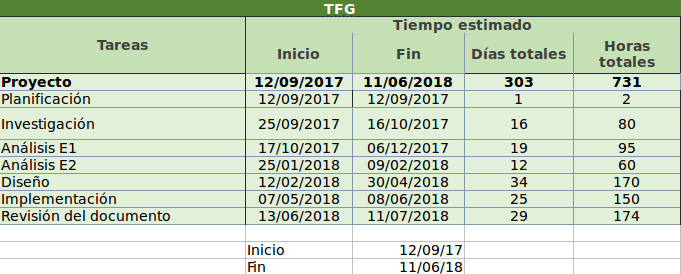
\includegraphics[scale=0.6]{pictures/planificacion.png}
	\caption{Tabla de planificacion del proyecto}{Tabla de planificacion del proyecto.}
    		\label{fig:Tabla de planificacion del proyecto}
\end{center}
\end{figure}
Si echamos un vistazo al diagrama de Gantt obtenemos de estos datos, se puede observar claramente que el esfuerzo ha estado bastante espaciado en el tiempo. Estando centrado especialmente en el inicio y final del proyecto. También el tiempo, al poco de comenzar el proyecto, el tiempo el que el proyecto estuvo parado por dedicarle tiempo a terminar las asignaturas pendientes durante el primer cuatrimestre.
\begin{landscape}
\begin{figure}[htb]
\begin{center}
	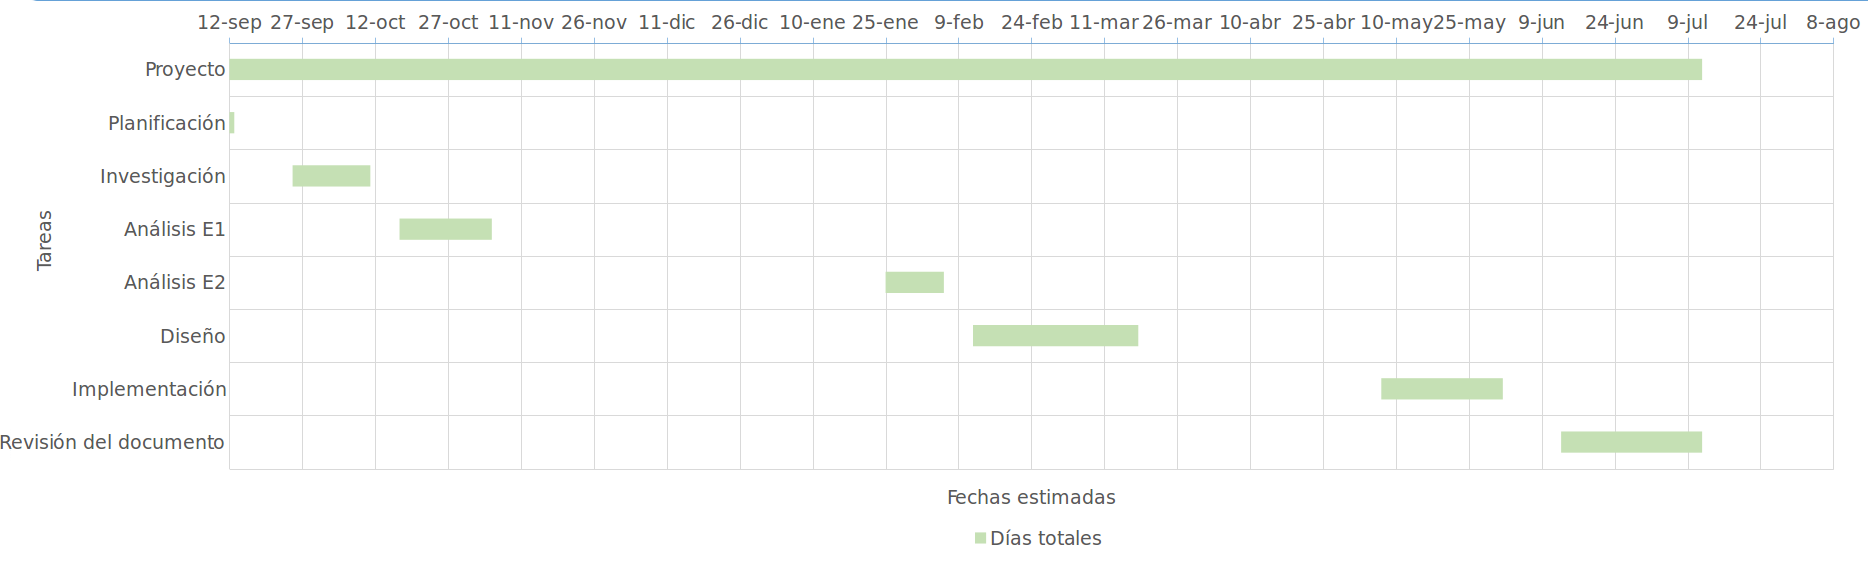
\includegraphics[scale=0.47	]{pictures/planificacion_grafica.png}
	\caption{Diagrama de Gantt}{Diagrama de Gantt.}
    		\label{fig:Diagrama de Gantt}
\end{center}
\end{figure}
\end{landscape}

\chapter{Estado del Arte}
Está claro que para este proyecto no estamos inventando la rueda, el rastreo del usuario es una técnica que existe prácticamente desde que el uso de internet se hizo mayoritario, por ello vamos a ver como ha evolucionado este rastreo y captura a lo largo de los años. 
\newline \newline 
Comenzaremos viendo las técnicas de análisis web, implantadas desde hace décadas, como primera forma de conocer a los usuarios a través de sus visitas a páginas y aplicaciones web. 
\newline \newline
Siguiendo el mismo camino que ha marcado el desarrollo de la tecnología, veremos como estas técnicas se han adaptado, persiguiendo el mismo objetivo, a los Smartphones, centrándonos además en el ecosistema Android. 
\newline \newline 
Por último veremos el caso de los dispositivos IOT que poco a poco comienzan a hacer su aparición en el mercado, nos referimos a asistentes personales como Amazon Echo ó Google Home, de reciente aparición pero con potencial para instalarse en los hogares de muchas familias.
\newpage 
\section{Análisis Web}
Entendemos por análisis web la medición, recolección, análisis y procesado de los datos generados  la  navegación  con la idea de comprender y optimizar el uso de una determinada página. 
\newline \newline
Este análisis no se limita únicamente a la medición del tráfico, si no que puede utilizarse como una herramienta de negocio mediante la cual mejorar el \textit{marketing} y el impacto de una web, además de aportar la información necesaria para realizar campañas publicitarias por zonas geográficas, variables demográficas, etc. Se trata entonces de establecer un perfil de usuario y comprender las tareas que realiza dentro de un sitio a través del \textit{tracking}. Este \textit{trackeo} puede hacerse de distintas maneras, muchas veces implementando todas ellas para obtener información más completa.
\subsection{Geolocalización}
A través de la dirección IP es posible conocer la localización del usuario en distintas granularidades, que van desde el país hasta la ciudad. 
\newline \newline
Esto es posible gracias a la propia naturaleza del protocolo TCP/IP \cite{manolito}, donde a cada dispositivo de acceso a Internet se le asigna una dirección única que identifica la conexión. Además, como se ha estudiado durante la carrera, esta dirección IP que identifica al usuario va adjunta en los datagramas de las peticiones generadas durante la navegación, quedando registrada como IPorigen de la conexión. 
\newline \newline
De esta forma, ya sabemos que nuestra dirección IP viaja continuamente en cada comunicación que establecemos en internet, pero ¿quién controla y registra la vinculación de una dirección con un espacio físico? Hay diversos organismos, que a través de la organización \textit{Regional Internet Registry} (RIR) \cite{RIR}, se dedica a supervisar la asignación y registro de recursos de números de internet en cada región del mundo. Tenemos así 5 RIR en funcionamiento, una por cada continente. 
\newline \newline
Gracias a estas organizaciones es posible saber la situación geográfica de cada dirección, conociendo además detalles de la conexión \cite{ripe} como los servidores DNS utilizados, los puntos de acceso por los que ha pasado la conexión para realizar el \textit{routing}, etc. A continuación se adjunta una captura de la información obtenida al consultar la IP en la propia plataforma del RIPE. 
\begin{figure}[H]
	\begin{center}
   		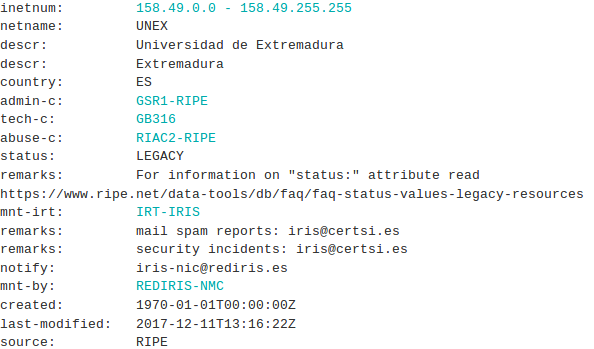
\includegraphics[scale=0.5]{pictures/data/ripedata.png}
	    	\caption{Datos obtenidos mediante RIPE}
   		\label{fig:Datos obtenidos mediante RIPE}
	\end{center}
\end{figure}
Se puede 
\subsection{Análisis de los gestos del ratón}
Este tipo de captura y análisis está centrado en el movimiento que hace el usuario a lo largo de la pantallla y los clicks realizados con el ratón sobre los diferentes enlaces que componen la interfaz. 
\newline \newline
Normalmente, la información que se obtiene por este método es útil tanto para desarrolladores, diseñadores y redactores de una página a la hora de evaluar el rendimiento, diseño y conocer los contenidos más relevantes, respectivamente. Esta técnica es tremendamente útil puesto que permite conocer cómo se \textit{mueven} los usuarios dentro de un sitio, que secciones dentro de una página visitan más, incluso generar mapas de calor con las zonas por las que más se mueven los usuarios y detectar así puntos calientes a los que prestar más atención, así como fugas de interés, encontrando puntos ciegos, para proceder a un análisis de las causas y mejorar así el rendimiento de un portal. 
\newline \newline
Desde un punto de vista técnico, esta recolección de datos puede ocurrir en tiempo real o bien los datos serán almacenados para manipularlos después. A día de hoy muchas \textit{suites} analíticas implementan esta funcionalidad a través de código Javascript insertado en las páginas con métodos que capturan y rastrean la interacción del ratón dentro de la página. 
\newline \newline
Este método a ido evolucionando con el tiempo hacia nuevas aproximaciones, como la predicción del click, donde mediante un programa que siga el movimiento del ojo del usuario y midiendo la dilatación de su pupila podemos predecir donde se realizará la pulsación y adaptar así la respuesta del servicio a la nueva situación prevista \cite{guachos}. 
\subsection{Cookies}
Las cookies, aunque estén tan de moda últimamente con la salida del \textit{nuevo} RGPD \cite{rgpd} (Reglamento General de Protección de Datos) sustituyendo a la nacional LOPD (Ley Oficial de Protección de Datos), surgieron en los albores de internet, siendo el primer método de \textit{rastreo} utilizado. 
\newline \newline 
Las cookies surgieron por la necesidad de mantener información sobre la sesión del usuario después de un login, mantener los elementos de un carrito de la compra o sencillamente para guardar información sobre preferencias del sitio (idioma, tema...). 
\newline \newline 
Estas cookies consisten en un par clave-valor que, generado por el servidor, es enviado al cliente para que este lo almacene en local. Más tarde esta información es consultada para adaptar el contenido en base a esa información.  
\newline \newline
En teoría, una cookie solo puede ser consultada por su origen, es decir, por el servidor que la generó, pero con el tiempo y la aparición de servidores compartidos (servidores de publicidad, por ejemplo) es posible generar una cookie que podrá ser consultada por todas las páginas que empleen ese servidor, estas son las llamadas \textit{third party cookies}, que guardan o usan información del usuario sin que este tenga que navegar directamente en su dominio, dado que está incrustada en la web anfitrión. 
\newline \newline 
Entre la información que es posible capturar con una cookie se incluye el sistema operativo, la dirección IP, el navegador, la ubicación, uso horario, idioma y lo más importante, los sitios por los que se navega. Por ejemplo, si se busca en una tienda online (pongamos Amazon como ejemplo), esa información sobre la búsqueda se queda almacenada en la cookie. Si otra web emplea publicidad de esa tienda, sabrá los términos de la búsqueda y podrá mostrar publicidad relacionada. 
\newline \newline 
Normalmente, la técnica para el rastreo con cookies pasa por la creación de un identificador único de usuario para asociarlo a la misma. Este ID nos mantendrá identificados durante nuestra navegación y será empleado por las páginas que usen los servicios del proveedor de esa cookie. De esta manera, si cada página emplea cookies propias o de terceros, seremos conscientes de que estamos continuamente generando información y que además esta información no pasa desapercibida, si no que es registrada, enviada, usada y compartida entre compañías. 
\section{Google y la plataforma Android}
Hasta ahora hemos visto los métodos de captura de información a través de la web, pero en los últimos 10 años el mercado ha cambiado mucho con la aparición del smartphone. Las cifras son apabullantes, en 2008 nace Android y en el tramo de 10 años la implantación del smartphone en la sociedad está fuera de cualquier duda. 
\begin{figure}[H]
	\begin{center}
   		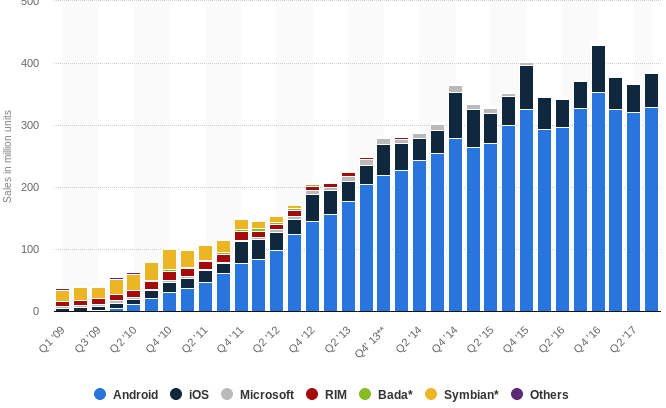
\includegraphics[scale=0.5]{pictures/data/smartphone_sells.png}
	    	\caption{Venta global de smarthpones según el sistema operativo}
   		\label{fig:Venta de Smartphones}
	\end{center}
\end{figure}
Es por tanto una línea muy a tener en cuenta, estamos hablando que llevamos un dispositivo inteligente con nosotros todo el día, se ha convertido en una extensión más de nuestro cuerpo. Un pedazo de tecnología que nos permite estar conectados 24 horas al día, sin interrupción. 
\newline \newline
Pensar que aún teniendo eso en el bolsillo aún somos anónimos es pecar de insensatos, cuanta más conexión mayor control. Las grandes compañías, en su afán por conocer a sus usuarios, no desaprovechan este hecho, aunque a nosotros muchas veces se nos pase por alto. Llevamos en nuestro bolsillo un aparato que no deja de ser un ordenador miniaturizado, que nos permite comunicarnos con nuestros contactos, acceder a Internet y usar servicios que nos hacen la vida más fácil. Pero no se paga nada, a parte del coste del propio dispositivo físico. 
\newline \newline
Recordemos entonces las palabras citadas al inicio del trabajo, cuando no pagas por un producto es porque el producto eres tú. Consumimos tecnología mientras que la tecnología nos consume a nosotros, usamos teléfonos cuyo código fuente sólo es accesible para los creadores del mismo, no sabemos que llevamos encima, en el bolsillo, un aparato que expande nuestras capacidades de comunicación como nunca antes ha sucedido en la historia de la humanidad. 
\newline \newline
Personalmente, creo que esto debería y que realmente está empezando a cambiar, si el teléfono es una parte más de nuestro cuerpo (algo incuestionable), deberíamos aplicar el mismo celo que al resto de cuestiones de nuestra vida. Del mismo modo que no consumimos determinados productos (por ejemplo, gente que evita los transgénicos, carnes rojas, etc) deberíamos comenzar a plantearnos el origen de ese \textit{cacharro} que llevamos todo el día en nuestro bolsillo, con el que compartimos nuestra intimidad y usamos para hablar con amistades y seres queridos. 
\newline \newline
En el caso que nos atañe, Android, viene de la mano de Google, empresa que vive (entre otras cosas) del \textit{segmentation-targeting}. Quieren nuestros datos y nosotros se los damos sin pestañear. Incluso siendo conscientes de que nuestras costumbres están siendo analizadas, perfiladas y almacenadas dentro de un modelo, no dejamos de consumir sus servicios. 
\newline \newline
Esa esclavitud tácita está con nosotros desde que abrazamos la tecnología, cada vez más conectados, cada vez más esclavos. Por ello, es bueno mirar con ojos críticos a las compañías a las que entregamos nuestras vidas (la vida digital y real están tan mezcladas que hacer distinciones es absurdo) y pararnos a pensar que sucede realmente con nosotros, los consumidores. ¿Realmente no estamos pagando nada por los servicios que se nos ofrecen? ¿Deberían pagarnos ellos a nosotros por invadir nuestra privacidad? ¿Asumimos el coste que conllevan las facilidades que este modelo de consumo tecnológico nos ha impuesto?. 
\newline \newline
Veamos cuánto de verdad hay en estas palabras y si realmente existen casos documentados de que esto esté sucediendo así. 
\subsection{Los servicios de Google y la localización}
Durante el 2017 salió a la luz la noticia de que Google registraba y almacenaba la localización de los teléfonos Android incluso cuando este servicio estaba desactivado \cite{googleLocalizacion}. Esto fue confirmado poco después por Google, quien afirmó que abandonaron esa práctica al poco de darse a conocer estos hechos. 
\newline \newline 
Es lógico pensar que cuando estamos usando algún servicio de google que incluya localización esta se mande a sus servidores, son sus reglas y si quieres usar el servicio es un coste asumido. De hecho, Google no oculta esta práctica, pudiendo consultar tu histórico de localizaciones en su propio portal \cite{googleLocationHistory}. A continuación se adjunta la imagen del histórico de localizaciones del autor en la ciudad de Cáceres. 
% IMAGEN 
\begin{figure}[H]
\begin{center}
	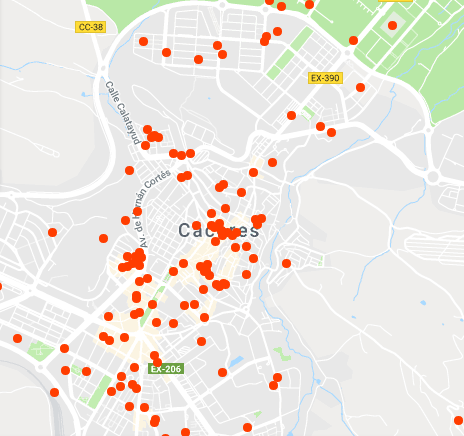
\includegraphics[scale=0.5]{pictures/data/google_location_history.png}
	\caption{Historial de localizaciones en Cáceres}
	\label{fig:Historico de localizaciones}
\end{center}
\end{figure}
Por lo tanto, esta práctica de Google no es ningún secreto, siendo además una \textit{feature} de su sistema y sus servicio de mapas, ofreciendo rutas alternativas al itinerario habitual en función del tráfico, guardar la posición del aparcamiento, etc. 
\newline \newline 
El problema viene cuando se pierde el control de esta información. La  noticia citada al principio de esta sección pone en relieve la problemática, puesto que Google envía información de tu localización a sus servidores incluso cuando este servicio está desactivado en el teléfono y la SIM quitada. 
\newline \newline 
Pero, ¿cómo sabe Google donde estás si tienes este servicio desactivado? Aprovecha las antenas de telefonía. En primer lugar se identifica al usuario por su CellID (identificador único de cada teléfono) y cada vez que el terminal se conecta a una torre se manda la información de esa conexión junto con el cellID a sus servidores. Esa información de la conexión incluye el identificador de la torre, que permite saber su localización exacta. 
\newline \newline 
En un primer momento pudiera parecer que esta práctica no es demasiado intrusiva, solamente se manda información sobre la torre más cercana a la que se ha conectado el teléfono, pero cuando esta práctica se extiende a lo largo del tiempo (durante 24 horas por ejemplo), se puede llegar a triangular la posición exacta del teléfono gracias a la información de las torres a las que se ha ido conectando. 
\newline \newline 
Google reconoció los hechos y aportó más información al respecto, afirmando que además de la información de las torres de telefonía empleaban otros datos, como la cercanía con redes Wifi u otros dispositivos. 
\newline \newline 
Esto hila con otro escándalo que esta vez esta relacionado con el coche que Google emplea para mapear las ciudades para su servicio de Google Maps. Resulta que este coche, además de fotografiar las calles, iba recolectando la información de las redes Wifi abiertas, obteniendo así un mapeo de las redes y su localización exacta \cite{gmaps}. 
\newline \newline
Con estas fuentes de datos es tremendamente sencillo para Google saber que está haciendo el usuario en cada momento, puesto que es posible determinar si estás en un núcleo urbano, en lo alto de una montaña, si vas andando, bicicleta, usas el transporte público, etc. Esta información es tremendamente útil para hacer crecer la base de conocimiento de Google y mejorar el targeting de su servicio de publicidad (AdWords). 
\subsection{Aplicaciones de terceros}
Hemos visto como Google aprovecha su propia plataforma para registrar datos del usuario, veamos ahora como otras compañías se aprovechan de ella para recolectar información de los usuarios a través de las aplicaciones que implementan para este mismo sistema. 
\subsubsection{Aplicación de La Liga}
A principios de Junio de 2018 salió a la luz un nuevo caso de espionaje al usuario. En esta ocasión se trataba de la aplicación oficial de La Liga \cite{noticiaLaLiga}, la cual usaba el micrófono de los usuarios para, en teoría, detectar posibles fraudes. 
\newline \newline 
Para ello la aplicación pedía permisos de micrófono y de localización para, de nuevo supuestamente, activar esta funcionalidad en las franjas horarias de los partidos de fútbol y analizando el audio capturado junto con la localización, detectar posibles fraudes. 
\newline \newline 
El revuelo vino porque los usuarios no eran conscientes de que esto sucediese, lo cual dice muy poco de nosotros como usuarios, se estaban aceptando unas condiciones legales en las figuraba una línea indicando claramente este uso, así como la autorización explícita a la aplicación para usar el micrófono. 
\newline \newline 
Al poco tiempo de que la noticia salía a la luz la empresa realizó un comunicado donde se repetían lo dicho arriba, que ese audio era únicamente para detectar fraudes en el territorio Español y no era usado para otros propósitos. Dada la vaguedad de las declaraciones, hubo usuarios que analizaron la aplicación y estudiaron su comportamiento \cite{laLigaJaker}, lo que nos permite hacer un resumen de como está implementada esta lógica. 
\newline \newline 
En primer lugar, la aplicación comprobaba los permisos de micrófono y localización en cada ejecución, solicitándolos en caso de no estar asignados. Después, mediante un listener, detecta cada cambio de ubicación y va creando un registro que, cada 30 minutos, se manda a un servidor y se borra del teléfono. 
\newline \newline 
El micrófono, en cuanto está disponible, comienza a grabar y mandar los archivos al servidor. Durante cuanto tiempo permanece activa esa grabación es un misterio, así como el comportamiento de la activación del micrófono, puesto que lo lógico sería pensar que la aplicación, en función de la localización y el horario, active el micrófono, pero el análisis del código rebela que esta activación es arbitraria y nada tiene que ver con cuándo suceden los partidos de fútbol 
\newline \newline 
Esto ha demostrado que la escucha a los usuarios por parte de las compañías es una práctica que está a la orden del día, de hecho, cada vez son más las voces que afirman que Facebook a través de su aplicación emplea el micrófono para escuchar conversaciones privadas y aunque Facebook ha negado siempre esta práctica, las sospechas siempre estarán ahí, quedando demostrado además, como acabamos de ver, que ésta práctica existe y lo preocupante realmente es saber que pasa con ese archivo de audio desde el momento en el que sale del teléfono, puesto que se pierde cualquier control sobre estos datos. 
\subsubsection{Aplicación Linterna}
En este caso, vamos a irnos a una aplicación que saltó a la palestra a lo largo de 2013, cuando se descubrió que una aplicación a primera vista inocente dedicada a activar el led de la cámara y proveer así de una linterna, mandaba los datos de ubicación de sus usuarios a sus servidores junto con datos acerca de las redes wifi disponibles para más tarde vender los datos a terceros. 
\newline \newline 
Este caso está ampliamente documentado, llegando a publicar un comunicado de la Comisión Federal del Comercio de EEUU (un homólogo al patrio FACUA) donde se describen y condena esta práctica \cite{CFCEEUU}. 
\newline \newline 
En el documento citado se condena a la compañía por estas acciones, entre las que se incluyen la posibilidad de tomar fotos a través de la cámara del dispositivo sin que el usuario tome partido en ello y el envío de datos de localización a empresas de publicidad. 
\newline \newline 
Este caso nos sirve como muestra, junto con el anterior, de que estas prácticas llevan muchos años en el sector y pone en relieve la falta de control de los datos del usuario, además, nos hace plantearnos que hacen las grandes compañías con sus aplicaciones, en las que entra en juego mayor alcance de usuarios y por tanto mayor rédito económico. 
\section{Dispositivos IOT}
En los últimos años hemos visto como \textit{el internet de las cosas} ha comenzado a implantarse en los hogares, desde bombillas inteligentes que podemos controlar con nuestro teléfono hasta frigoríficos que nos avisan cuando falta algún producto en la nevera. 
\newline \newline 
Esta evolución ha seguido su camino y las compañías no han querido perderse la fiesta, desarrollando cada una sus propias versiones de asistentes personales para, en teoría, facilitarnos la vida dentro de nuestra casa, es el caso del Google Home de Google, Alexa de Amazon o el Apple homePod de Apple. Estos dispositivos comparten todos la característica de  activarse mediante comandos de voz, lo cual implica una escucha pasiva en segundo plano a la espera de reconocer algún comando y activarse. 
\newline \newline 
Esta tecnología, dado su enorme potencial, hizo que muchos usuarios mirasen con lupa a estos dispositivos, dando como resultado lo que veremos a continuación. 
\subsection{Asistentes personales}
En este último año han irrumpido en el mercado los asistentes personales, introducidos por Google, Amazon y Apple. Estos asistentes son precisamente eso, un asistente personal que nos ayuda a gestionar nuestra agenda, consultar Internet e interactuar con el ecosistema de cada compañía. 
\newline
\newline
Todos comparten la misma funcionalidad básica, incorporan un micrófono que permanece siempre activo esperando a recibir el comando de activación. Normalmente este comando es una palabra clave que permite que el dispositivo se active, Ok Google! en el caso del Google Home, Alexa… en del Amazon Echo, etc. Una vez el dispositivo está activo pasa a un estado de escucha activa donde atiende las consultas del usuario a través de la voz. 
\newline
\newline
No hay duda de que se tratan de aparatos tremendamente interesante y que a día de hoy es hacia donde se dirige el mercado, Meter en casa un dispositivo con inteligencia artificial que nos facilite la vida, podamos encender la televisión, reproducir música, hacer anotaciones, llamar a nuestros contactos, etc, gestionado únicamente por voz es un producto realmente atractivo.  
\newline
\newline
Pero como hemos estado viendo hasta ahora, las compañías quieren nuestros datos, meter en nuestros hogares dispositivos inteligentes que se encuentran siempre escuchando en segundo plano, a estas alturas, no parece una decisión muy prudente. 
\newline
\newline
Esto demuestra el afán de las compañías por descubrir más de sus usuarios, uno de los grandes escollos que tienen hasta el momento es que sólo capturan la información cuando el usuario interactúa con sus servicios, pero permanecen a ciegas el resto del tiempo. Si consiguen meter en los hogares estos aparatos, que permiten escuchar conversaciones privadas en cualquier momento, aumentará su capacidad de recolección de datos y por tanto mejorar infinitamente su \textit{targeting}, puesto que no sólo sabrán lo que hace el usuario cuando usa su aplicación, si no que les permitirá saber como se comporta durante su vida privada. 
\newline
\newline
En el caso de Amazon Alexa ha quedado demostrado que el dispositivo realiza escuchas aleatorias \cite{alexaSpy}, de duración indeterminada, que, hasta donde se ha podido averiguar, quedan almacenadas en el dispositivo. No es así en el caso del Google Home, donde todos los fragmentos de audio que se registren son enviados a sus servidores, de hecho lo dejan bien claro en su política de privacidad \cite{GooglePrivacy}
\newline
\newline
Esto demuestra el afán de estas empresas por conocer cada vez más detalles de sus usuarios, hasta el punto de perseguir el objetivo último de que todos los hogares cuenten con un dispositivo inteligente que les permita conocer los hábitos de sus usuarios en su vida privada. 
\newline
\newline
Este afán queda explicado cuando reparamos en el problema que llevamos denotando durante el desarrollo de estas páginas, la información recogida, hasta ahora, es parcial, sólo nos muestra al usuario cuando usa sus productos, el resto del tiempo permanece invisible para ellos. Si finalmente consiguen su objetivo (un dispositivo en cada casa) conseguirán saltar esa brecha y poder obtener un perfil completo del usuario, sabiendo qué dice, hace y cómo se comporta a lo largo de las 24 horas del día, sin interrupción, los 365 días del año. 
\newline
\newline
Justo ese es el objetivo de este trabajo, lo cual nos indica que no vamos del todo mal encaminados. Cada vez es más importante conocer a nuestros usuarios, pero hasta ahora este conocimiento estaba limitado al producto en sí, si conseguimos extraer un perfil de comportamiento completo del mismo tendremos en nuestras manos una información con un enorme potencial, que nos permitirá abrir nuevas líneas de investigación, las cuales, en buenas manos, podrán cambiar para bien la vida de muchas personas. 
\newline
\newline
Lo que se persigue con este proyecto es que esta información no esté exclusivamente en manos de grandes compañías, que sólo quieren ver incrementados sus beneficios, si no que sea accesible para cualquier equipo de desarrollo que tenga buenas intenciones (en nuestro caso, el equipo del SpiLab de la Epcc). 
\newpage
\chapter{Requisitos del proyecto}
En esta capítulo se analiza el problema planteado por el proyecto y se detalla su descomposición como requisitos de un sistema software. No hay que perder de vista que nuestro objetivo final será monitorizar las aplicaciones del usuario y registrar información acerca de cómo éste interactúa con el medio.
\section{Requisitos}
Se propone el desarrollo de una aplicación móvil que, en segundo plano, registre los movimientos del usuario y la interacción que realiza con el teléfono. Este registro de actividad debe cubrir los requisitos listados a continuación para componer un sistema final que satisfaga los objetivos expuestos con anterioridad.
\newline \newline 
Por un lado, queremos registrar aplicaciones del usuario. Esto, dicho así en términos generales, no nos sirve de nada. Por ello, en primer lugar, deberemos decidir en que campos de los distintos usos que, como usuarios, le damos teléfono,  nos vamos a centrar. Una vez establecidos estos campos, elegir de cada uno una serie de aplicaciones que cubran nuestros objetivos. 
\newline \newline 
Por lo tanto, nos vamos a encontrar con cinco grandes grupos de aplicaciones. Por un lado la comunicación, siendo esta la razón de la existencia de la telefonía, no podía quedarse fuera. Nuestro objetivo será entonces capturar que tareas desarrolla el usuario en áreas como la comunicación inmediata, donde el usuario habla con sus contactos (las olvidadas llamadas telefónicas) y en la comunicación \textit{asíncrona}, medios tradicionales de comunicación con los contactos, como pueden ser el envío de correos electrónicos o los vetustos mensajes de texto.  
\newline \newline 
Así pues, incluiremos dentro del \textbf{grupo de comunicación}, la aplicación del \textbf{Teléfono}, \textbf{Mensajes} y, dado el auge que tiene Google como proveedor de servicios gratuitos de correo electrónico, capturaremos la aplicación de \textbf{GMail} como punto de entrada a los correos que envía el usuario. 
\newline \newline 
El otro campo en el que nos queremos centrar es, sin duda, más moderno. Se trata de la mensajería instantánea. Desde la aparición del MSN Messenger (allá en el año 99), se produjo una revolución en la manera que los usuarios nos relacionábamos con nuestras amistades, que, hoy en día, se encuentra plenamente implantada en los teléfonos inteligentes. 
\newline \newline 
De esta forma, incluiremos la aplicación más usada a nivel global para \textit{chatear} con los contactos, \textbf{Whatsapp}, como primera aplicación de este grupo. También incluiremos \textbf{Telegram} dado que en los últimos años han conseguido posicionarse como competidores directos de la primera. 
\newline \newline 
Siguiendo con la idea de encontrar los usos habituales que les damos al teléfono, nos encontramos con lo que aporta valor a los terminales de hoy en día, la navegación por Internet. Esto no debería sorprender a nadie, la verdadera revolución de los teléfonos inteligentes consiste en estar siempre conectados a la World Wide Web, es natural entonces que queramos capturar cómo el usuario interactúa con ella.
\newline \newline 
Definimos entonces, como aplicaciones a escuchar dentro de este grupo de navegación por internet, al navegador \textbf{Chrome}. Esto además se nos presenta como una ventaja, y es que los navegadores de las ROMs que los fabricantes imponen en sus terminales son una implementación de este navegador. Y, en un gesto romántico, capturaremos también la aplicación de \textbf{Firefox} como forma alternativa de navegar la web. 
\newline \newline 
Tenemos hasta ahora las áreas de comunicación, mensajería instantánea y navegación web, cubiertas. Si nos planteamos ahora cual es el otro campo donde los móviles han triunfado entre la juventud lo tenemos claro, las redes sociales. Así, escogemos las aplicaciones de \textbf{Facebook} y \textbf{Twitter} como objetivos a escuchar dentro de este área, dada la popularidad de ambas. 
\newline \newline 
Por último, y para completar el abanico de tareas que desarrolla el smartphone, deberemos dirigir la mirada hacia el propio dispositivo. Llamemos a este grupo \textit{sistema}. Por un lado, el terminal es fuente de información para el usuario, esto es así gracias a las notificaciones push que integran la mayor parte de las aplicaciones. Será entonces de gran interés para nosotros, siempre buscando el objetivo de obtener un perfil lo más completo del usuario, el contenido de las notificaciones que entran en su dispositivo. Además, será interesante conocer también los valores de los múltiples sensores que integran los teléfonos modernos, incluyendo, por supuesto, el omnipresente \textbf{GPS}, que nos aportará la información de localización del usuario. 
\newline \newline 
De esta forma, quedan definidos 4 grandes grupos en los que nos centraremos a lo largo del trabajo. Recordemos, comunicación, mensajería instantánea, navegación web, redes sociales y sistema. Todo ello sin olvidar el objetivo fundamental de registrar qué aplicaciones abre el usuario y cuánto tiempo pasa en ellas, independiente de su pertenencia a estos grupos.
\newline \newline 
Además, dada la naturaleza del proyecto, deberemos incentivar al usuario de alguna manera para que se instale la aplicación, así, deberemos incluir toda esta captura en una aplicación que aporte datos del uso que el usuario da al teléfono, aunque sin descubrir toda la información que vamos a capturar. Los datos sobre los tiempos de uso, aplicaciones más utilizadas, tareas frecuentes en esas aplicaciones, se nos antojan interesantes para mostrarlos dentro de la aplicación. 
\newline \newline 
Teniendo estas ideas claras, veamos cual es la especificación de requisitos.  
\subsection{Requisitos funcionales}
El sistema deberá:
\begin{itemize}
  \item Registrar cada aplicación que lanza el usuario detectando y almacenando el nombre del paquete asociado a ella. 
  \item Aportar un contexto temporal de cuando las aplicaciones son ejecutadas, esto es, el \textit{timestamp} del momento de su ejecución. 
  \item Incluyendo lo anterior, registrar el uso dado a aplicaciones relacionadas con, comunicación, mensajería instantánea, búsqueda web,redes sociales y por último, la información generada por el propio sistema. 
  \item Dentro de comunicación se incluye la aplicación de Gmail, Mensajes (sms) y el Teléfono. 
  \item Dentro mensajería instantánea prestaremos atención a Telegram, Whatsapp Messenger.
  \item Como aplicaciones relacionadas con la búsqueda en la web estarán la Chrome Browser y Google Search. 
  \item En las aplicaciones de redes sociales; Twitter y Facebook.
  \item Dentro del sistema, deberemos escuchar tanto las notificaciones recibidas como los sensores, incluyendo el GPS, acelerómetro, presión, giroscopio y temperatura.
    \item La información capturada deberá ser persistida en una base de datos local dentro del propio dispositivo. 
  \item Incluir, dentro de la propia aplicación, información acerca del uso que el usuario hace del teléfono, incluyendo datos sobre, aplicaciones más frecuentes, tiempo pasado en cada una de ellas y, en función del campo, tareas más comunes desarrolladas en cada una.
  \item Incluido dentro del propio servicio de captura, se deberá realizar un volcado del contenido capturado almacenado en la base de datos local para, de forma periódica, mandarlo a un servidor en la nube. 
  \item Este servidor en la nube deberá tener credenciales de acceso y contará con los endpoints necesarios para realizar peticiones de tipo POST que nos permitan almacenar la información. 
  \item Del mismo modo, el servidor deberá incluir endpoints de tipo GET que nos permitan acceder a los datos ahí almacenados. 
\subsubsection{Requisitos de las aplicaciones de comunicación}
  \item En  \textbf{Gmail} capturar, la dirección de correo del emisor. 
  \item La dirección de correo del receptor(es). 
  \item El asunto del correo electrónico. 
  \item El contenido, cuerpo de dicho correo. 
  \item La marca horaria del momento del envío. 
  \item En \textbf{Mensajes} se deberá capturar, el destinatario. 
  \item El cuerpo del mensaje. 
  \item La marca horaria del momento del envío. 
  \item En \textbf{Teléfono} se deberá capturar, el destinatario de la llamada. 
  \item Tiempo total invertido en ella. 
\subsubsection{Requisitos de las aplicaciones de mensajería instantánea}
  \item En \textbf{Telegram} capturar, el nombre del contacto o grupo interlocutor. 
  \item Los mensajes enviados en la conversación por parte del usuario. 
  \item En \textbf{Whatsapp} capturar, el nombre del contacto o grupo interlocutor. 
  \item Los mensajes enviados en la conversación por parte del usuario. 
\subsubsection{Requisitos de las aplicaciones de búsqueda en la web}
  \item En \textbf{Chrome} capturar las páginas visitadas. 
  \item La marca horaria del momento de la visita. 
  \item En \textbf{Firefox} capturar las páginas visitadas. 
  \item La marca horaria del momento de la visita. 
  \item En \textbf{Búsqueda de Google} el objeto de búsqueda. 
  \item La marca horaria del momento de la visita. 
\subsubsection{Requisitos de las aplicaciones de redes sociales}
  \item En \textbf{Twitter} capturar, el nombre de los perfiles visitados. 
  \item Los tuits publicados y la marca horaria de la publicación. 
  \item El contenido de los mensajes directos y la marca horaria del envío. 
  \item En \textbf{Facebook} capturar, el nombre de los perfiles visitados. 
  \item Los comentarios hechos en dichos perfiles y la marca horaria de la publicación . 
  \item Los estados compartidos dentro de la red social y la marca horaria de la publicación . 
  \item Las subidas de fotos y su título junto a la marca horaria de la subida. 
\end{itemize}
\subsubsection{Requisitos de la información generada por el propio teléfono}
\begin{itemize}
  \item Deberán registrarse las notificaciones recibidas por el usuario, incluyendo el contenido de la notificación y la marca horaria del momento en el que se recibe.
  \item Del sensor relacionado con la ubicación \textbf{GPS} deberemos registrar cada cambio de coordenadas que registre el teléfono, junto a la marca horaria del instante de la captura. 
  \item Mediante el \textbf{acelerómetro} registraremos los cambios en la aceleración del teléfono, junto a la marca horaria del instante de la captura. 
  \item Con el sensor de \textbf{presión} registraremos los cambios de altitud del teléfono, junto a la marca horaria del instante de la captura.
  \item Con el \textbf{giroscopio} para detectar y registrar  los movimientos que realiza el teléfono, junto a la marca horaria del instante de la captura.
  \item El sensor de \textbf{temperatura} nos permitirá registrar, como no, la temperatura ambiente del dispositivo, junto a la marca horaria del instante de la captura.
\end{itemize}
\subsection{Requisitos no funcionales}
\begin{itemize}
	\item Versión. El sistema deberá soportar una versión limpia de Android 8.0. 
	\item Eficiencia. Dado que el sistema debe registrar en tiempo real toda la información generada por el usuario, deberá ser capaz de capturarla en tiempo real, al mismo tiempo que se analiza y almacena. 
	\item Privacidad. El usuario deberá autorizar explícitamente al software desarrollado permisos de accesibilidad, de modo que sea consciente de que existe una aplicación monitorizando parte de su actividad.
	\item Robustez. Debido a que el sistema debe estar constantemente capturando, el software debe ser tolerante a fallos y mantener el servicio siempre disponible.  
	\item Seguridad. La base de datos local deberá estar protegida ante el acceso indebido a los datos. 
\end{itemize}
\subsection{Conclusiones de la definición de requisitos}
Los requisitos listados en este capítulo tienen como objetivo definir la implementación de un sistema que permita, en última instancia, obtener un perfil completo del usuario. 
\newline \newline 
Por un lado, los requisitos funcionales nos guiarán en la captura de información del usuario. Como se ha visto, tenemos 5 grandes grupos, que nos permiten conocer todas las facetas de la vida de este, ó, al menos, todas las que pasen por usar el terminal. 
\newline \newline
Gracias al apartado de comunicación , escuchando aplicaciones como Gmail, el envío de SMS y las llamadas telefónicas. Con la mensajería instantánea cubrimos las tres grandes aplicaciones en este campo, Whatsapp y Telegram. En la navegación web, otra de las grandes tareas que hacemos con nuestros teléfonos, escucharemos Chrome, Firefox y la barra de Búsqueda Rápida de Google. 
\newline \newline 
También podremos saber como interactúa el usuario con sus contactos a través de las redes sociales, puesto que almacenaremos datos provenientes de Facebook y Twitter. Y por último, para conocer cómo interactúa el usuario con el medio, recogeremos las notificaciones que entran en el dispositivo, así como los datos de los sensores físicos que incorporan la mayoría de terminales. 
\newline \newline 
Todos estos requisitos, junto con los no funcionales, cuyo objetivo es aportarle robustez al proyecto, nos permitirán desarrollar un sistema completo que abarque los usos mayoritarios del teléfono, obteniendo así un perfil completo de cómo un usuario interactúa y se relaciona con su terminal y entorno. 
\break
\chapter{Análisis}
Para centrar el problema y enfocar los requisitos a un proceso que nos lleve a obtener un proyecto de ingeniería, haremos uso de distintos diagramas que nos ayudaran a resolver el problema y plantear una solución. Así en el capítulo nos encontramos con los diagramas de casos de uso, indicando las tareas que debe resolver el sistema, y un diagrama de arquitectura a alto nivel que plantea una solución inicial. 
\section{Diagramas de Casos de Uso}
Los casos de uso del sistema están planteados de modo que el usuario, al interactuar con el teléfono, dispara siempre la acción, aunque en muchos casos la acción del usuario será pasiva, es decir, no tendrá que realizar ninguna acción en concreto para disparar, por ejemplo, la captura de los sensores, pero será su propia actividad la que nos permita realizar dicha captura. 
\newline
\newline
Por lo demás, hemos agrupado las aplicaciones en 5 categorías, comunicación, mensajería, navegación web, redes sociales y sistema. Dado que la mayoría de estas aplicaciones comparten la información a capturar, los veremos agrupados por comodidad para el lector. 
\subsection{Casos de uso generales}
Estos casos de uso describen como se hace la captura de las aplicaciones. Por un lado, tenemos el registro del nombre de la app a través del nombre del paquete, y el timestamp del marco de ejecución para todas ellas. Vemos además como la captura de información extiende del lanzamiento de una aplicación, esto es así porque esta captura no se hará siempre, si no que dependerá de si la aplicación lanzada es objeto de captura. 
%%% ------ 
\begin{figure}[H]
	\begin{center}
		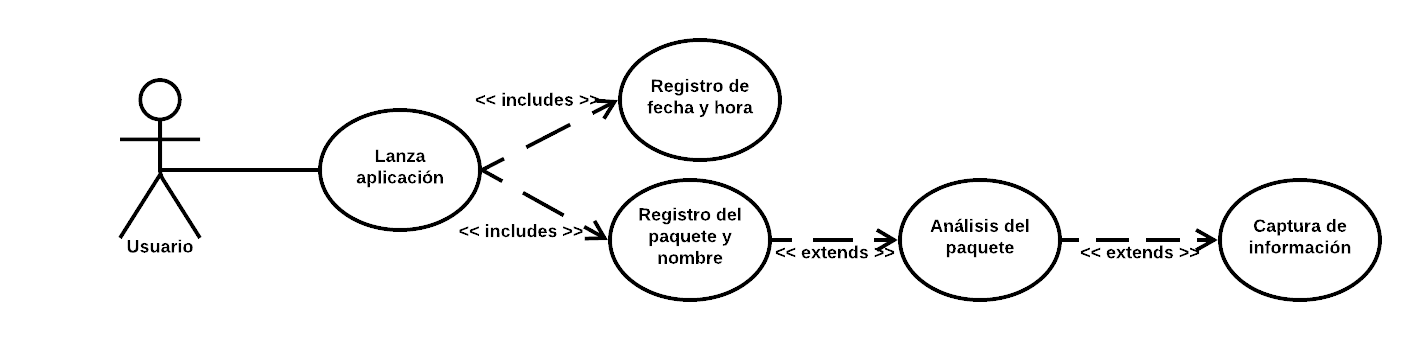
\includegraphics[scale=0.7]{pictures/usecases/usecases01.png} % include ./img/imagen.[pdf|png|jgp] si es pdflatex o ./img/imagen.eps si es latex
	\end{center}
	\caption[Casos de uso de cualquier aplicación.]{Casos de uso de cualquier aplicación.}
\end{figure}
%%% ------
\subsection{Casos de uso de aplicaciones de comunicación}
Si nos centramos en el apartado de aplicaciones de comunicación (GMail, SMS y Teléfono), para Gmail, deberemos registrar el destinatario (o destinatarios, en caso de incluir varias direcciones) del correo, así como su asunto, el cuerpo del mensaje y la marca horaria del momento en el que el correo fué enviado. 
\newline \newline 
Para los SMS, se incluyen las tareas de registrar el interlocutor y el cuerpo del mensaje. En el caso de la captura del teléfono, incluirá el registro del destinatario de la llamada, así como la duración total de la misma.  
%%% ------ 
\begin{figure}[H]
	\begin{center}
		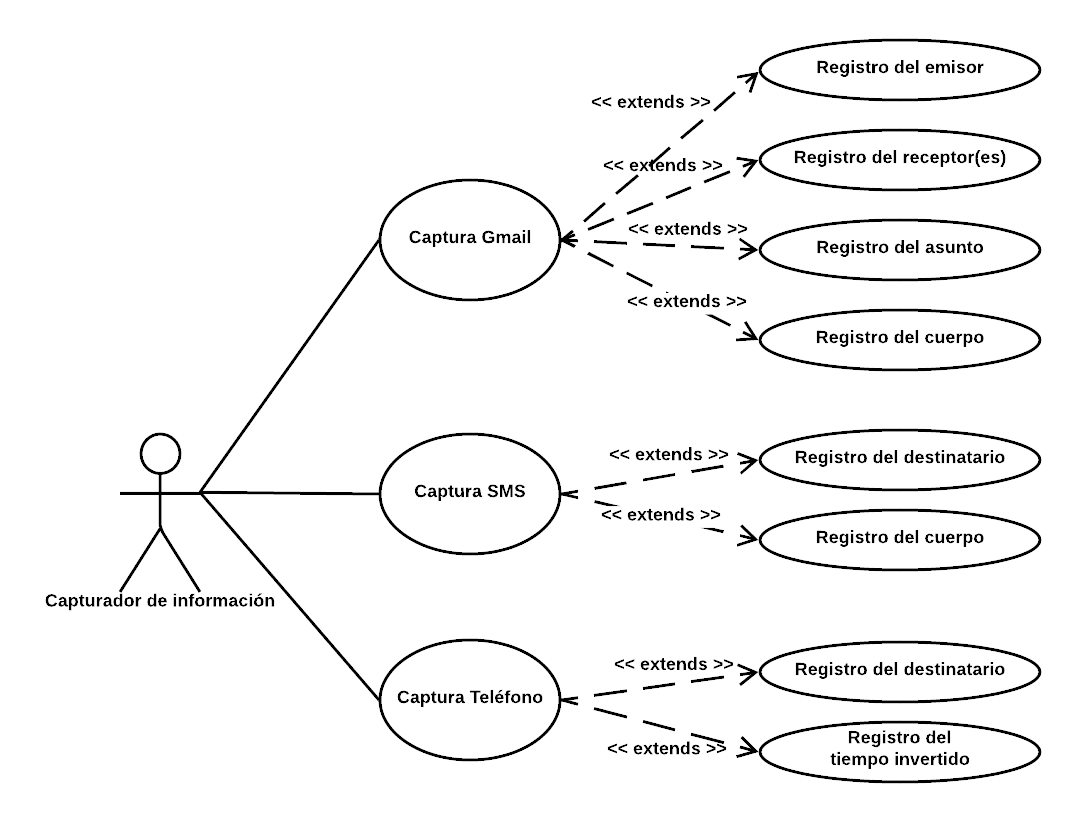
\includegraphics[scale=0.70]{pictures/usecases/usecases02.png} % include ./img/imagen.[pdf|png|jgp] si es pdflatex o ./img/imagen.eps si es latex
	\end{center}
	\caption[Casos de uso de aplicaciones de comunicación.]{Casos de uso de aplicaciones de comunicación.}
\end{figure}
%%% ------
\subsection{Casos de uso de aplicaciones de mensajería instantánea}
En el grupo de mensajería instantánea, donde están incluidos el Whatsapp y Telegram, se incluyen como tareas de la captura, tanto para Whatsapp como para Telegram, el registro del interlocutor y los mensajes vertidos en la conversación. 
%%% ------ 
\begin{figure}[H]
	\begin{center}
		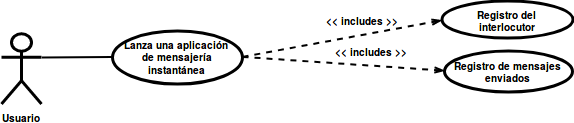
\includegraphics[scale=0.70]{pictures/usecases/usecases03.png} % include ./img/imagen.[pdf|png|jgp] si es pdflatex o ./img/imagen.eps si es latex
	\end{center}
	\caption[Casos de uso de aplicaciones de mensajería instantánea.]{Casos de uso de aplicaciones de mensajería instantánea.}
\end{figure}
%%% ------
\subsection{Casos de uso de aplicaciónes de navegación web}
En las aplicaciones de navegación y consulta de la web, donde se incluyen Chrome, Firefox y Búsqueda rápida de Google, la captura incluye las tareas del registro de la url consultada así como también la marca horaria de la consulta. 
%%% ------ 
\begin{figure}[H]
	\begin{center}
		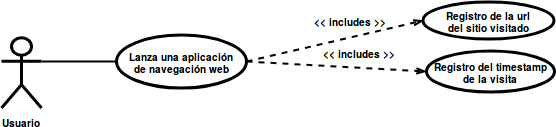
\includegraphics[scale=0.70]{pictures/usecases/usecases04.png} % include ./img/imagen.[pdf|png|jgp] si es pdflatex o ./img/imagen.eps si es latex
	\end{center}
	\caption[Casos de uso de aplicaciones de navegación web.]{Casos de uso de aplicaciones de navegación web.}
\end{figure}
%%% ------
\subsection{Casos de uso de aplicaciones de redes sociales}
Si nos fijamos ahora en las aplicaciones de redes sociales, donde incluimos la aplicación de Twitter y Facebook, vemos que por un lado la captura de Facebook incluye la captura de los perfiles visitados con la aplicación, los comentarios realizados, estados publicados y las fotos subidas con la aplicación. 
\newline \newline 
En el caso de Twitter, la captura incluye el registro de los perfiles visitados, los tuits publicados y los mensajes directos compartidos con la red de contactos de la aplicación. 
%%% ------ 
\begin{figure}[H]
	\begin{center}
		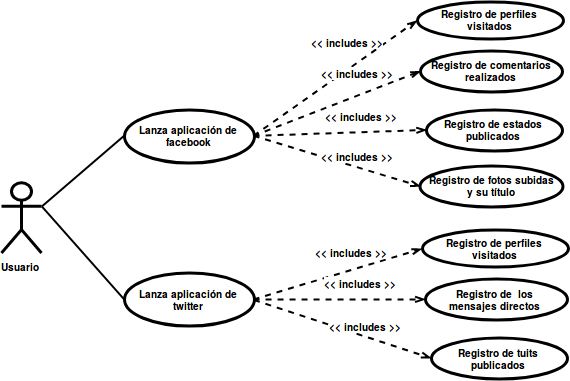
\includegraphics[scale=0.70]{pictures/usecases/usecases05.png} % include ./img/imagen.[pdf|png|jgp] si es pdflatex o ./img/imagen.eps si es latex
	\end{center}
	\caption[Casos de uso de apps de redes sociales.]{Casos de uso de apps de redes sociales.}
\end{figure}
%%% ------
\subsection{Casos de uso para la información generada por el sistema}
Por último, en el apartado de la información del sistema, cada vez que éste genere nueva información, en función de la fuente de origen de la misma, incluimos la captura de las notificaciones que llegan al dispositivo, la posición a través del GPS, y los valores de los sensores de presión, acelerómetro, presión, giroscópio y temperatura.  
%%% ------ 
\begin{figure}[H]
	\begin{center}
		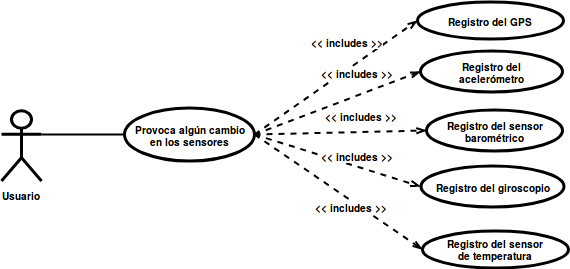
\includegraphics[scale=0.70]{pictures/usecases/usecases06.png} % include ./img/imagen.[pdf|png|jgp] si es pdflatex o ./img/imagen.eps si es latex
	\end{center}
	\caption[Casos de uso de la información generada por el sistema.]{Casos de uso de la información generada por el sistema.}
\end{figure}
%%% ------
\subsection{Casos de uso del volcado de la información}
Del mismo modo, dentro de estos casos de uso generales al sistema, se incluye la tarea de realizar un volcado a un servicio externo, de modo que se asegure la información y se libere espacio en el almacenamiento físico del terminal. 
\begin{figure}[H]
	\begin{center}
		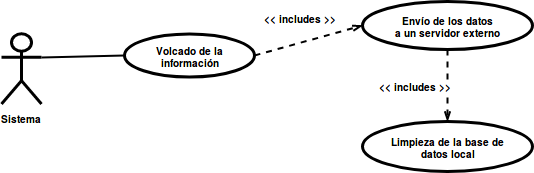
\includegraphics[scale=0.7]{pictures/usecases/usecases07.png} % include ./img/imagen.[pdf|png|jgp] si es pdflatex o ./img/imagen.eps si es latex
	\end{center}
	\caption[Casos de uso de volcado de información.]{Casos de uso de volcado de información.}
\end{figure}
\section{Arquitectura de alto nivel}
Teniendo claro cual es el propósito de nuestro sistema, debemos plantearnos cuáles serán los elementos que, interactuando entre ellos, resuelvan el problema final. 

\begin{figure}[H]
  \begin{center}
     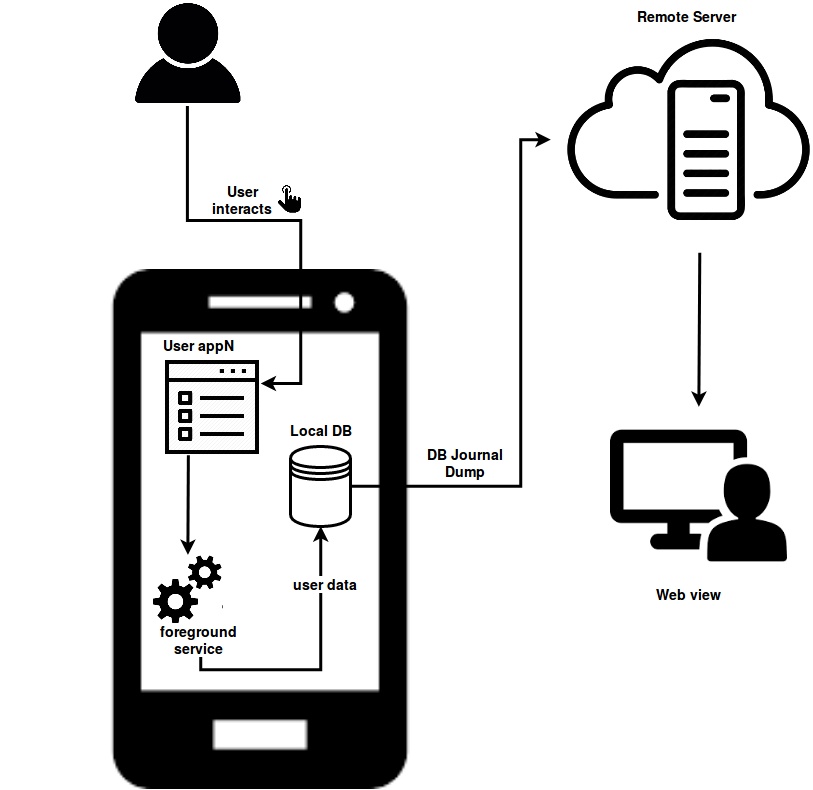
\includegraphics[width=0.8\textwidth]{pictures/architecture/highLevel/altonivel01.png}
  \end{center}
  \caption[Arquitectura de alto nivel]{Arquitectura de alto nivel.}
  \label{fig:Arquitectura de alto nivel}
\end{figure}
%----------- P A N O R A M I C O -------------------------------------------------
Vemos que el sistema se compone gracias a tres componentes fundamentales, por un lado el usuario, fuente de nuestros datos, el propio teléfono, en donde capturaremos la información, y un servidor en la nube que recibirá de forma periódica los datos recogidos por el teléfono y que permitirá además consultarlos. 
\newline \newline 
Estos elementos interactúan entre sí de una forma natural. Por un lado el usuario, el iniciador de toda acción del sistema, interactúa con cualquier aplicación que tenga instalada en su dispositivo. De ella, el \textit{background service} de nuestra aplicación registrará su nombre y el tiempo de ejecución. 
\newline \newline 
Si, además, la aplicación que ha lanzado el usuario se incluyen en alguno de los grupos descritos a lo largo del documento (recordemos, comunicación, mensajería, navegación, redes sociales y sistema), este servicio en segundo plano deberá realizar las labores de cómputo y captura de la información que generada por el usuario al interactuar con ella.
\newline \newline 
Una vez se tenga esta información lista deberá ser almacenada en la base de datos local del teléfono. Será tarea del servicio realizar un volcado periódico de la información a un servidor en la nube. 
\newline \newline 
Este volcado se realiza por motivos de eficiencia, por no saturar el espacio de almacenamiento del teléfono, y además, para poder disponer de los datos en un punto de acceso unificado. El servidor. 
\newline \newline 
Este servidor tiene como único propósito disponer de dos puntos de entrada. El primero, que permita almacenar la información que se envíe desde el teléfono, y segundo, poder consultar la información una vez se encuentre almacenada. 
\newline \newline 
Teniendo en la cabeza cual es el objetivo de cada componente de la arquitectura, y cómo interactúan entre sí, veamos cada elemento de forma separada. 
\subsection{Smartphone}
Vayamos por partes pues y analicemos cada grupo de componentes. Por un lado el \textbf{smarthphone} y el \textbf{usuario}. Dado que el smartphone es la interfaz de acceso del usuario a las funciones del teléfono y sus aplicaciones, será entonces aquí donde centremos nuestro sistema y donde estarán la mayor parte de sus componentes, al menos todos los relacionados con la captura de información. 
\newline
\newline
Este proceso de captura se detalla en el siguiente fragmento de la arquitectura. 
 %%% ------ 
\begin{figure}[hbt]
  \begin{center} \setlength{\unitlength}{0.0105in}
     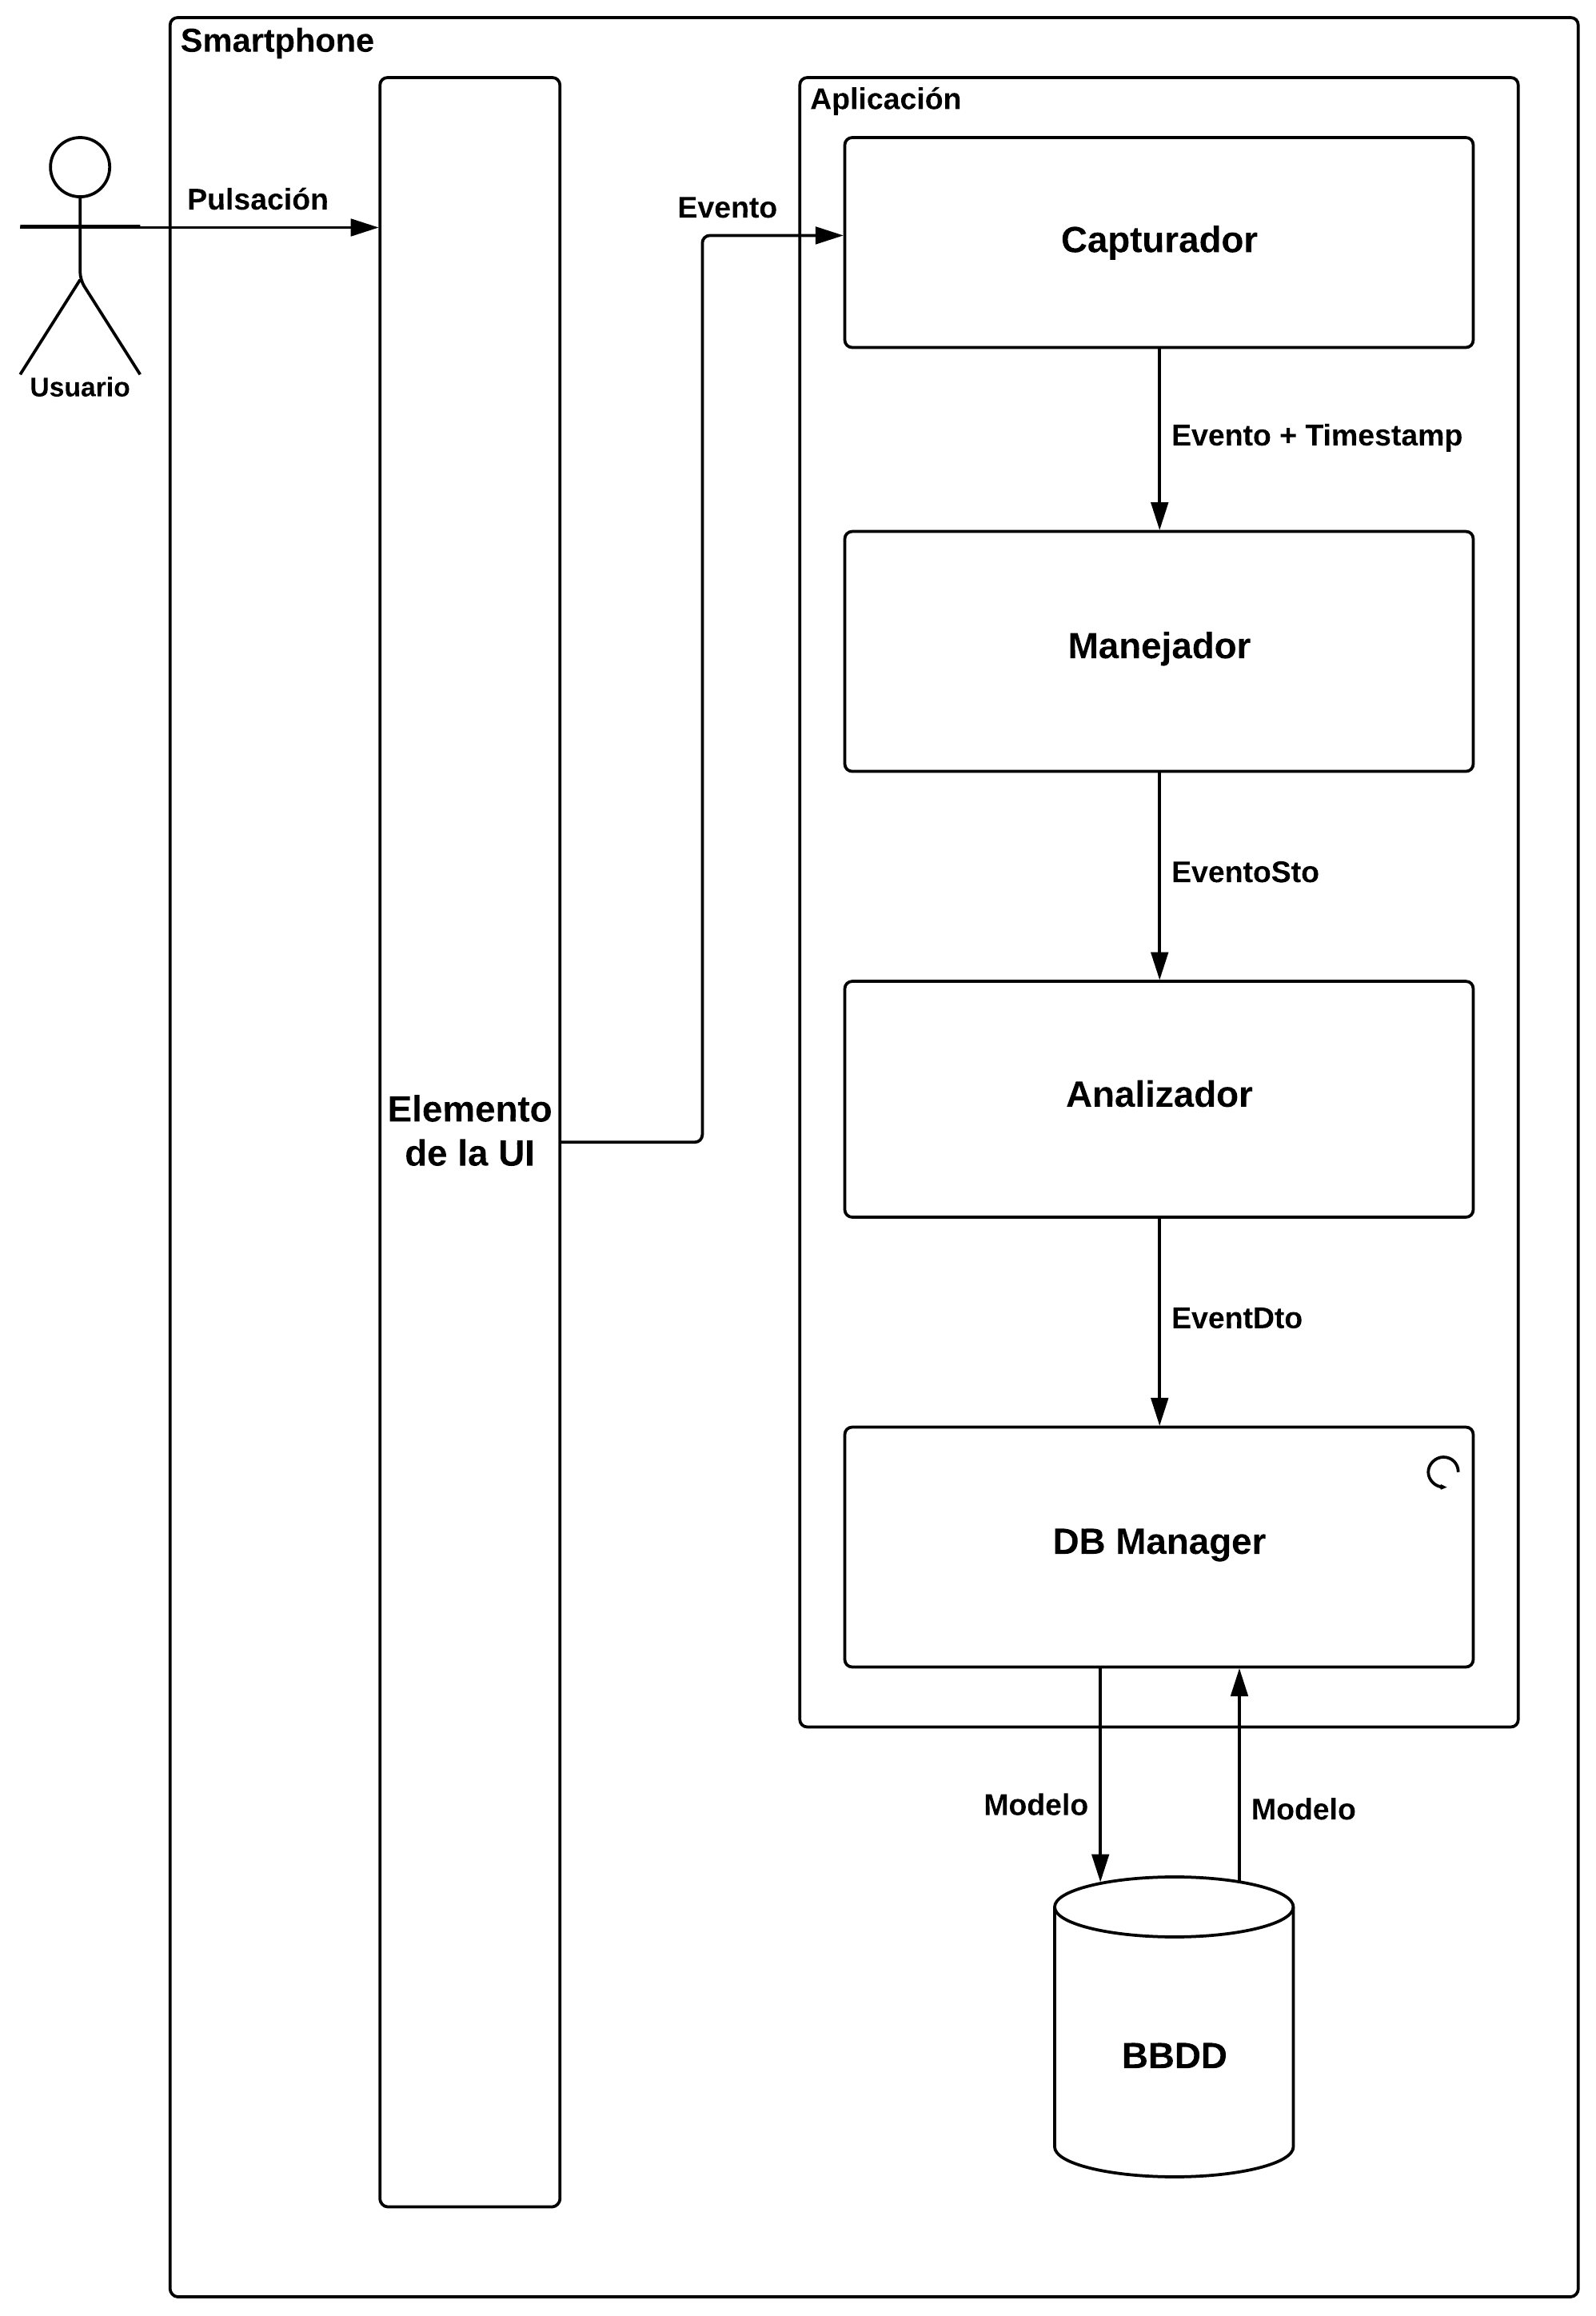
\includegraphics[width=0.6\textwidth]{pictures/architecture/highLevelArch02.png}
  \end{center}
  \caption[Arquitectura de alto nivel. Smartphone]{Arquitectura de alto nivel. Detalle de la parte móvil.}
\end{figure}
%%% ------
Toda la arquitectura parte del usuario, el cual interactúa con su teléfono mediante pulsaciones en la pantalla, que son recogidas por aplicaciones que le devuelven información al usuario mediante esa misma pantalla. Será entonces esta interfaz de usuario lo que nuestro sistema deberá escuchar y capturar. Por lo tanto tendremos una aplicación que recibirá las pulsaciones en los elementos de la interfaz del usuario (UI) bajo la forma de eventos. 
\newline
\newline
Vamos a desglosarla por cada elemento, viendo antes de cada componente la unidad de datos que va a manejar.
\newline
\newline
\subsubsection{Evento}
Estamos ante la información de entrada única y por tanto fundamental del sistema. Se trata de una unidad de datos compleja y sin estructurar. 
\newline
\newline
Los genera el sistema cada vez que ocurre un cambio notable en la pantalla, y su propósito es dar el mayor feedback posible del usuario. 
\newline
\newline
Muchas veces esta información no surge en el instante en el que se produce el evento, que no deja de ser una instantánea de la pantalla en ese momento, si no que se necesita un contexto. Esa es la parte complicada del desarrollo, necesitamos desarrollar sendas máquinas de estado 	que nos ayuden a relacionar los eventos entre ellos y procesarlos de tal modo que se produzca información útil y estructurada. 
\newline
\newline
Es por tanto, una unidad de datos muy cruda y desestructurada a la que hay que extraer el significado en su procesamiento en las capas inferiores. Por tanto este evento será producido por el sistema y la fuente de entrada del nuestro, a través del \textbf{capturador}.
\subsubsection{Capturador}
Se trata de un proceso que está siempre escuchando la aparición de nuevos eventos, con el objetivo de capturarlos y pasárselos al siguiente nivel de la arquitectura, el \textbf{manejador}. Su carga de trabajo realmente será poca, y consistirá en informar al manejador pasándole el evento junto al instante temporal en el que fué generado. 
\newline
\newline
Por lo tanto el capturador recibe eventos y genera eventos junto a su marca temporal para que los consuma el siguiente nivel, manejador. 
\subsubsection{Evento + timestamp}
No consiste en una unidad de datos como tal, puesto que sólo consiste en una fecha y hora y el propio evento asociado a ellos. 
\subsubsection{Manejador}
Recibe un evento y su marca horaria y debe encapsularlo para que el nivel inferior lo analice, es por tanto el nexo de unión entre los datos en bruto y los datos refinados. 
\newline
\newline
Para ello, cuando reciba el evento, en primer lugar lo encapsula junto a su marca horaria en un objeto que hemos llamado Sto. Simple Transfer Object. 
\newline
\newline
Una vez encapsulado, consulta la aplicación fuente del evento, es decir, la aplicación que lo generó, que nos permite establecer nuestro primer filtro y discernir si se trata de gmail, telegram, facebook... etc. 
\newline
\newline
En función de esto, se llamará a una implementación del analizador u otra, puesto que cada aplicación sigue su propio flujo lógico. Por ello se le comunica un Sto con la información fundamental que necesita. 
\subsubsection{Sto}
Es la unidad de datos empleado para comunicar el \textbf{manejador} con el \textbf{analizador}, se trata de una unidad de datos cuyo objetivo es encapsular la información en unidades contenidas y controladas. Será consumido por el analizador a través de la consulta de su evento y su marca horaria, siendo esta última fundamental para aportar el contexto necesario por el analizador. 
\subsubsection{Analizador}
Recibe los citados Stos, objetos sencillos, del manejador, para tratarlos, procesarlos y extraer su significao. 
\newline
\newline
Este procesamiento consisitirá en analizar, en base al modelo correspondiente, el patrón de llegada de los datos y en base a su contenido y el de eventos antecesores y sucesores, aportarle un contexto. Gracias a este modelo construiremos Dtos completos que representarán una unidad de información completa acerca del uso de la app.
\subsubsection{Dto}
Dtos, Data Transfer Objects, será la unidad última de información que genere nuestro sistema, representado así la información completa del usuario, es decir, uno de estos dtos contiene en su interior la interacción completa del usuario con cualquier servicio que le ofrezca el teléfono. 
\newline
\newline
Será por tanto contenido semántico de esta interacción, siendo por ejemplo, un dto una conversación mantenida por whatsapp con un contacto durante el intervalo de tiempo en el que estuvo activa, una búsqueda en el navegador... en resumen cualquier interacción, contextuada, del usuario con cualquiera de las apps que vamos a monitorizar. 
\newline
\newline 
Una vez estos Dtos están listos se les pasa al DB Manager. 
\subsubsection{DB Manager}
Capa encargada de la persistencia de los datos que le pasa el analizador. El manager los convierte en modelos para su almacenamiento en una base de datos local en la memoria del teléfono. 
\newline 
\newline 
En este manager recae una tarea también fundamental para el sistema, puesto que debe realizar un volcado periódico la base de datos a un servidor remoto para su seguridad y almacenamiento para posibles usos. Este funcionamiento de almacenar en local hasta que llegue el momento del volcado se ha tomado teniendo en mente la minimización del número de conexiones con el servicio externo. No podría ser una llamada a la API para persistir la información en la nube cada vez que una unidad de datos esté lista, puesto que la cantidad de información generada al día puede ser ingente. 
\newline \newline
La idea es almacenar en local hasta que pase un tiempo razonable (por ejemplo, 24 horas, tiempo en el que la base de datos se habrá ido llenando poco a poco) para volcar su contenido, liberar espacio y llevar los datos a la nube para persistir y asegurar la propia información. Así, no se satura la memoria interna del teléfono y la información viaja en bloques, minimizando la comunicación con el servicio externo y ahorrando batería, puesto que la conexión se realiza una vez al día. 
\newpage

\subsection{Servidor Remoto}
En este apartado analizaremos la arquitectura del entorno remoto planteado por la arquitectura. Consiste en un servicio en la nube que acepta el volcado que realiza la base de datos del teléfono cada poco tiempo y permite además visualizar los datos allí vertidos. 
 %%% ------ 
\begin{figure}[H]
  \begin{center}
     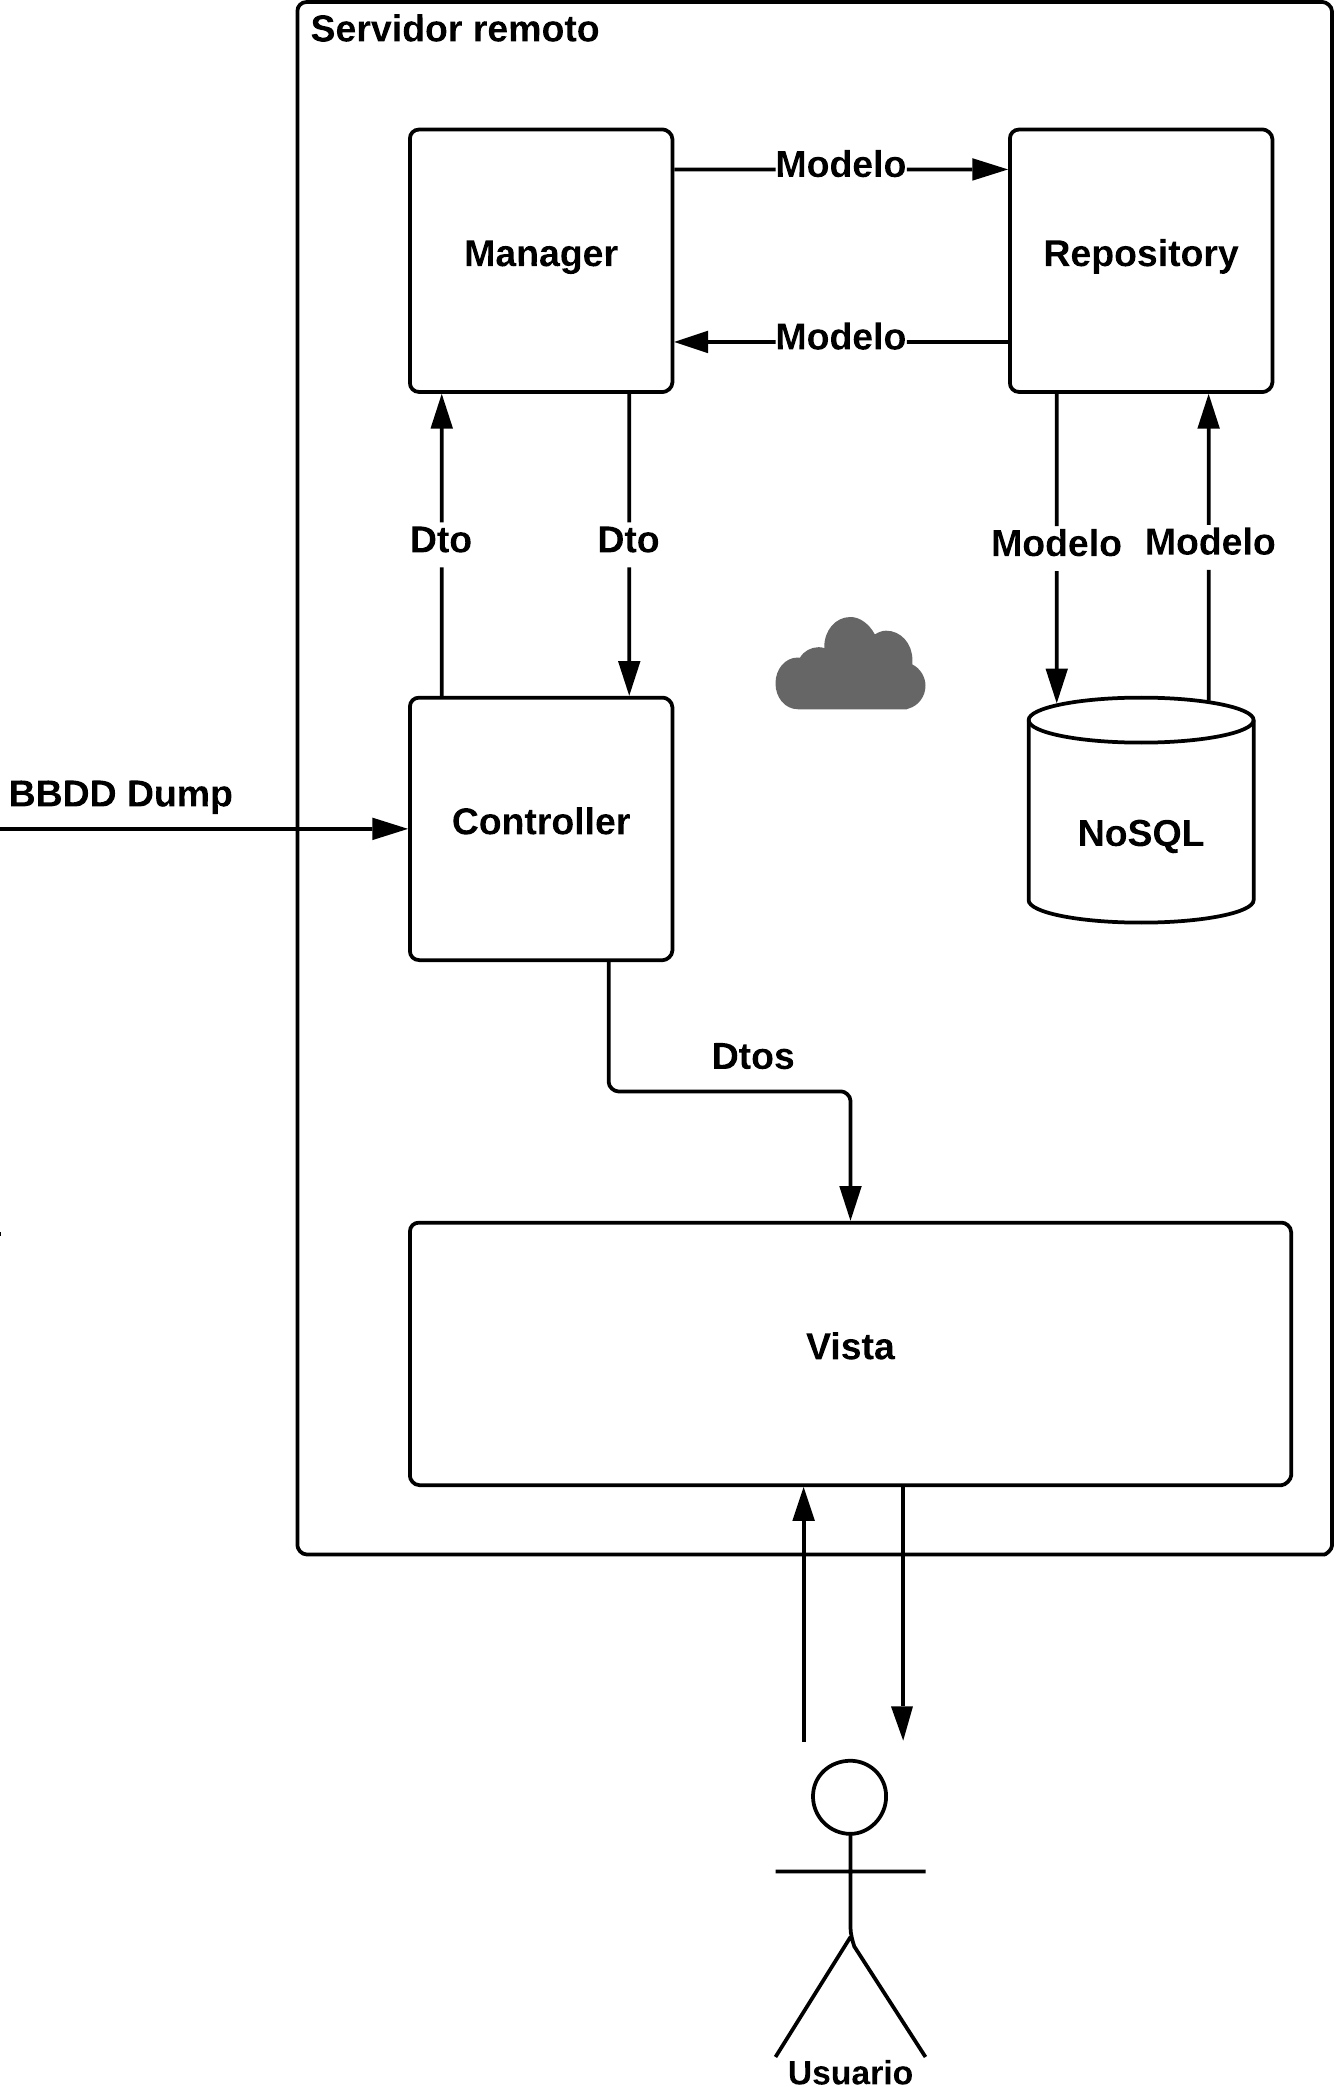
\includegraphics[scale=0.8]{pictures/architecture/highLevelArch03.png}
  \end{center}
  \caption[Arquitectura de alto nivel. Servidor remoto]{Arquitectura de alto nivel. Detalle del servidor remoto}
\end{figure}
%%% ------
Estamos, por lo tanto, ante una típica arquitectura de servicios web, donde tenemos un controlador, encargado de atender los puntos de entrada de la API, un Manager que realiza las tareas de conversión de objetos y la lógica de negocio, el Repositorio, encargado trabajar contra la base de datos, una base de datos NoSQL y una Vista, 	que nos permite visualizar los datos almacenados. 
\subsubsection{Controller}
Proporciona la interfaz de entrada de la API a través de solicitudes HTTP, así, contaremos con un único método de entrada que aceptará datos en formato JSON, con el contenido en bloques de la base de datos del teléfono, así como los endpoints necesarios para la vista. 
\newline
\newline
Este controller extraerá los datos del json y los convertirá a Dtos, pasándoselos a su vez al manager para que realice la comunicación con las capas inferiores. 
\subsubsection{Manager}
Se encarga de transformar los dtos aportados por el controller en modelos que acepte la base de datos, así como realizar la operación inversa y convertir los datos de la base de datos en Dtos de forma que puedan ser invocados por el controlador y ser devueltos a la vista. 
\newline
\newline
Será por tanto el elemento del entorno cloud donde se depositará toda la lógica de negocio, transformaciones de objetos, mezclados, etc. 
\subsubsection{Repository}
Capa más próxima a la base de datos, nos ofrecerá un sistema de comunicación del resto de la plataforma con la base de datos, siendo este su único punto de entrada, donde manejaremos modelos acordes al esquema de los documentos almacenados en la DB NoSQL. 
\subsubsection{DB NoSQL}
Se trata de nuestra base de datos en la nube, se opta por un sistema NoSQL debido al gran volumen de datos que vamos a manejar. Con el crecimiento de estos datos, surge la necesidad de proporcionar información procesada a partir de grandes volúmenes de datos que tienen unas estructuras horizontales más o menos similares, y este es justo el escenario donde el uso de NoSQL nos brinda la mejor solución. 
\subsubsection{Vista}
Punto de salida de nuestra plataforma cloud, proporcionando así una interfaz de consulta de los datos almacenados, generados por la aplicación. \\
\section{Diagrama de secuencia}
Con el fin de explicar cuál es el flujo que recorren los datos y las operaciones que realiza cada componente así como los mensajes que se intercambian entre ellos, se incluye a continuación un diagrama de secuencia que describe el ciclo de vida de un evento desde el instante en el que se dispara hasta el momento en el que se almacena su información. 
%\begin{landscape}
\begin{figure}[H]
  \begin{center}
     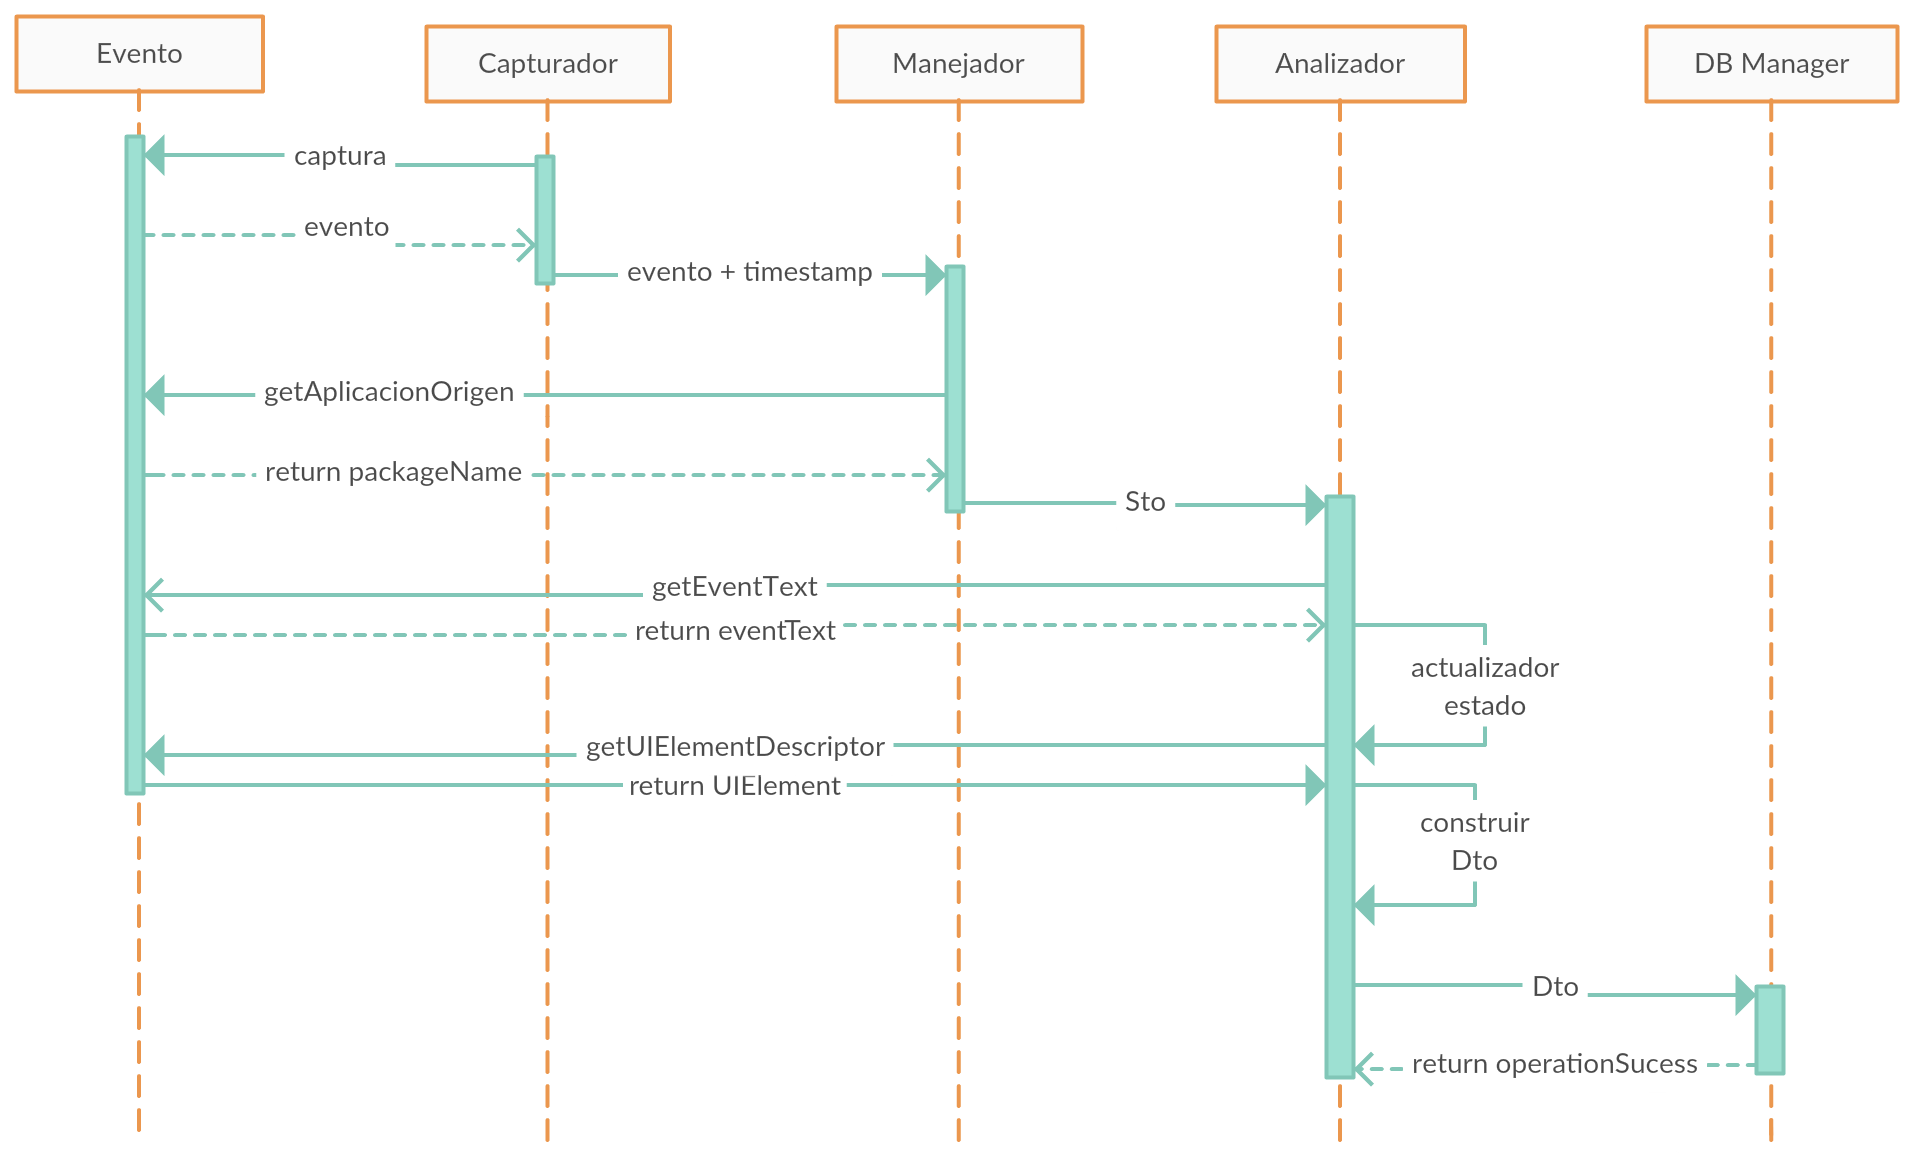
\includegraphics[scale=0.22]{pictures/secuencediagrams/diagrama_seq_flujo.png}
  \end{center}
  \caption[Diagrama de secuencia]{Diagrama de secuencia habitual del sistema.}
    \label{fig:LandscapeFigure}
\end{figure}
%\end{landscape}
\subsection{Conclusiones del análisis}
De esta forma, planteamos una arquitectura inicial dividida en capas, donde cada una está pensada para realizar una tarea simple y atómica. 
\newline \newline 
Se ha ideado esta arquitectura con la idea en mente de que sea un proyecto fácilmente ampliable, es decir, que el esfuerzo que conlleve añadir una nueva funcionalidad (por ejemplo, añadir una nueva app a la batería de aplicaciones a escuchar) tenga un impacto mínimo en el código y no implique grandes esfuerzos ni comunicaciones. 
\newline \newline 
Así, si estamos persiguiendo la idea de recolectar un determinado número de aplicaciones lo suficientemente grande como para poder conformar un perfil de usuario completo, veraz y objetivo, para añadir una aplicación al sistema de escucha únicamente deberemos implementar su analizador, puesto que el resto de componentes lo único que hacen es filtrar y conformar la información para esta capa. 
\newline \newline 
Con esta arquitectura conseguimos entonces el objetivo de que añadir aplicaciones para recolectar sus datos sea relativamente sencillo y lo único que hay que hacer es añadir código, sin tener que modificar la implementación existente. 
% -------------- %
% --- DISEÑO --- %
% -------------- % 
\chapter{Diseño}
En este capítulo se detalla el resultado de las sucesivas iteraciones sobre la etapa de diseño. A partir de los requisitos se ha estudiado el problema y planteado una arquitectura que nos permitirá guiar la implementación de los casos de uso. Se pretende obtener una arquitectura limpia y organizada de manera que permita la mantenibilidad del proyecto y una modificación mínima y eficaz. 
\section{Arquitectura}
A la hora de plantear nuestra arquitectura el primer paso será conocer la propia arquitectura de Android, por ello, en la siguiente sección estudiaremos como está planteado el sistema sobre el que nos basamos y en base a ese conocimiento tomaremos unas decisiones de diseño que nos ayudarán a componer la arquitectura final. 
\subsection{Decisiones de diseño}
Si nos fijamos en la siguiente figura vemos como Android se asienta en una modificación del Kernel de Linux sobre el que se van abstrayendo capas en las que cada una emplea los servicios que provee la capa inmediatamente inferior. 
%%% ------ 
\begin{figure}[H]
	\begin{center}
		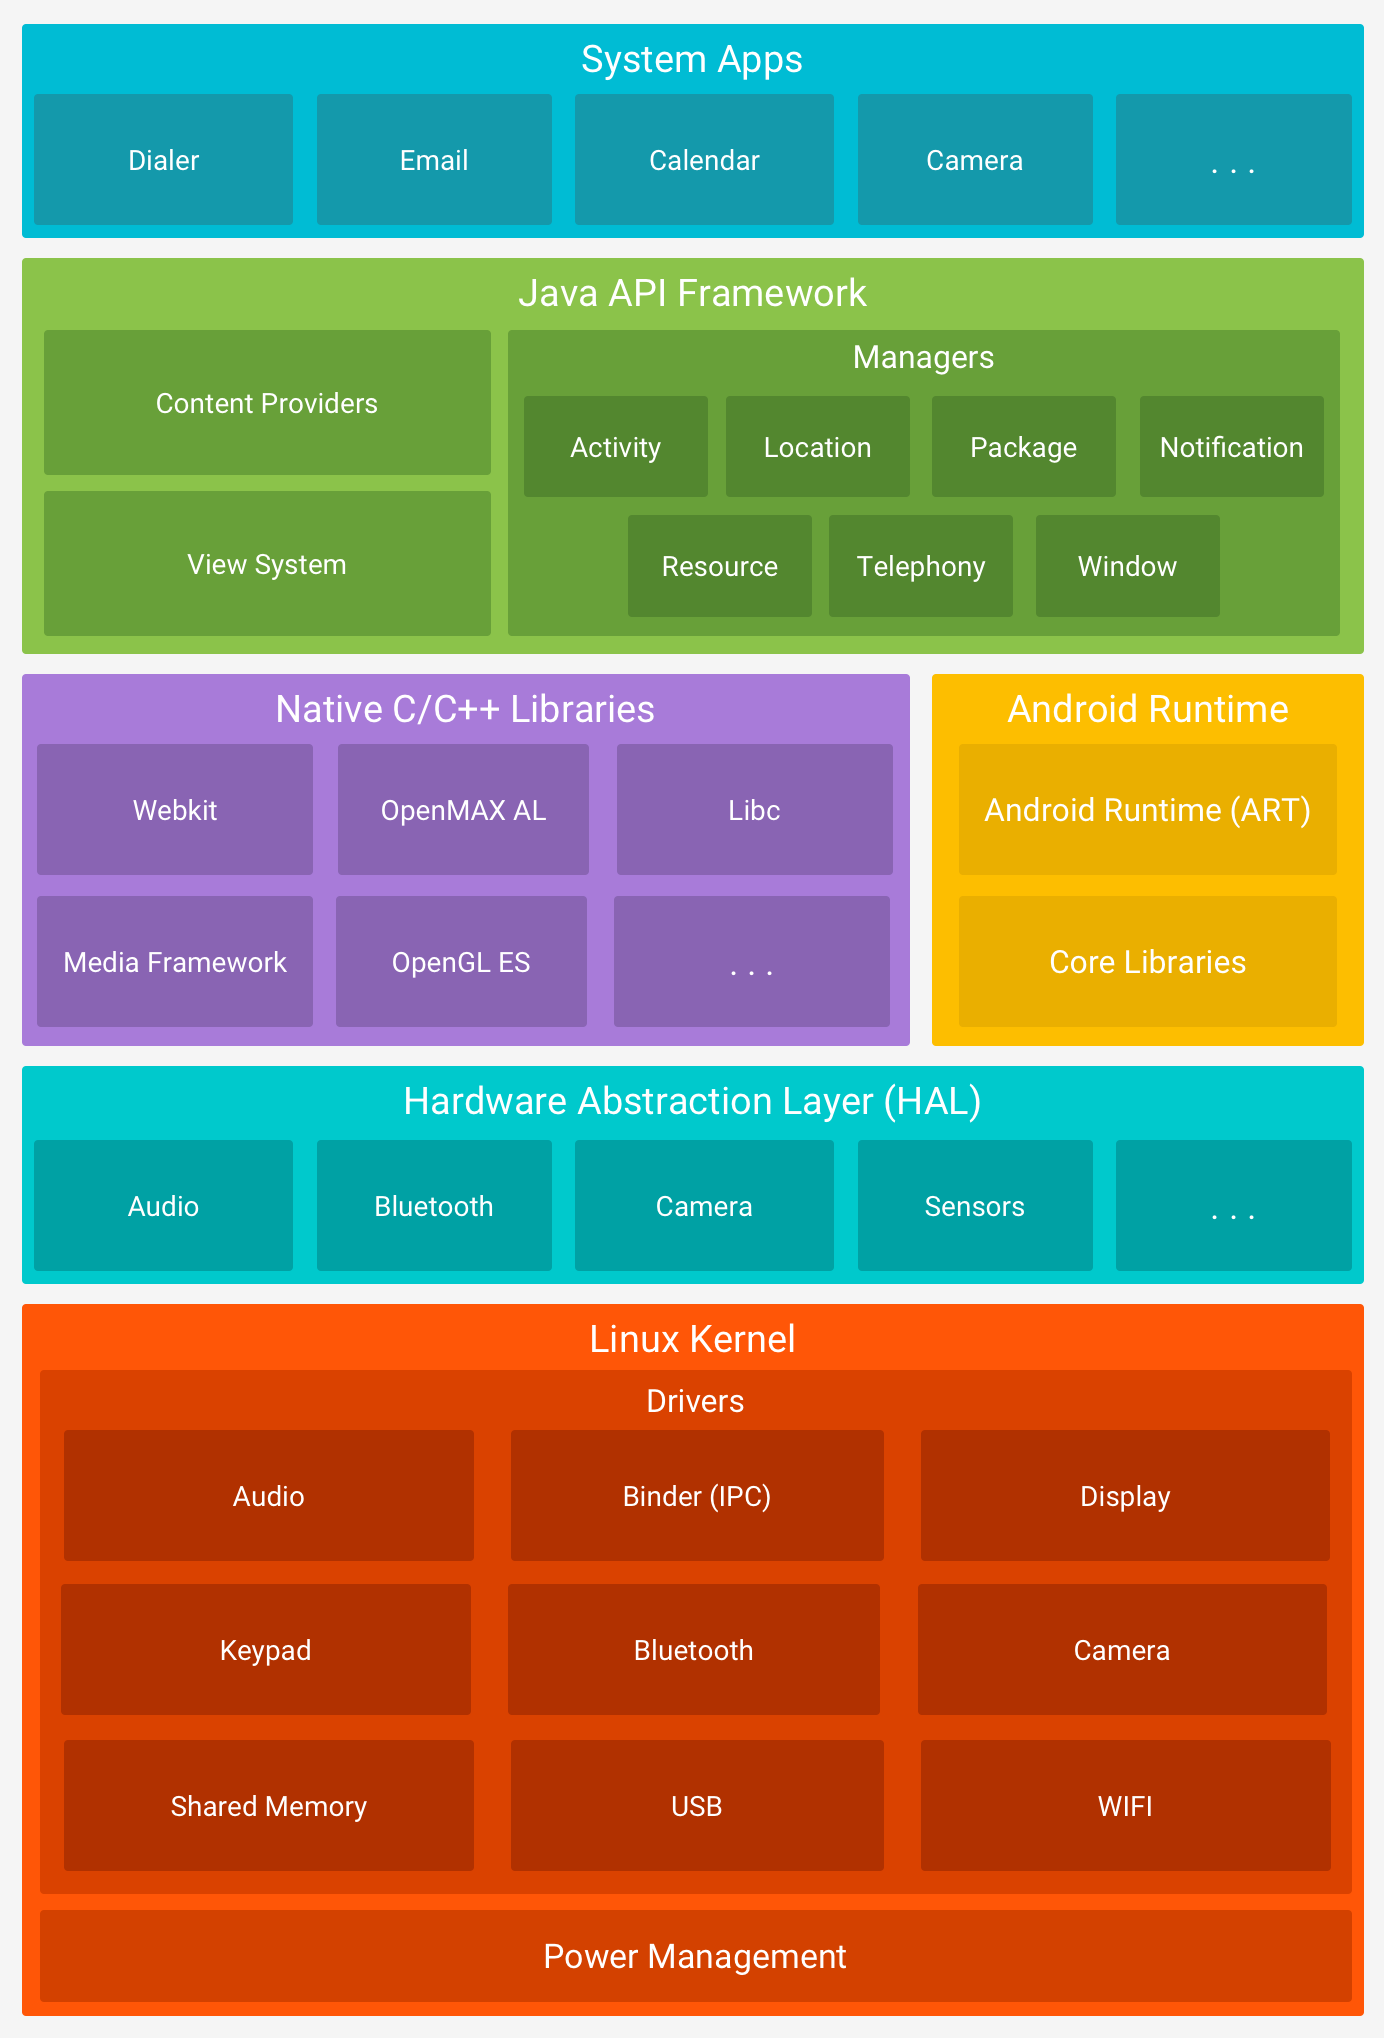
\includegraphics[scale=0.15]{pictures/architecture/android_stack.png} % include ./img/imagen.[pdf|png|jgp] si es pdflatex o ./img/imagen.eps si es latex
	\end{center}
	\caption[Android stack]{Arquitectura por capas de Android.}
\end{figure}
%%% ------
Así, como base de la arquitectura tenemos una modificación del Kernel de Linux sobre la cual se implementa una segunda capa, de abstracción del hardware, que será la encargada de manejar y comunicarse con los periféricos del teléfono. Entendemos por periféricos lo habitual en estos entornos; sensores, antenas, emisores radio...). Sobre estas dos capas, que permiten una interfaz de acceso al dispositivo Hardware, tenemos las librerías de bajo nivel y el entorno de ejecución de android. 
\newline \newline
Si avanzamos un poco más vemos que en las dos últimas capas están relacionadas con una API Java que permite al programador implementar aplicaciones, usando a través de la api, todo la anteriormente expuesto. 
\\
%%% ------ 
\begin{figure}[H]
	\begin{center}
		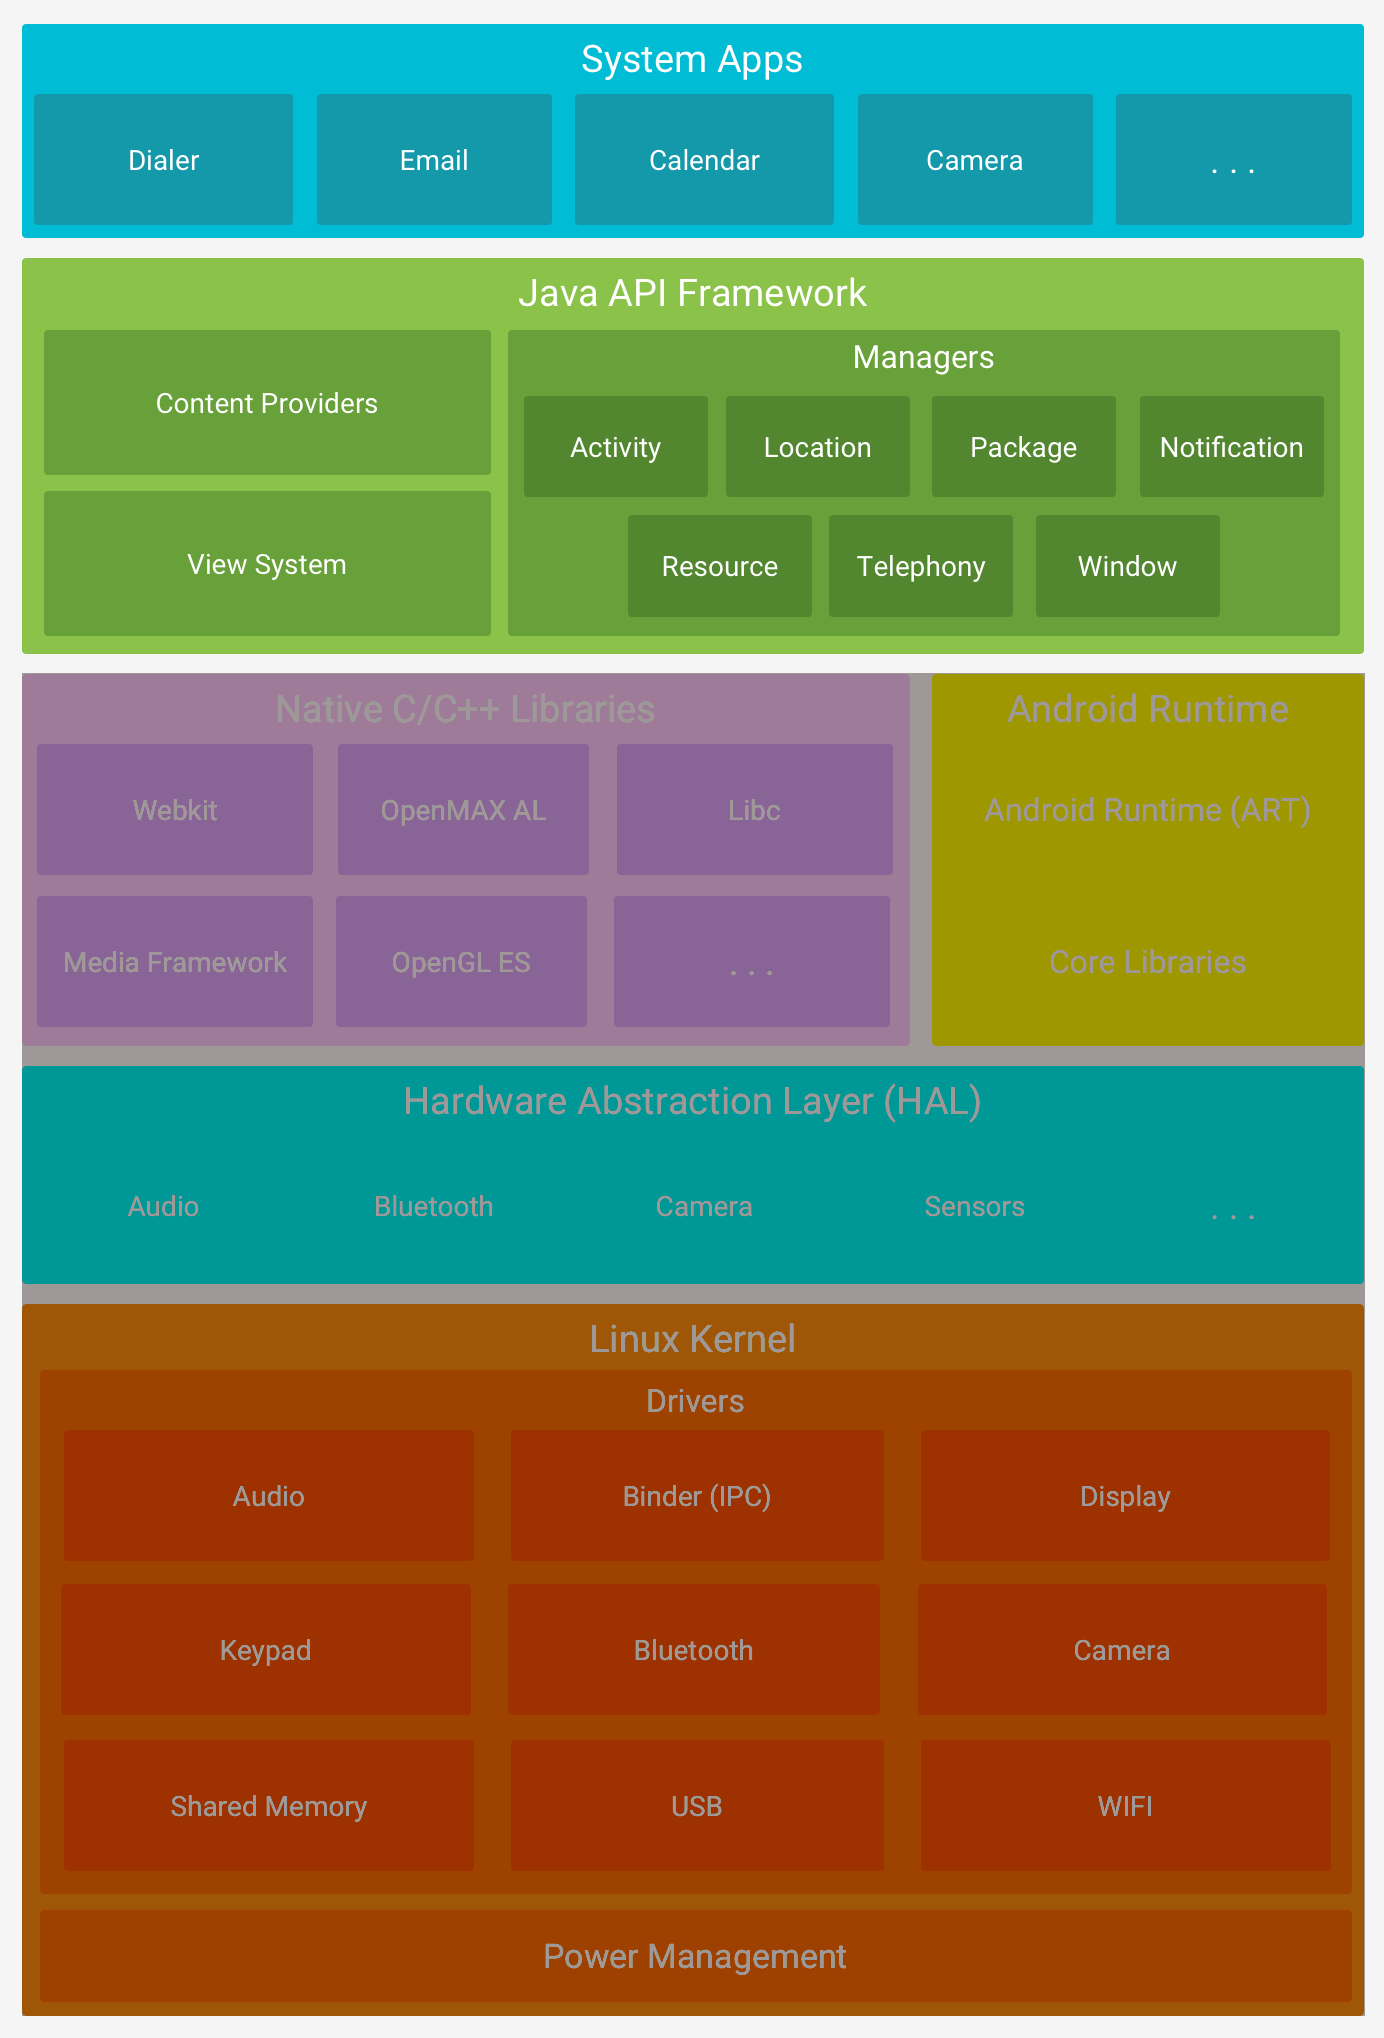
\includegraphics[scale=0.2]{pictures/architecture/android_stack_used.png} 
	\end{center}
	\caption[Detalle del Android Stack]{Márgenes del sistema}
\end{figure}
%%% ------
Estas dos últimas capas serán en las que se situará nuestra arquitectura. Además será conceptualmente parecida puesto que como hemos visto, Android dispone de un sistema organizado por capas, algo bastante lógico y habitual en los sistemas software, y nuestro objetivo por tanto debe ser separar funcionalidades y agruparlas bajo este patrón.
\newline
\newline
Teniendo este concepto claro, nos fijaremos en la publicación de Robert C. Martin, Clean Architecture, en la que se plantea el concepto de Arquitectura Limpia, sin ser más que una serie de condiciones que debe cumplir una arquitectura para que se la considere ”clean". Nos encontramos entonces con una serie de reglas, cuyo cumplimiento ayuda a diferenciar y dividir el software en capas, obteniendo además un software independiente de elementos externos (como la ui, frameworks y bases de datos), testeable y mantenible. 
\newline
\newline
En esta publicación nos encontramos con que una arquitectura debe partir de las entidades (entities). Estas entidades no son mas que las implementaciones sencillas de clases Java. 
\newline
\newline
Estas clases permitirán instanciar objetos que reprensentarán a los actores principales de la lógica de negocio. Por tanto POJOS (Plain Old Java Object) y Dtos (Data Transfer Objects) se verán incluidos en esta capa. 
%%% ------ 
\begin{figure}[H]
	\begin{center}
		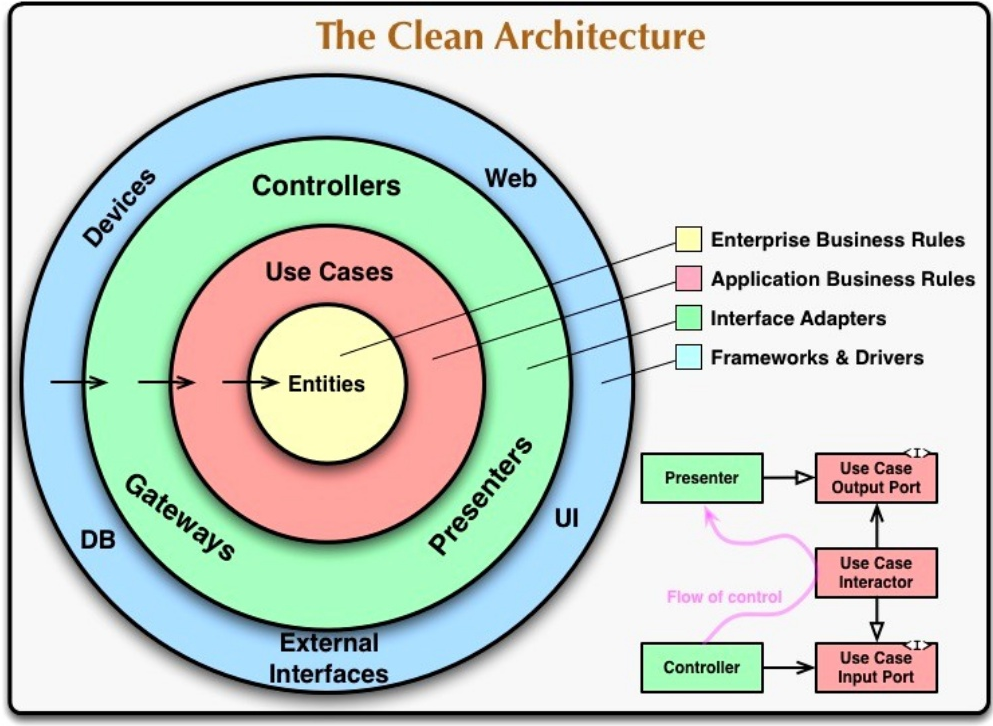
\includegraphics[scale=0.3]{pictures/architecture/android_architecture.png} 
	\end{center}
	\caption[Clean Architecture]{Arquitectura clean}
\end{figure}
%%% ------ 
Los casos de uso (use cases) están muy relacionados con las entidades, puesto que implementarán la lógica de negocio del sistema, orquestando y orientando el flujo de datos del sistema. 
\newline
\newline
La capa de los Interface Adapters realiza la conversión de los datos de manera que se puedan comunicar los niveles superiores con los casos de uso y entidades (en MVC corresponde a los Controladores, MVVP al presenter... etc). 
\newline
\newline
En la última capa y más externa, Frameworks and Drivers, residen las plataformas y herramientas externas, donde se incluye la interfaz de usuario, web... 
\subsection{Arquitectura a bajo nivel}
Una vez tenemos claro como está estructurado Android y los servicios que ofrece al desarrollador, debemos plantearnos cómo diseñar una aplicación que sea capaz de implementar estos servicios de accesibilidad para capturar, procesar y extraer la  información de los eventos que se generan, deberemos abstraernos del problema y ser capaces de, a partir de una vista general del sistema inferir las capas que finalmente nos guiarán la implementación. 
\newline
\newline
Así pues, en primer lugar situar nuestro sistema dentro del stack tecnológico de Android citado al principio de esta sección. 
\newline
%%% ------ 
\begin{figure}[H]
	\begin{center}
		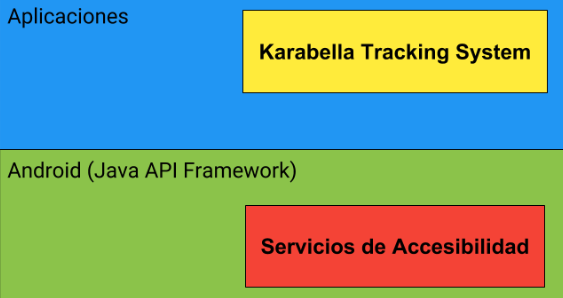
\includegraphics[scale=0.7]{pictures/architecture/arquitecturaGeneral01.png} 
	\end{center}
	\caption[Arquitectura dentro del android stack]{Arquitectura del sistema dentro del stack de Android.}
\end{figure}
Es natural esta clasificación puesto que el proyecto se basa en la implementación de los Servicios de Accesibilidad que Android dispone en de su API, gracias a mecanismos como la herencia y la implementación de interfaces. 
\newline \newline
Estos servicios de accesibilidad son la solución de Google para asistir y dar soportes a usuarios con diversidad funcional. Su naturaleza y comportamiento es lo que nos permite aprovechar estos servicios para obtener información de lo que hace el usuario. 
\newline \newline
Se comporta además como cualquier otro servicio de Android, (es decir, procesos ideados para correr en segundo plano con un ciclo de vida prolongado en el tiempo). El Servicio de Accesibilidad se comporta como listener de Eventos de Accesibilidad, que lanzados por el sistema, son recogidos por la clase que implemente este servicio, donde son capturados y tratados como mejor convenga. Estos eventos serán, entonces, la unidad de información más básica que manejará nuestro sistema, pero a la vez la más compleja, dado que llevan dentro toda la información sobre la cual se construyen el resto de capas.
\newline \newline
Los eventos llevan consigo información sobre la interfaz de usuario, por ejemplo los eventos se lanzan cuando entra en foco un elemento (con la descripción del elemento, botones, entradas de texto, nombres de ventanas...). Nuestra solución pasa por extraer la información de esos eventos y procesarla. 
\newline \newline
Dado que estos eventos pueden ser capturados por Eventos de Accesibilidad, nuestro sistema contará con un servicio que lo implemente y que realiza esta captura, este será un elemento fundamental en la arquitectura puesto que será la base sobre la que se asentarán el resto de elementos. 
\newline \newline 
De esta forma, y siguiendo las líneas definidas, obtenemos una arquitectura detallada en el siguiente diagrama. 
%%% ------ 
\begin{landscape}
\begin{figure}[htb]
	\begin{center}
		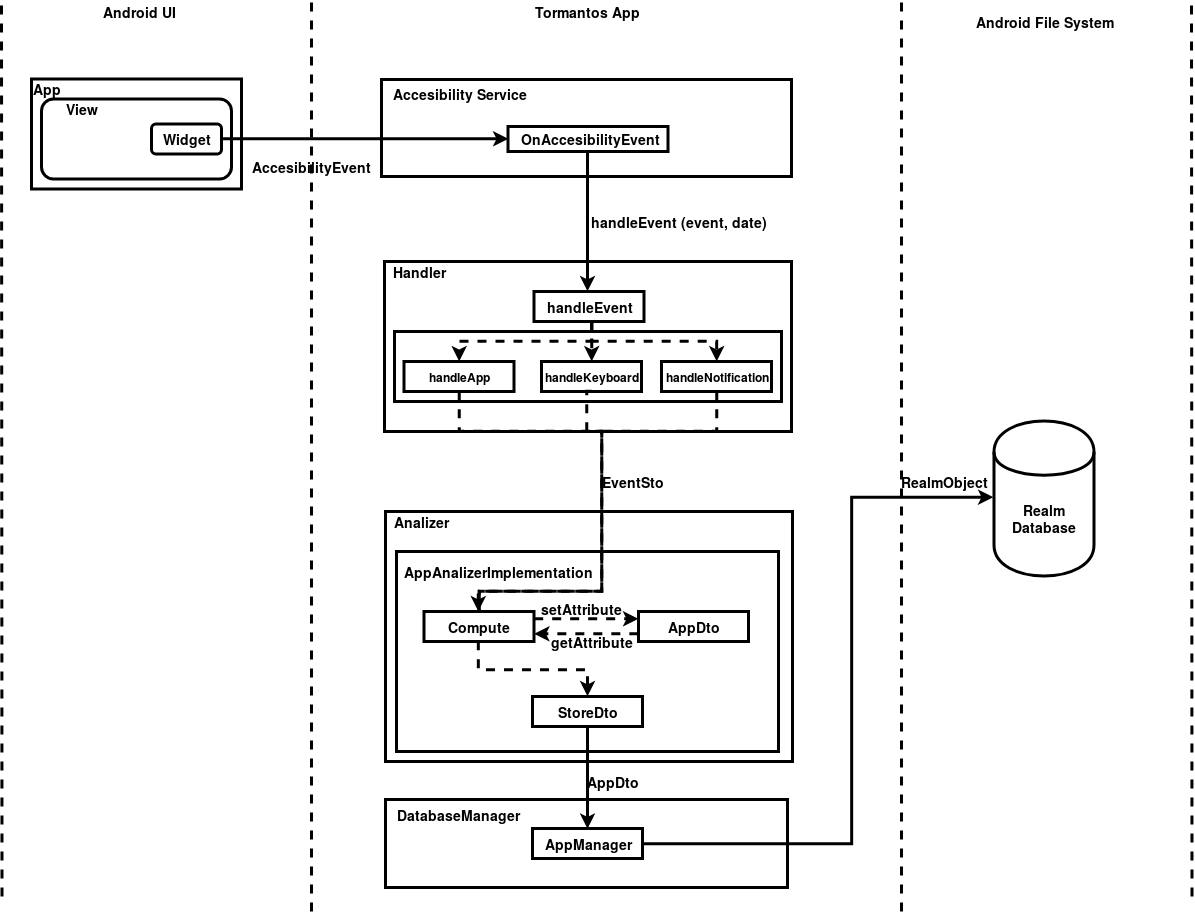
\includegraphics[scale=0.45]{pictures/architecture/lowLevel/TFG_ArquitecturaBajoNivel01.png} 
	\end{center}
	\caption[Arquitectura general del sistema]{Arquitectura general del sistema}
\end{figure}
\end{landscape}

%%% ------ 
Donde la interfaz de usuario (UI) genera eventos de accesibilidad. Estos eventos, como ya se ha comentado, están asociados a cada acción que el usuario realiza con el teléfono sobre la interfaz. Será la implementación del evento de accesibilidad (Accesibility Service) el que nos permita capturarlos. 
\newline
\newline
Este servicio se encargará de capturar los eventos y mandarlos hacia el Manejador de Eventos (EventHandler), este manejador será el encargado de clasificar y procesar los eventos en función de la información que traigan consigo. 
\newline
\newline
El manejador de eventos es un componente crucial del sistema. Será el encargado de, en función de la aplicación origen del evento, mandarlos a un analizador u otro. Además, no sólo se centra en los eventos de las aplicaciones que estamos escuchando, si no que mantiene un control sobre componentes del sistema como el teclado o las notificaciones. 
\newline 
\newline 
Estos eventos de teclado son cruciales para algunos analizadores, nos permitirán controlar la entrada de texto del usuario. Por lo tanto el manejador deberá mantener la información de la aplicación que se está escuchando en cada momento, y en función de ello, y junto al evento de teclado, llamar al analizador oportuno para que realice la tarea correspondiente. 
\newline
\newline
Siguiendo con el resto de componente, nuestro sistema cuenta con una interfaz Analyzer, con tantas implementaciones 
 aplicaciones estemos monitorizando. Procesarán el evento de accesibilidad y lo encapsularán en una unidad de datos que será pasada a la capa de persistencia, formada por un Manager de objetos. Este Manager será la entidad responsable de persistir en una base de datos local los datos generados por el sistema, además de realizar el dump de los datos cada vez que proceda. 
\newline
\newline
Con el GPS y los sensores la historia es diferente, puesto que la escucha de los mismos está ligada a la implementación de sendos listeners dentro de un servicio en segundo plano. Este servicio por tanto, lanzará tantos dos listeners, por un lado, el listener de la localización y por otro, un listener de los sensores que están incluidos en el terminal. Cada vez que se detecten cambios en los valores del GPS o los sensores, se empaquetará la información en un Dto y se llevará al DBManager para que la persista.
\newline 
\newline 
En la parte del DataManager tendremos entonces la implementación de las operaciones de guardado y recuperación de la base de datos. Esta implementación ha ido cambiando a lo largo del desarrollo. En un principio había tantas implementaciones del manejador como entidades de datos estaba manejando la aplicación. Con el tiempo esto cambió para encontrarnos una única clase DBManager que, de forma anónima, maneja los objetos que los analizadores le comunican. 
\newline \newline 
Esto se ha hecho persiguiendo el objetivo de parametrizar lo máximo posible las implementaciones de las clases participantes en el sistema. El DBManager recibirá objetos de tipo Dto, los cuales extienden de RealmObject (como se verá en el siguiente capítulo). Así, DBMaganer lo único que conoce de los objetos que maneja es que son instancias de tipo RealmObject, con lo cual nos evita duplicar código y nos aporta flexibilidad y comodidad a la hora de modificar o ampliar el proyecto. 
\newline \newline
De esta manera nos encontramos con 4 capas separadas por funcionalidad y con independencia lógica entre ellas, puesto que cada una está consagrada a una tarea particular (servicios de escucha, manejar eventos, computarlos, persistirlos). 
\newline \newline
La lógica de negocio del sistema se encuentra, sin duda, en las capas del manejador y analizador, donde deberemos de echar un esfuerzo de implementación considerable para manejar todo el flujo de información. 
\newline \newline 
\subsection{Diagrama de clases}
Por un lado, tenemos dos servicios en la aplicación, el primero, \textbf{AccessibilityServiceImpl}, implementa un Servicio de Accesibilidad, nos permitirá capturar los eventos generados por la interfaz al interactuar el usuario con la misma.
\newline \newline
El segundo, \textbf{SensorListenerService}, implementa dos interfaces, por un lado \textbf{LocationService}, para la captura de la localización GPS, y por otro, \textbf{SensorEventListener}, para la captura de los valores de los sensores de ambiente del teléfono. 
\newline \newline
Este servicio es independiente a manejadores, analizadores y demás elementos del sistema. Cuando detecten un cambio en los valores del gps o los sensores, lo almacenarán en el Dto correspondiente (LocationDto para la localización y Sensor Dto para los sensores) llamando para ello al DBManager. 
\newline \newline
Siguiendo con el \textbf{servicio de accesibilidad}, la implementación de esta interfaz nos permite, como ya se ha dicho, capturar los gestos que realiza el usuario en la pantalla. Son los \textbf{eventos de accesibilidad} los que nos aportan esa información. 
\newline \newline
Una vez que este servicio de accesibilidad captura esos eventos, se comunica con el manejador, que deberá comprobar el nombre del paquete que originó el evento para llamar a la implementación del analizador correspondiente. Este analizador será el responsable de extraer la información del evento y darle sentido al carro de datos que entrará en el sistema. 
\newline \newline
De esta manera, nos encontramos tantos analizadores como aplicaciones queremos escuchar. Al tratarse de la implementación de una interfaz, todas las implementaciones deberán contar con los métodos compute, para extraer y darle significado a la información recogida, y store, para persistir la instancia del objeto capturado en la base de datos. 
\newline \newline
Los objetos en los cuales almacenamos la información están asociados a los analizadores, y dada la naturaleza de la aplicación, habrá tantos como aplicaciones queramos escuchar, puesto que los atributos deben adaptarse a la naturaleza de la misma. 
\newline \newline
De cualquier modo, para mejorar la compresión del diagrama, se han agrupado las clases del analizador en 5 paquetes. A saber, Browsing, Social, System, Communication y Messaging. Dentro de ellos los atributos de cada dto son similares unos a otros, puesto que la naturaleza de las aplicaciones que se incluyen en cada uno son similares. 
\newline \newline
Teniendo este diagrama en mente, y conociendo como está estructurada la arquitectura y su implementación, veamos como se ha realizado la misma. 
%%% ------ 
\begin{landscape}
\begin{figure}[htb]
\begin{center}
		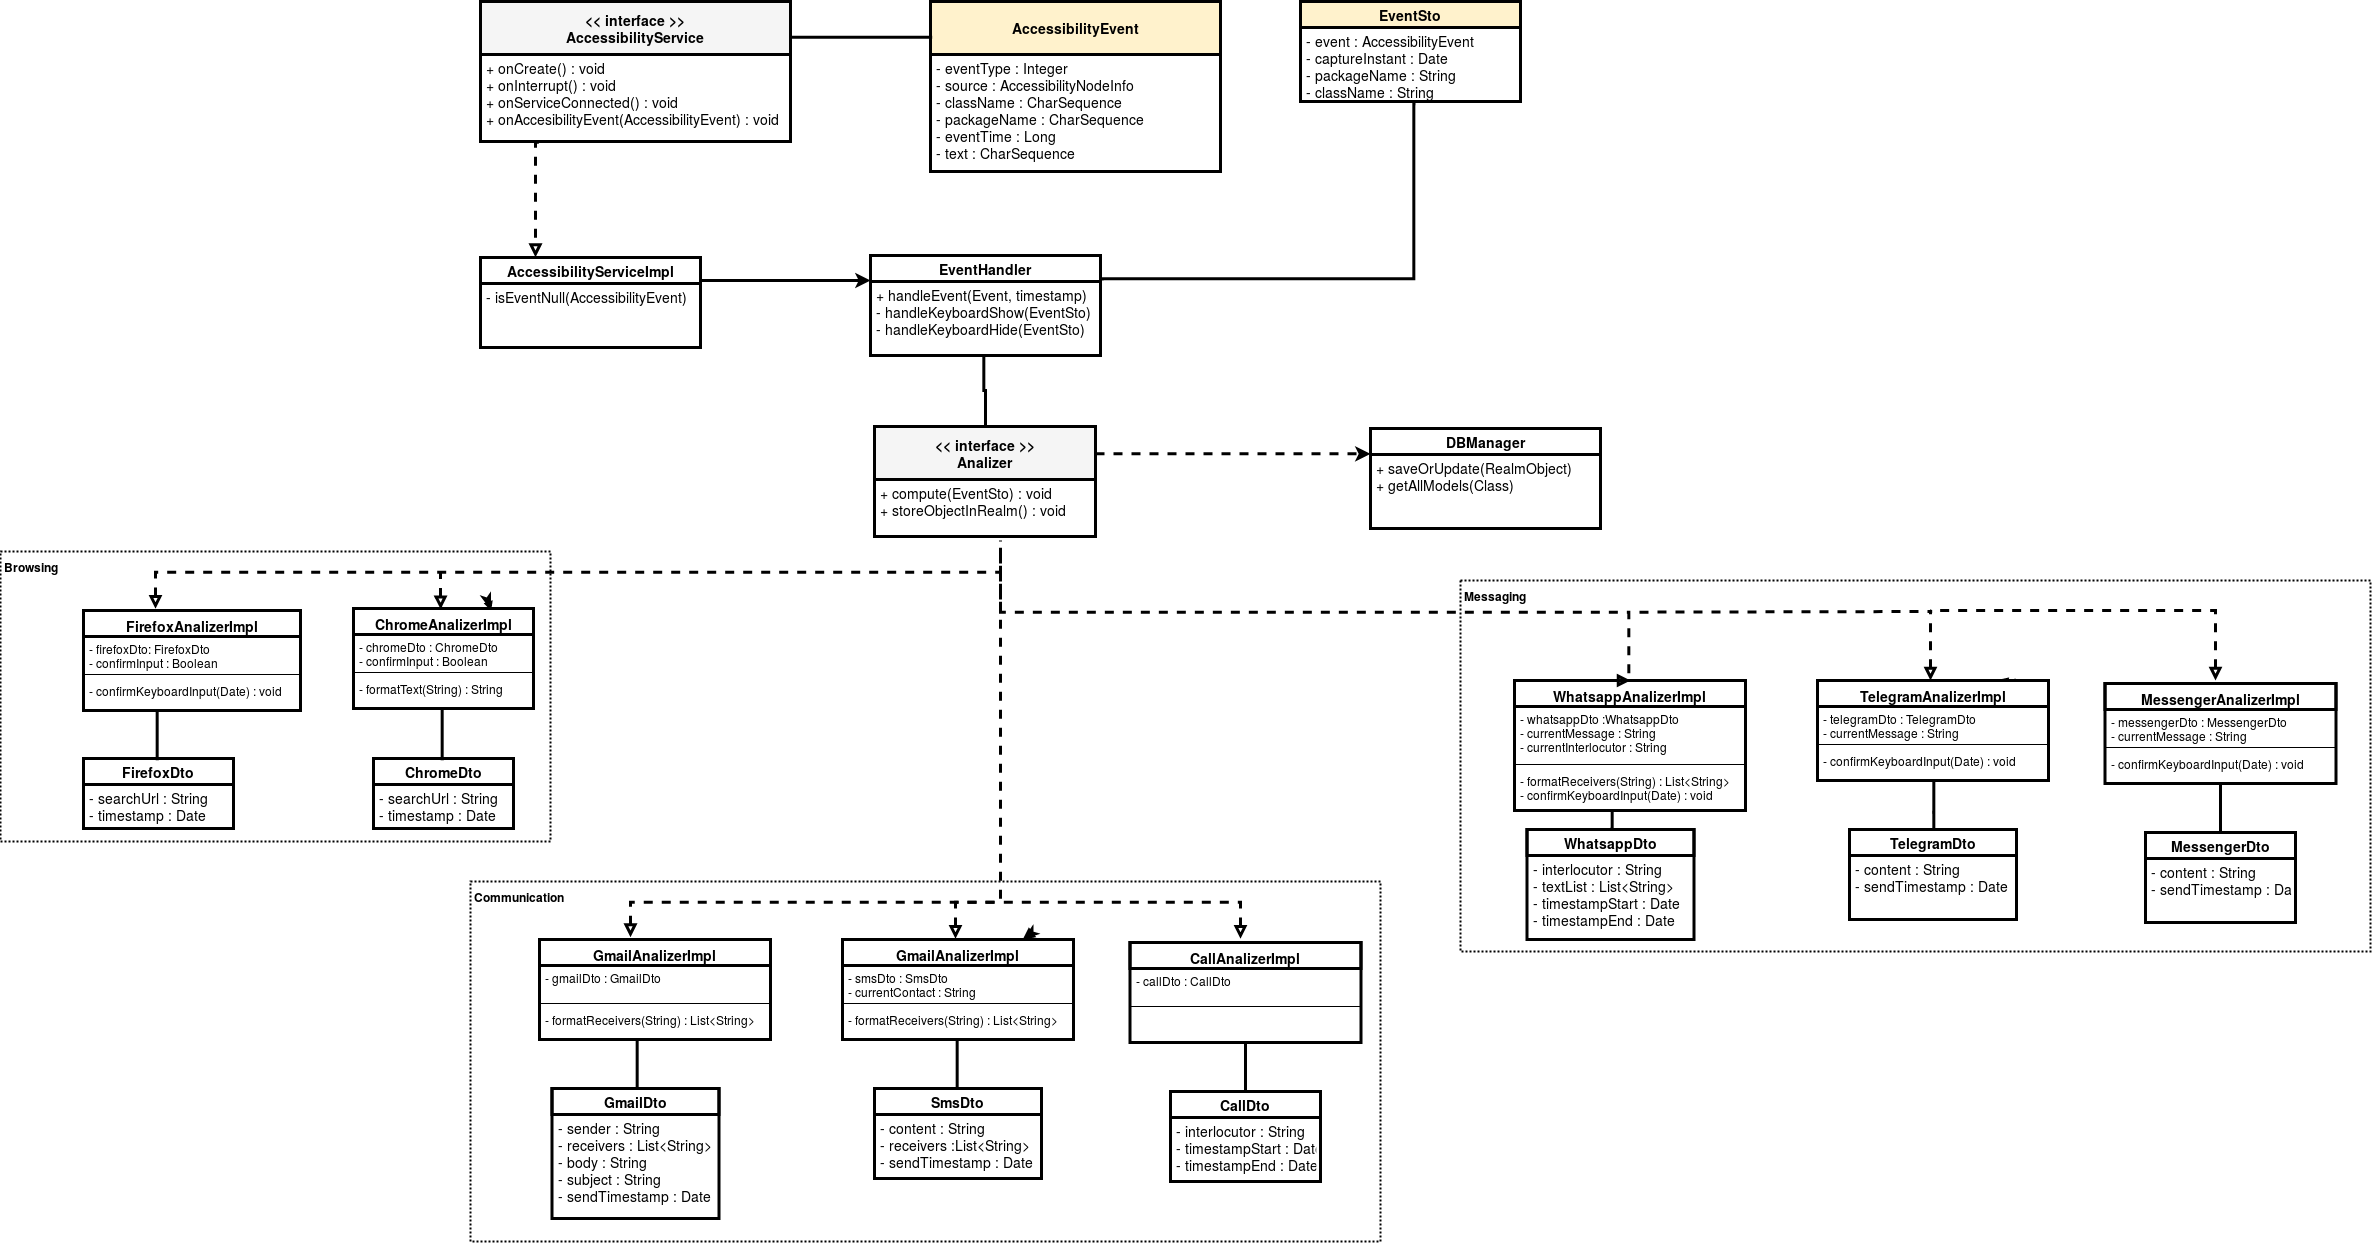
\includegraphics[scale=0.32]{pictures/classDiagram/classDiagram.png} 
%	\end{large}
	\caption[Diagrama de clases de la aplicación]{Diagrama de clases de la aplicación}
	\end{center}
\end{figure}
\end{landscape}
\subsection{Conclusiones del diseño}
A lo largo de este capítulo hemos planteado una arquitectura para nuestro sistema. Con la idea de plantear un diseño eficiente y dirigido, hemos empezado por ver cómo está planteado el propio sistema Android con sus frameworks y aplicaciones, pasando por la definición del \textit{clean architecture}, con la idea de aplicar el mismo concepto a nuestro sistema. 
\newline \newline 
El resultado es una arquitectura divida en capas, donde se ha pretendido aislar lo máximo posible una de otra, y donde una capa sólo conoce la existencia de la inmediatamente inferior, para poder comunicarse con ella mediante mensajes que, en este caso, contienen instancias de objetos. 
\newline \newline 
Además, se ha planteado el analizador como una interfaz bajo la premisa de poder añadir nuevas aplicaciones a la batería ya existentes, con, en vistas a un futuro, completar cada vez más nuestro sistema. Por ello, si se desea entonces crear nuevos analizadores, bastará con implementar la interfaz planteada y añadir su detección en el manejador. 
\newline \newline 
El resultado es una arquitectura flexible, mantenible y sencilla. 
\chapter{Implementación y desarrollo}
Durante el siguiente capítulo veremos documentada la lógica que sigue la aplicación, centrándonos en el servicio de escucha en segundo plano, responsable de capturar los datos del usuario en cada una de las aplicaciones que nos permitirán conocer su perfil completo en cada una de sus facetas. Recordemos, comunicación, mensajería, navegación, redes sociales y el plano físico mediante los sensores. 
\newline \newline 
En primer lugar, debemos conocer los objetos y los datos con los que estamos trabajando. A lo largo del proyecto hemos citado en innumerables ocasiones los eventos de accesibilidad, pero el lector aún no conoce su forma, su contenido ni cómo se generan. También se adjuntará una descripción de los objetos Dto donde almacenaremos la información, con el fin de situar al lector dentro del marco en el que se ha realizado la implementación del proyecto. 
\section{Accessibility Events}
A lo largo del documento, hemos venido hablando una y otra vez de los eventos de accesibilidad. Ya es hora de que el lector los conozca y vea en que consisten realmente y cómo son generados. 
\newline \newline 
Sin duda, \textit{ver} los eventos de accesibilidad es de gran ayuda, tanto para el lector como para el programador. Por ello, tenemos un método que nos permite mostrar por consola la información que viene asociada al evento de accesibilidad. 
\newline \newline 
Así, si el desarrollar desea capturar una aplicación, deberá conectar su teléfono al IDE e interactuar con el dispositivo mientras se muestran por pantalla estos eventos. De esta manera podrá ver los eventos generados, con la información que los acompaña. 
\newline \newline 
Al mostrar por consolas los eventos, mostramos seis atributos clave, con los que trabajaremos a lo largo de la implementación. 
\begin{itemize}
	\item \textbf{Type}: Describe el tipo de evento. Tenemos una enorme cantidad de tipos, algunos de ellos, por ejemplo son \textit{TYPE VIEW CLICKED}, representa el hecho de pulsar sobre una vista, botón, etc. \textit{TYPE NOTIFICATION STATE CHANGED}, el evento que lanza una notificación al mostrarse, \textit{TYPE WINDOW STATE CHANGED}, es el evento que se genera cada vez que cambia el contenido de la pantalla del usuario, y así, un largo etc. 
	\item \textbf{EventId}: Es el valor entero del EventType. 
	\item \textbf{Class}: Se trata del nombre de la clase del elemento de la interfaz que generó el evento. Podemos tener de todo, widgets  coom el EditText, ImageButton, LinearLayout, vistas como el ViewGroup, y un largo etc.
	\item \textbf{Package}: El nombre del paquete de la aplicación que generó el evento. Esto nos permitirá identificar las aplicaciones que dan lugar a los eventos y por tanto, será de gran ayuda para el manejador a la hora de discernir a qué analizador enviar el evento. 
	\item \textbf{Time}: El instante en el que se generó el evento. 
	\item \textbf{Text}: El texto que acompaña al evento. Aquí puede haber de todo, desde los placeholders que acompañan a las entradas de texto, el propio texto que escribe el usuario, el nombre de una ventana, etc. 
\end{itemize}
Conociendo ya los atributos que vamos a manejar, veamos un ejemplo de una salida por consola. 
\begin{verbatim}
D/Helper: [type] TYPE_VIEW_TEXT_CHANGED 
[eventId] 16 [class] android.widget.EditText 
[package] com.whatsapp [time] 06/07/2018 19:51:25 
[text] Hola! Lector

D/Helper: [type] TYPE_WINDOW_STATE_CHANGED 
[eventId] 32 [class]  
[package] com.google.android.inputmethod.latin 
[time] 06/07/2018 19:51:25 
[text] Se han rechazado las alternativas

D/Helper: [type] TYPE_WINDOW_STATE_CHANGED 
[eventId] 32 [class]  
[package] com.google.android.inputmethod.latin 
[time] 06/07/2018 19:51:25 
[text] Mostrando teclado español (España) (QWERTY (Ñ))

D/Helper: [type] TYPE_WINDOW_STATE_CHANGED 
[eventId] 32 [class]
[package] com.google.android.inputmethod.latin 
[time] 06/07/2018 19:51:30 
[text] El teclado español (España) (QWERTY (Ñ)) está oculto

D/Helper: [type] TYPE_WINDOW_STATE_CHANGED 
[eventId] 32 [class] com.google.android.launcher.GEL 
[package] com.google.android.googlequicksearchbox 
 [time] 06/07/2018 19:51:32 
 [text] Aplicaciones
 
D/Helper: [type] TYPE_WINDOW_STATE_CHANGED 
[eventId] 32 [class] com.google.android.launcher.GEL 
[package] com.google.android.googlequicksearchbox 
[time] 06/07/2018 19:51:34 
[text] Pantalla de inicio 1 de 1

D/Helper: [type] 16384 
[eventId] 16384 [class] android.view.ViewGroup 
[package] com.google.android.googlequicksearchbox 
[time] 06/07/2018 19:51:35
[text] Pantalla de inicio 1 de 1

D/Helper: [type] TYPE_WINDOW_STATE_CHANGED 
[eventId] 32 [class] android.widget.FrameLayout 
[package] com.android.systemui 
[time] 06/07/2018 19:51:38 
[text] Pantalla de bloqueo.
\end{verbatim}
El output listado arriba se corresponde con la acción de enviar una cadena de texto a un contacto de Whatsapp y, mediante el botón de \textit{back}, navegar hacia la pantalla principal de la app, llegar a la caja de aplicaciones y volver a la pantalla principal. Una vez ahí se ha bloqueado el dispositivo. 
\newline \newline 
La gran complicación del proyecto consiste en la enorme cantidad de información que generan acciones que tenemos muy automatizadas como usuarios. Nuestro objetivo entonces consiste en poner orden a ese carro de datos. 
\newline \newline 
Para ello, durante el proceso de implementación, cada vez que nos enfrentamos a una nueva captura, debemos debugguear los servicios generados (con outputs similares al de arriba) y estudiarla hasta detectar el patrón que se corresponde a la acción que queremos capturar (por ejemplo, la escritura en Whatsapp o una búsqueda Web). 
\newline \newline 
Una vez detectado este patrón, se debe implementar el analizador. En primer lugar, esta implementación consiste en imponer filtros y condicionales que descarten aquellos eventos que no son de nuestro interés. De esta manera, a la capa del analizador llegan únicamente los eventos asociados a la aplicación que queremos escuchar en ese momento. 
\newline \newline
Una vez hecho esto, se debe implementar el método \textit{compute} del analizador correspondiente. Sendos condicionales consiguen que en función del elemento de la interfaz donde fué originado el evento, consigamos leer la información del ellos y asociarla a los atributos del Dto donde guardaremos la información. 
\newline \newline 
De esta manera, detectando patrones, filtrando eventos y leyendo su información, conseguiremos imbuir información a los objetos dtos, los cuales usaremos para persistir el fruto de nuestra captura. 
\newline \newline 
En el proyecto se incluyen capturas de varias aplicaciones, veamos a continuación tres de ellas que, por su relevancia, consideramos interesantes estudiar en detalle. 
\section{Captura de Gmail}
En este apartado, y los que siguen, veremos los objetos destinados a guardar la información y los diagramas de actividad de tres aplicaciones clave para el perfilado del usuario, Gmail, Whatsapp y el navegador Chrome. Tienen como objetivo clarificar y documentar el flujo lógico que seguirá cada aplicación, durante el proceso de análisis y extracción del contenido de una cada de las aplicaciones propuestas.
\subsection{GmailDto}
El objeto donde guardaremos la información de captura se compone de los siguiente atributos; 
\begin{verbatim}
public class GmailDto extends RealmObject {
 	@PrimaryKey
    private String id;

    /** The mail sender */
    private String sender;

    /** The mail receivers */
    private RealmList<String> receivers;

    /** Mail subject */
    private String subject;

    /** Mail content */
    private String body;

    /** When the mail was sended */
    private Date timestamp;
 	
 	// -- getters and setters   
}
\end{verbatim}
En primer lugar nos encontramos un identificador. Esto es necesario en tanto el cuanto el objeto herede de RealmObject. Este RealmObject es propio del framework Realm, una base de datos orientada a objetos que destaca por su rapidez. La veremos más adelante en la sección de librerías de terceros. 
\newline \newline 
Empezando ya con los atributos relevantes para la captura, por un lado tenemos un atributo \textbf{sender}, destinado a almacenar el emisor del correo. Se podría pensar que es obvio que el que manda un correo es el usuario del teléfono, pero hoy en día es habitual que una persona tenga varias cuentas de correo, por ello almacenaremos en este atributo cuál de ellas elige. 
\newline \newline 
El atributo \textbf{receivers} consiste en una lista (del framework Realm) de Strings. El motivo de que este atributo sea una lista y no un String sin más es sencillo, y es que un correo puede tener varios destinatarios. Almacenaremos como elementos independientes del array cada dirección de correo que el usuario escribe. 
\newline \newline 
El atributo \textbf{subject} tiene como destino almacenar el asunto del correo. Lo mismo ocurre con \textbf{body}, cuya aplicabilidad no es otra que guardar el cuerpo del mensaje en sí. 
\newline \newline 
Por último no encontramos con un atributo \textbf{timestamp} del tipo java.util.Date. Su propósito es aportar un contexto temporal sobre el momento del día en el que el usuario se dedica a mandar correos electrónicos. 
\subsection{Diagrama de actividad}
En la siguiente figura se documenta el proceso que lleva al registro de un correo mandado por el usuario a través de la aplicación de GMail. Se ha organizado el diagrama por niveles, desde la capa más externa de la aplicación hasta la capa de persistencia, así se puede observar tanto el camino recorrido por los datos como el procesamiento de la información en cada nivel.
%%% ------ ACTIVIDAD GMAIL 
\begin{landscape}
\begin{figure}[htb]
	\begin{center}
		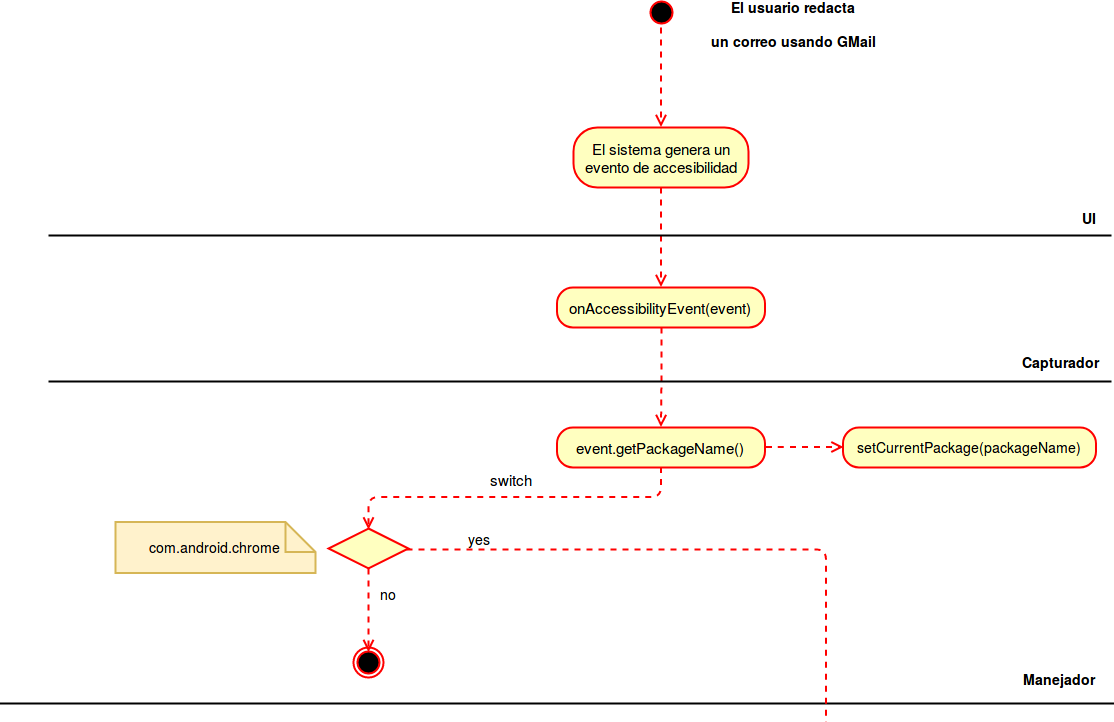
\includegraphics[width=1.1\textwidth]{pictures/activity/gmailActivityDiagram1.png} 
	  \caption[Diagrama actividad GMail (1)]{Diagrama de actividad de captura de un correo redactado con GMail (1).}
	  \label{fig:Diagrama actividad GMail (1)}
  	\end{center}
\end{figure}
\end{landscape}
\begin{landscape}
\begin{figure}[htb]
	\begin{center}
		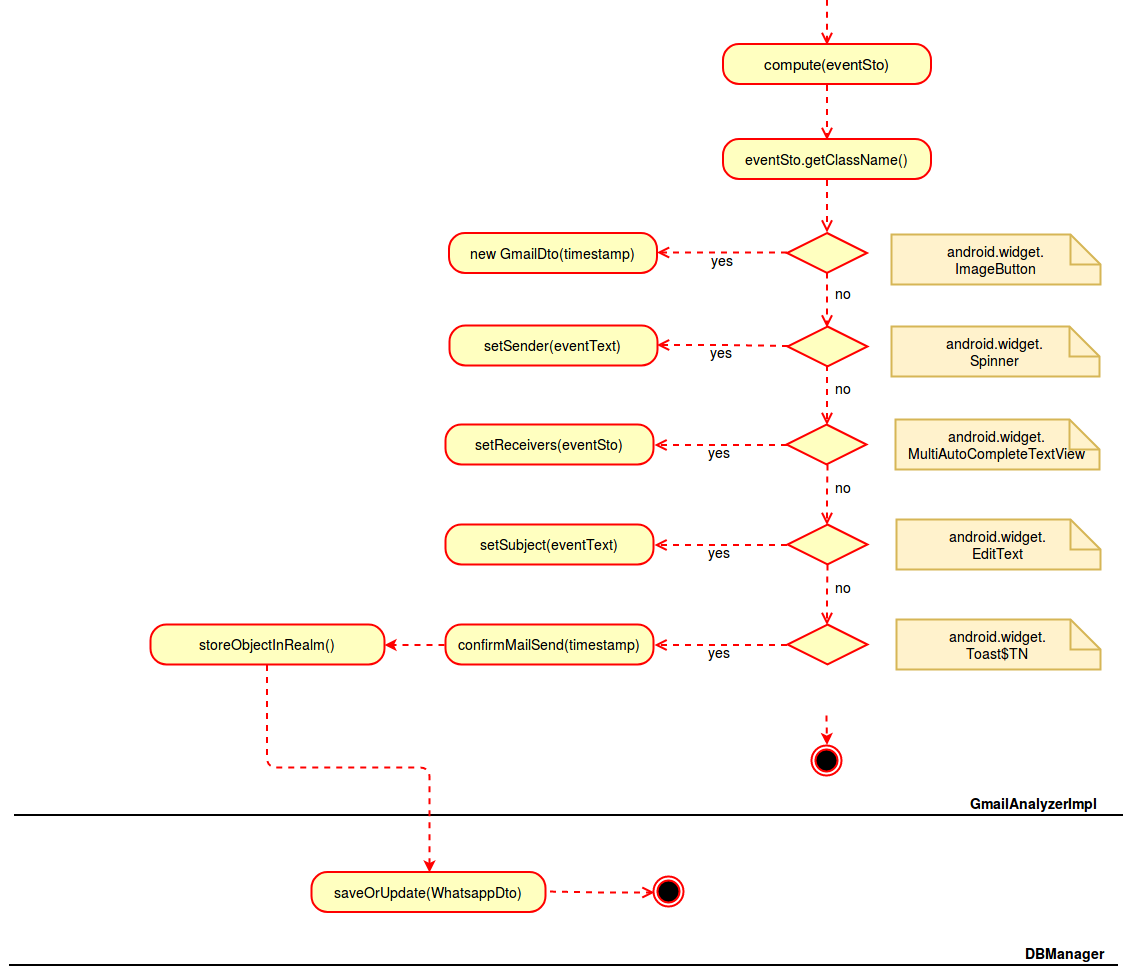
\includegraphics[width=1.1\textwidth]{pictures/activity/gmailActivityDiagram2.png} 
	  \caption[Diagrama actividad GMail (2)]{Diagrama de actividad de captura de un correo redactado con GMail (2).}
	  \label{fig:Diagrama actividad GMail (2)}
  	\end{center}
\end{figure}
\end{landscape}
%%% ------  /ACTIVIDAD GMAIL

 Así, podemos desglosar el proceso en los siguientes puntos, explicando que se hace en cada componente. 
\begin{itemize}
\item \textbf{UI}. En primer lugar, el usuario inicia la actividad al lanzar la aplicación de GMail e interactuar con su interfaz. Esta acción provoca que se lance un evento de accesibilidad por cada elemento gráfico que compone la pantalla. 
% -- item CAPTURADOR
\item \textbf{Capturador}. Actúa como un listener de eventos de accesibilidad, de esta manera está a la escucha de todos los eventos producidos por el sistema, los cuales recoge y junto a la marca horaria del instante de la captura, se lo transfiere al manejador. 
% -- item MANEJADOR
\item \textbf{Manejador}. Comprueba el nombre del paquete que trae consigo el evento, asociado a la aplicación que le dió lugar. En este caso, si el nombre del paquete de la aplicación coincide con el de GMail, \textit{com.google.android.gm}, invoca al analizador de gmail y le delega el evento. 
% -- item ANALIZADOR
\item \textbf{Analizador}. Este es nivel con más carga, puesto que debe comprobar cada evento recibido buscando los componentes de la interfaz conocidos, es decir, aquellos en los que sabemos que se vierte la información que compone el correo. Estos elementos son; 
\begin{itemize}
% -- new subitem
\item \textit{Widget Image Button}. Es el botón de editar que figura en la esquina inferior derecha de la interfaz. 
 	\begin{figure}[htb]
		\begin{center}
     		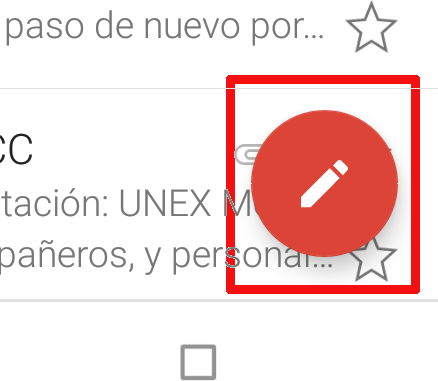
\includegraphics[scale=0.2]{pictures/IRL/GMail/dashboard_gmail_nuevo_correo_cutted.png}
	    	\caption{Android Image Button}{Elemento botón que lanza la creación de un nuevo correo}
    		\label{fig:Android Image Button}
		\end{center}
	\end{figure}
\newline
Al pulsarlo el usuario, el sistema lanza una nueva pantalla en la que redactará el correo. Con lo cual, la pulsación de este elemento de la UI nos inicia el proceso de captura poniendo a nuestro servicio un contenedor, donde compondremos la información del correo. 
\newline
\newline
Cada vez que se pulse este elemento se instanciará un nuevo GmailDto, con el que se trabajará durante el proceso de captura. 

% -- new subitem
\item \textit{Widget Spinner}. Se trata del campo donde aparece el emisor, es decir, el correo del usuario. 
 	\begin{figure}[H]
		\begin{center}
     		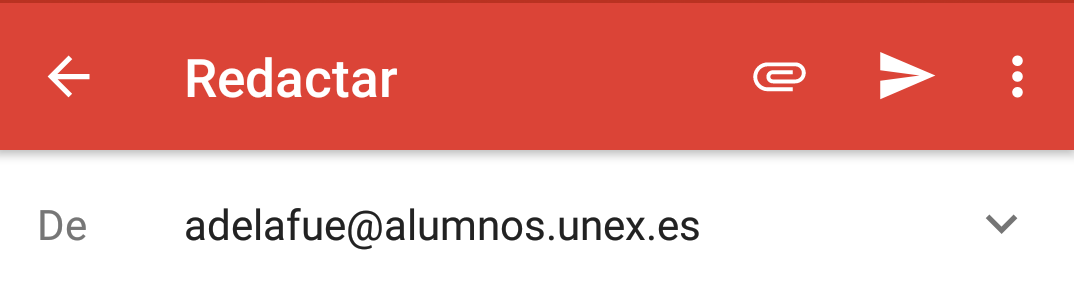
\includegraphics[scale=0.2]{pictures/IRL/GMail/nuevo_correo_gmail_emisor.png}
	    	\caption{Android Widget Spinner}{Elemento gráfico donde aparece el emisor.}
    		\label{fig:Android Widget Spinner}
		\end{center}
	\end{figure}

% -- new subitem
\item \textit{Widget MultiAutoCompleteTextView}. Elemento de la interfaz donde aparecen los receptores, la potencia del componente permite que con las primeras letras del correo del receptor se sugiera la dirección completa.
 	\begin{figure}[H]
		\begin{center}
     		
\includegraphics[scale=0.2]{pictures/IRL/GMail/nuevo_correo_gmail_receptor.png}
	    	\caption{Android Widget MultiAutoCompleteTextView}{Elemento gráfico donde aparece el receptor/es del correo.}
    		\label{fig:Android Widget MultiAutoCompleteTextView}
		\end{center}
	\end{figure}

% -- new subitem
\item \textit{Widget EditText}. Campo de texto donde escribir el asunto del correo. 
 	\begin{figure}[H]
		\begin{center}
     		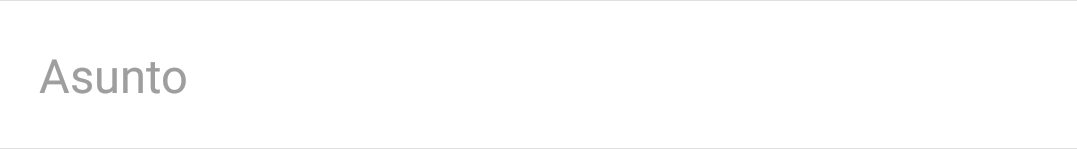
\includegraphics[scale=0.2]{pictures/IRL/GMail/nuevo_correo_gmail_asunto.png}
	    	\caption{Widget Edit Text}{Elemento de la interfaz donde escribir el asunto.}
    		\label{fig:Android Widget EditText}
		\end{center}
	\end{figure}


% -- new subitem 
\item \textit{View}. Vista editable a modo de caja de texto donde se redacta el cuerpo del correo. 
 	\begin{figure}[H]
		\begin{center}
     		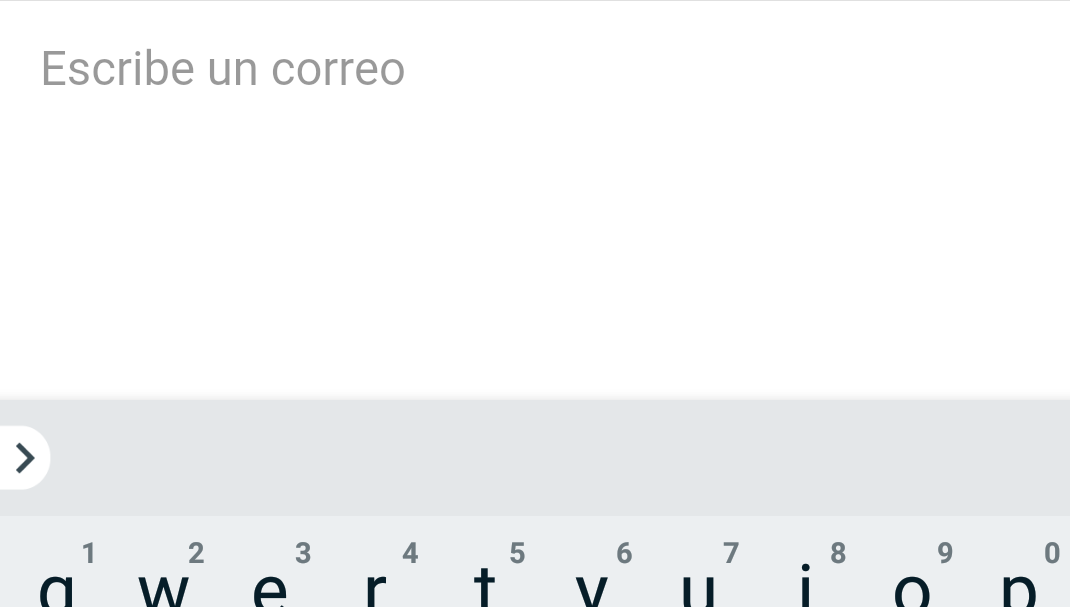
\includegraphics[scale=0.2]{pictures/IRL/GMail/nuevo_correo_gmail_cuerpo.png}
	    	\caption{Android View}{Elemento donde redactar el cuerpo.}
    		\label{fig:Android View}
		\end{center}
	\end{figure}
\end{itemize} % -- elementos de la interfaz
Cada uno de estos elementos descritos sobre la interfaz, generan un evento de accesibilidad que el analizador comprueba a través del nombre de la clase del elemento de la interfaz asociado al evento. Si el nombre coincide con alguno de los elementos aquí listados, se extrae el texto del evento y se infla en el GMailDto el atributo correspondiente (emisor, receptor, asunto y cuerpo). 
Por último, tenemos el elemento \textit{Widget Toast}, típico mensaje que aparece en la mitad inferior de la pantalla que informa de algún suceso. 
\newline
\newline
\begin{figure}[H]
		\begin{center}
     		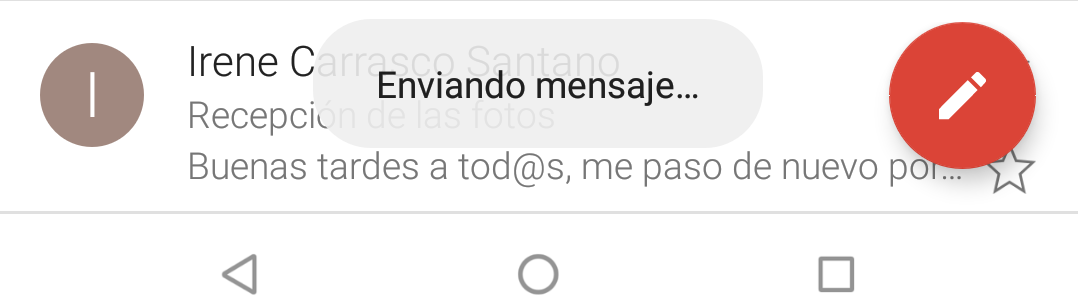
\includegraphics[scale=0.2]{pictures/IRL/GMail/correo_enviado.png}
	    	\caption{Android View}{Elemento donde redactar el cuerpo.}
    		\label{fig:Android View}
		\end{center}
	\end{figure}
En este caso el widget toast nos informa cada vez que se envía un correo, momento en el cual cerramos nuestro Dto y se lo pasamos al manejador de la base de datos para que lo persiste en la colección correspondiente. 
\item \textbf{DBManager}. Capa encargada de la persistencia, se encarga mapear los GMailDto a un modelo y almacenarlo en la base de datos local. 
\end{itemize} % -- niveles de app 
\section{Captura de Whatsapp}
Veamos ahora como es la captura de Whatsapp y cómo es la estructura del objeto en el que se asienta. 
\subsection{WhatsappDto}
Los atributos que componente este objeto son; 
\begin{verbatim}
public class WhatsappDto extends RealmObject {
	@PrimaryKey
    private String id;

    /** Name of the contact who the user is talking to*/
    private String interlocutor;

    /** A list of the messages sent, including the timestamp of the send */
    private RealmList<TimestampString> textList;

    /** Describes the timestamp when the user clicked a conversation */
    private Date startTimestamp;

    /** Describes the timestamp when the user abandoned a conversation */
    private Date endTimestamp;
    
    // -- getters and setters
}
\end{verbatim}
En primer lugar, el consabido identificador, necesario para la base de datos. 
\newline \newline 
A este identificado le sigue el atributo \textbf{interlocutor}, destinado a almacenar el nombre del contacto con quien el usuario está hablando. 
\newline \newline 
A continuación figura una RealmList con objetos del tipo TimestampString. 
\begin{verbatim}
public class TimestampString extends RealmObject {

    /** String with the content of the text */
    private String text;

    /** Timestamp describing the exact moment when the text was written */
    private Date timestamp;
   
   // -- getters and setters 
}
\end{verbatim}
Este tipo de objeto consiste en un String, para almacenar la cadena enviada, y un timestamp para controlar el momento exacto del envío de la misma. 

Por último, en WhatsappDto, nos encontramos con dos java.util.Date, \textbf{startTimestamp}, para almacenar el momento en el que el usuario abre una conversación, y en \textbf{endTimestamp} para, como sospecharán los lectores más hábiles, almacenar el momento exacto en el que esa misma conversación es abandonada. 
\subsection{Diagrama de actividad}
En la captura de los mensajes enviados con Whatsapp entran en juego dos tipos de eventos. Por un lado, aquellos que pertenecen (ó cuyo nombre del paquete) corresponde con el propio Whatsapp, \textit{com.whatsapp}, y por el otro, los relacionados con el teclado, \textit{com.google.android.inputmethod.latin}.
\newline \newline 
Jugando con estos dos eventos seremos capaces de recoger con quién habla el usuario, lo que escribe y durante cuanto tiempo permanece en una conversación o en la propia pantalla principal de la aplicación. Veámoslo por partes. 
\subsubsection{Eventos de com.whatsapp} 
Este tipo de evento, cuyo origen es la propia aplicación de Whatsapp, nos aportará información acerca de los gestos que realiza el usuario dentro de la misma. Gracias a esto, podremos añadir un contexto a la información recogida, puesto que nos permiten obtener datos como el nombre del contacto con el que habla el usuario, a la vez que nos aportan información acerca de la pantalla que está viendo el usuario a cada momento.
\newline \newline
A la hora de recoger el texto vertido por el usuario en una conversación determinada la captura se complica, puesto que entran en juego eventos externos, sin los cuales no podríamos dotar de sentido a las cadenas escritas. Veámoslo en detalle, dado que no es un asunto trivial. Expliquemos en primer lugar cómo se capturan los caracteres escritos. 
\newline \newline 
Cuando escribimos un mensaje en el campo de texto de la aplicación, se generan tantos eventos de accesibilidad como letras pulsadas en el teclado. Estos eventos son originados por Whatsapp, con lo cual seguirán el flujo destinado para su captura, y diferenciando el widget de la UI asociado al mismo, podremos capturar el texto del evento, donde se encuentra nuestra preciada información, las letras que el usuario pulsa. 
\newline \newline
Pero al mismo tiempo, contamos con un inconveniente, y es que esta generación de contenido es \textit{dummy}, es decir, únicamente recibimos información a chorro, sin saber cuando se envía una cadena, cuando se borra o cuando un mensaje es descartado navegando hacia atrás en la pantalla. 
\newline \newline 
Para darle sentido a este flujo continuo de información deberemos atender los eventos que genera el teclado. 
\subsubsection{Eventos de com.google.android.inputmethod.latin}
Estos eventos nos aportan la información de lo que hace el usuario con el teclado a través del texto que muestra a modo de \textit{placeholder}. De esta forma, cuando el teclado se muestra por primera vez o el campo está vacío, el texto asociado al evento generado será \textit{Mostrando teclado español (España) (QWERTY (Ñ))} (en el caso de usar un teclado con la distribución en español). 
\newline \newline 
Pero no es tan sencillo como aparentemente parece, puesto el teclado genera eventos de este tipo cada vez que el usuario hace gestos inesperados, como por ejemplo mandar un emoji, buscar un gif o simplemente cambiar al teclado de símbolos para acceder a los números o símbolos de puntuación. 
\newline \newline 
Manteniendo esto en mente, podemos saber cuándo el usuario acaba de enviar una cadena de texto, dado que cada vez que el campo de texto se queda vacío (recordemos el funcionamiento de la app, cuando enviamos un mensaje se vacía el campo), significa que el usuario ha mandado una cadena. Cada vez que un evento con estas características es generado, se notificará al analizador de WhatsApp mediante la llamada al método \textit{confirmKeyboardInput}, el cual verificará el estado del Dto que contiene la información capturada hasta el momento. 
\newline \newline 
Esta verificación del estado del objeto consiste en chequear la correcta inicialización de las variables, que no se ha capturado una cadena vacía ó que el texto capturado no se corresponde con el \textit{placeholder} que incrusta Whatsapp en su aplicación, que reza \textit{Escribir mensaje}. 
\newline \newline
Una vez pasado este primer chequeo, se comprueba el array donde almacenamos las cadenas escritas junto a su timestamp. Dado que los eventos, dependiendo de los gestos del usuario, pueden venir duplicados, (por ejemplo cambiar el layout del teléfono, abrir y cerrar el teclado, etc), deberemos comprobar que, en caso de que el array no esté vacío, la cadena a añadir no exista en el array. 
\newline \newline 
La captura del resto de campos (interlocutor y pantalla principal) es sencilla, como hemos dicho, para esto sólo atenderemos a los eventos generados por Whatsapp. Una vez establecido este primer filtro, deberemos tratar los eventos en función del elemento de la interfaz asociado al mismo, ó dicho en términos de implementación, el \textit{className} del origen del evento. De esta forma tenemos: 
\begin{itemize}
\item \textit{com.whatsapp.HomeActivity}. Se corresponde a la pantalla principal del Whatsapp. Nos sirve para almacenar en la base de datos cualquier objeto existente que contenga información. Una vez hecho esto, instanciamos una nueva versión del mismo y limpiamos los atributos de la clase relacionados con el interlocutor y el mensaje que escribe el usuario. 
\begin{figure}[H]
	\begin{center}
     	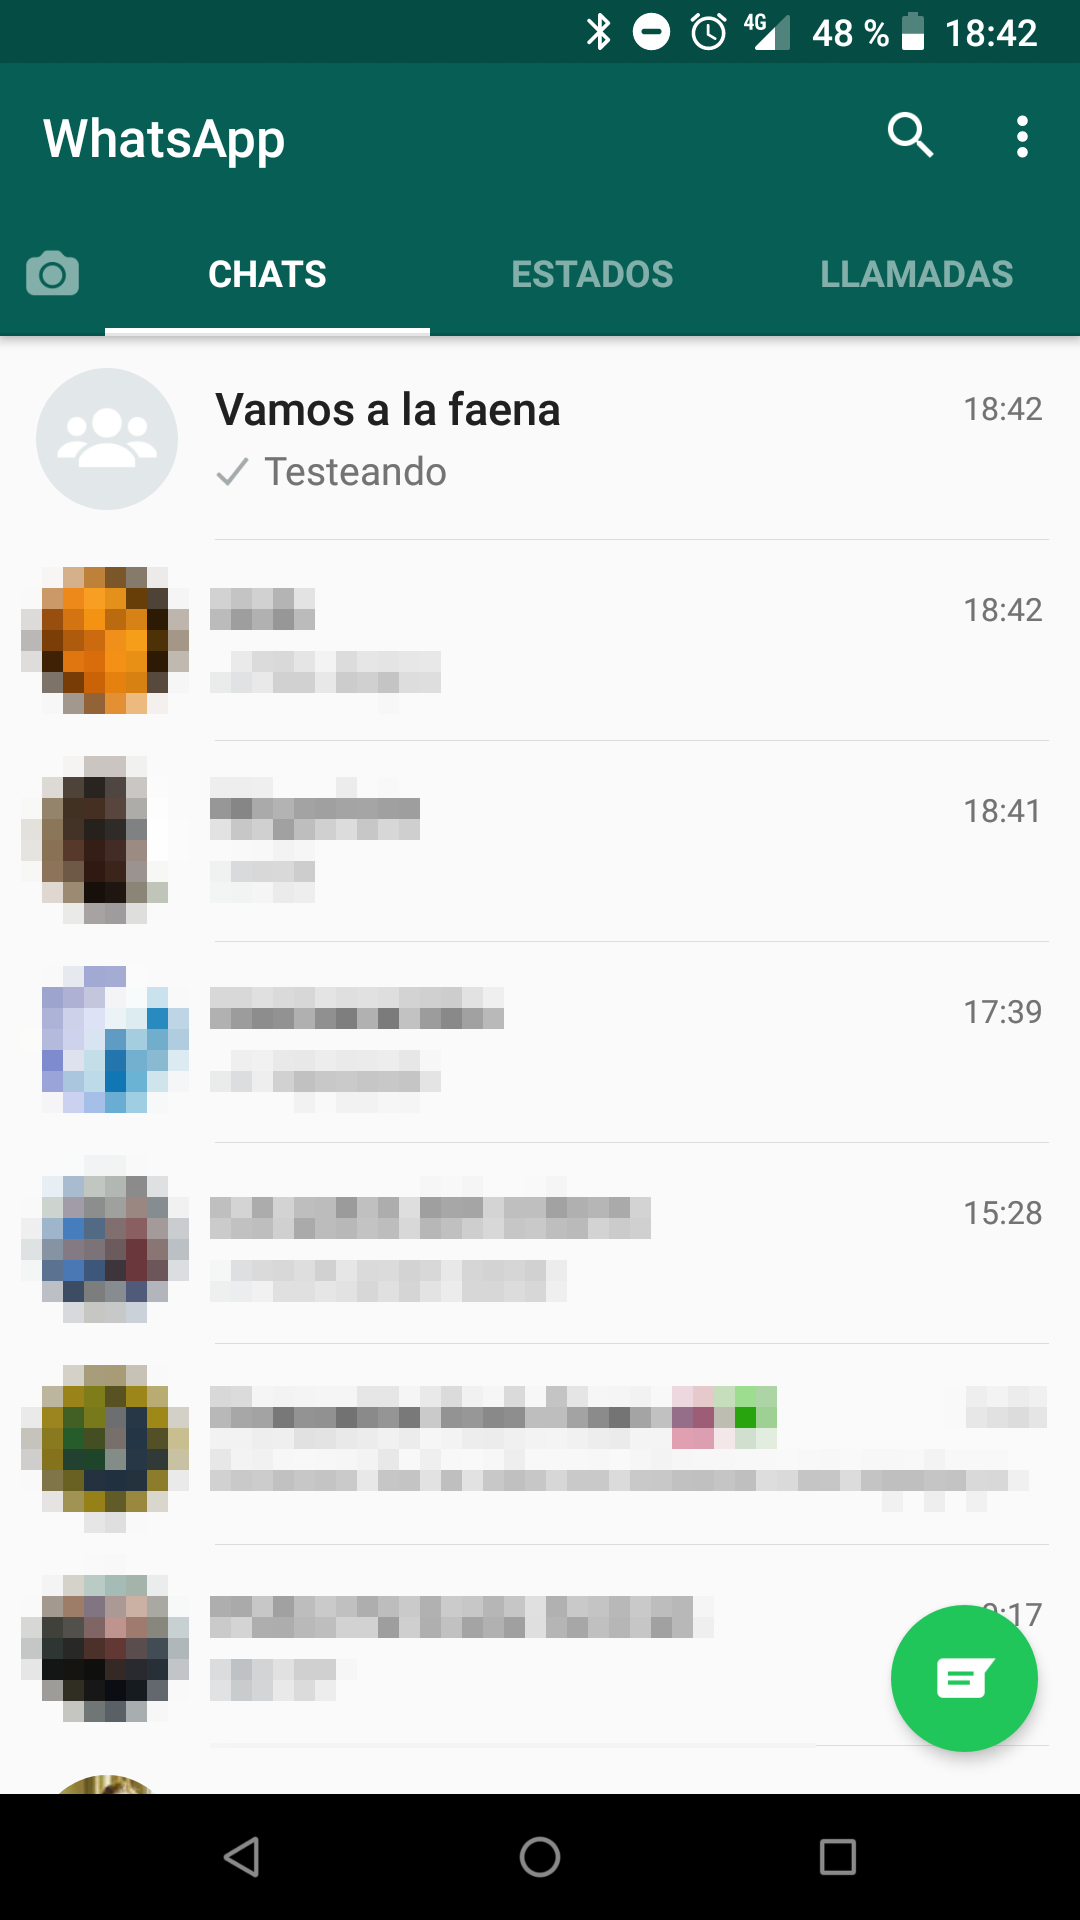
\includegraphics[scale=0.15]{pictures/IRL/whatsapp/whatsapp_home.png}
	    	\caption{Whatsapp Home}{Pantalla principal de Whatsapp}
    	\label{fig:Whatsapp Home}
	\end{center}
\end{figure}

\item \textit{android.widget.RelativeLayout}. Por si sólo, un relative layout es simplemente una patrón para disponer los elementos en la pantalla, pero si su origen es Whatsapp (recordemos, el nombre del paquete, un filtro que en este momento ya se ha superado), sabremos que el usuario ha pulsado sobre una conversación. 
\newline \newline 
Además, el mismo evento que nos indica la entrada en una conversación lleva asociado el nombre del contacto, con lo cual para saber con quién está hablando el usuario bastará con extraer el texto del evento. 
\begin{figure}[H]
	\begin{center}
     	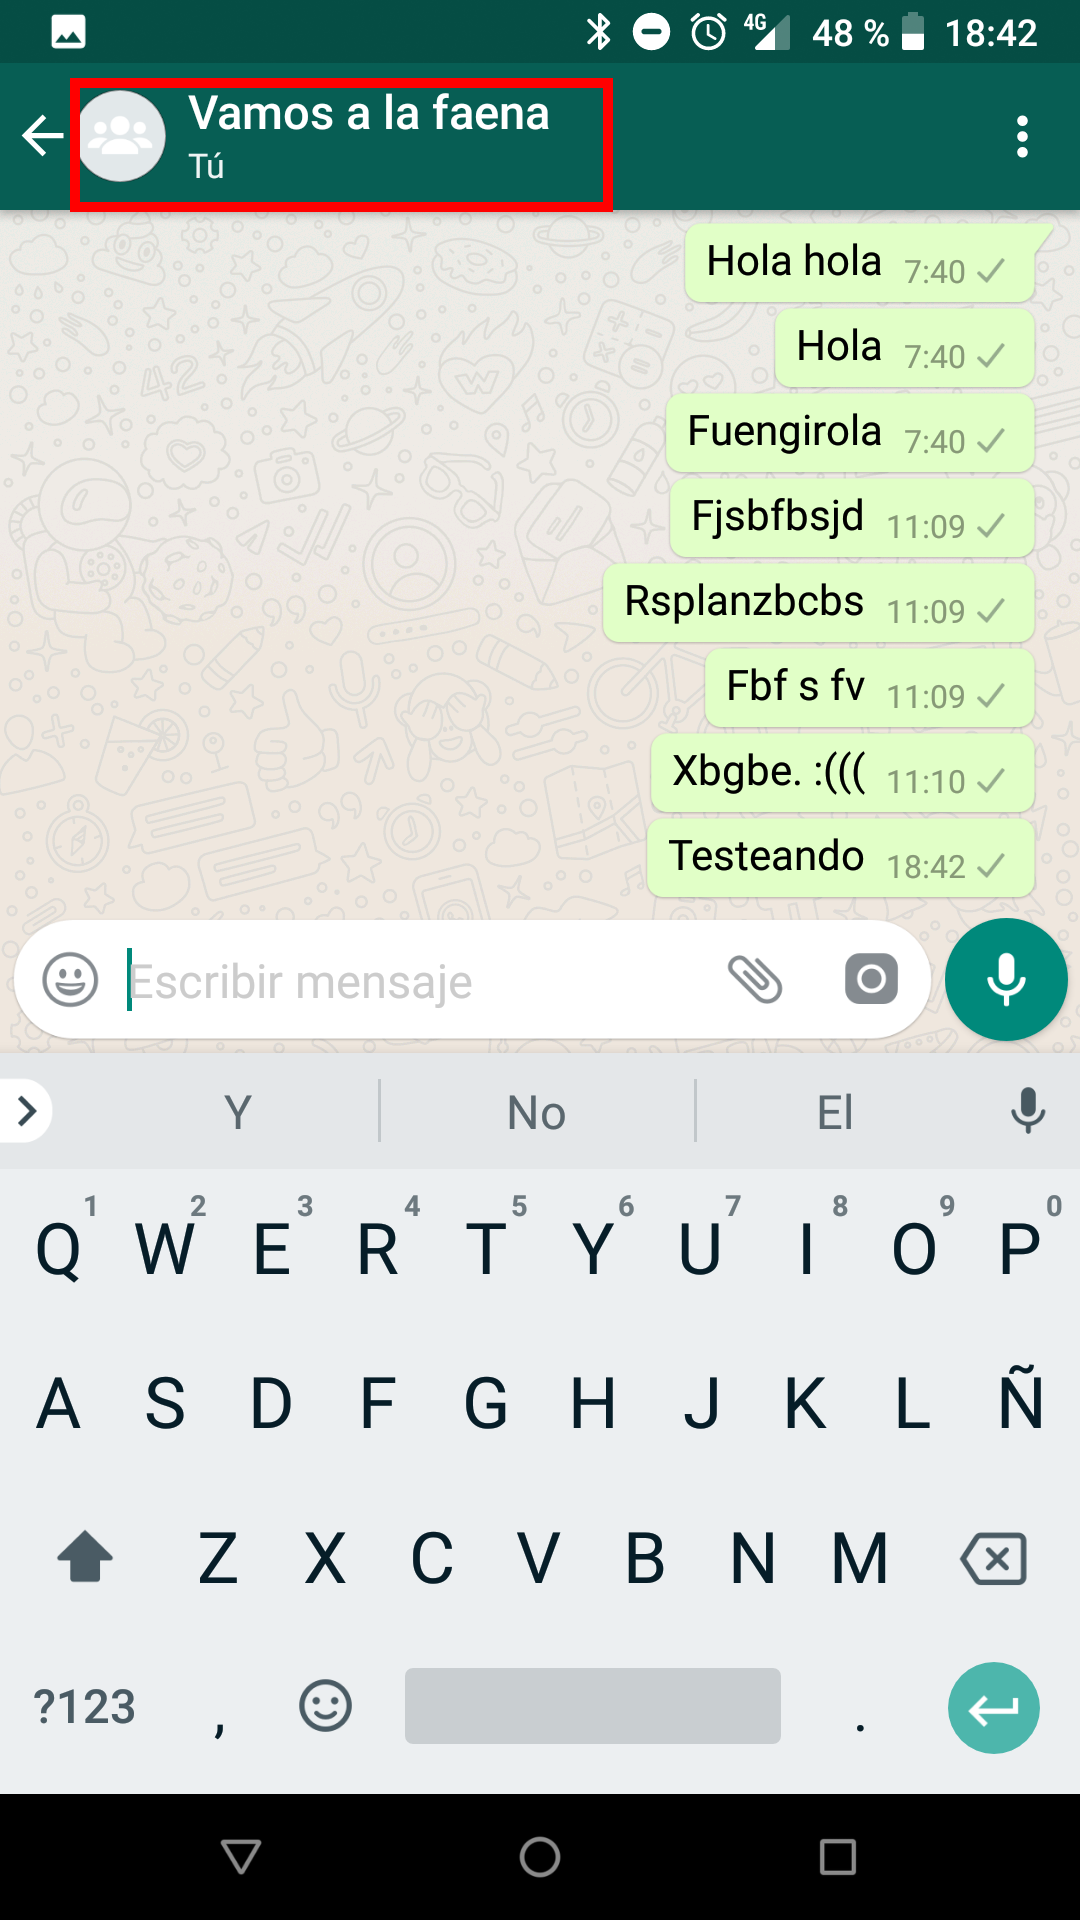
\includegraphics[scale=0.15]{pictures/IRL/whatsapp/whatsapp_layout.png}
	    	\caption{Whatsapp layout de una conversación}{Layout de una conversación de usuario}
    	\label{fig:Whatsapp Relative Layout}
	\end{center}
\end{figure}
\item \textit{android.widget.EditText}. Como es obvio, este evento estará asociado al campo de texto donde el usuario escribe su conversación. Deberemos, por tanto, capturar en todo momento el texto que llevan asociados este tipo de eventos, puesto que ahí estará el contenido real de lo que el usuario está escribiendo a su contacto. 
\newline \newline 
Este contenido se irá almacenando en una variable que se añadirá al Dto asociado cuando entre en juego un evento de teclado. Con las condiciones descritas anteriormente, recordemos, eventos con nombre de paquete \textit{com.google.android.inputmethod.latin} y cuyo texto implique la acción de mostrar el teclado limpio, esperando una nueva entrada de texto. 
\begin{figure}[H]
	\begin{center}
     	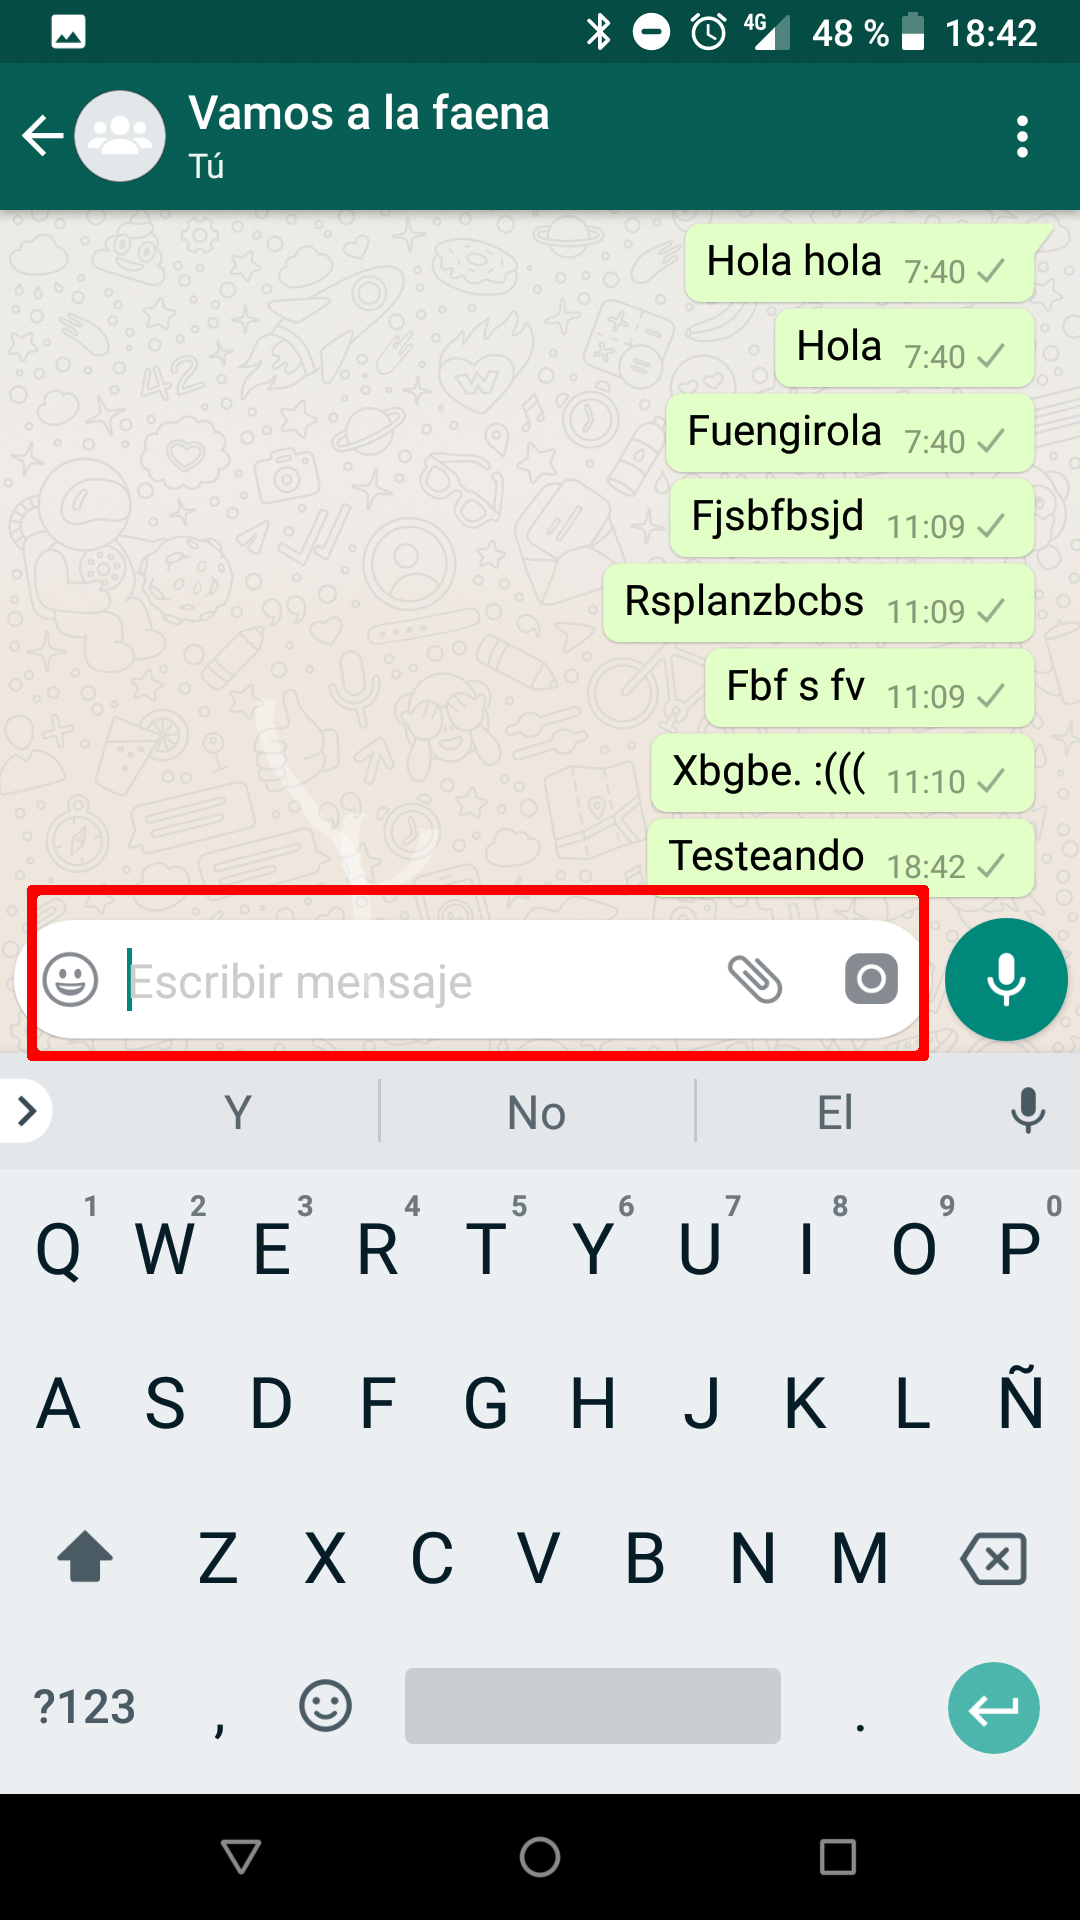
\includegraphics[scale=0.15]{pictures/IRL/whatsapp/whatsapp_text.png}
	    	\caption{Campo de texto de Whatsapp}{Campo de texto de Whatsapp}
    	\label{fig:Whatsapp editText widget}
	\end{center}
\end{figure}
\end{itemize}
Veamos ahora, mediante un diagrama de actividad, una visualización gráfica del algoritmo de captura descrito anteriormente. 
\begin{landscape}
\begin{figure}[htb]
	\begin{center}
     	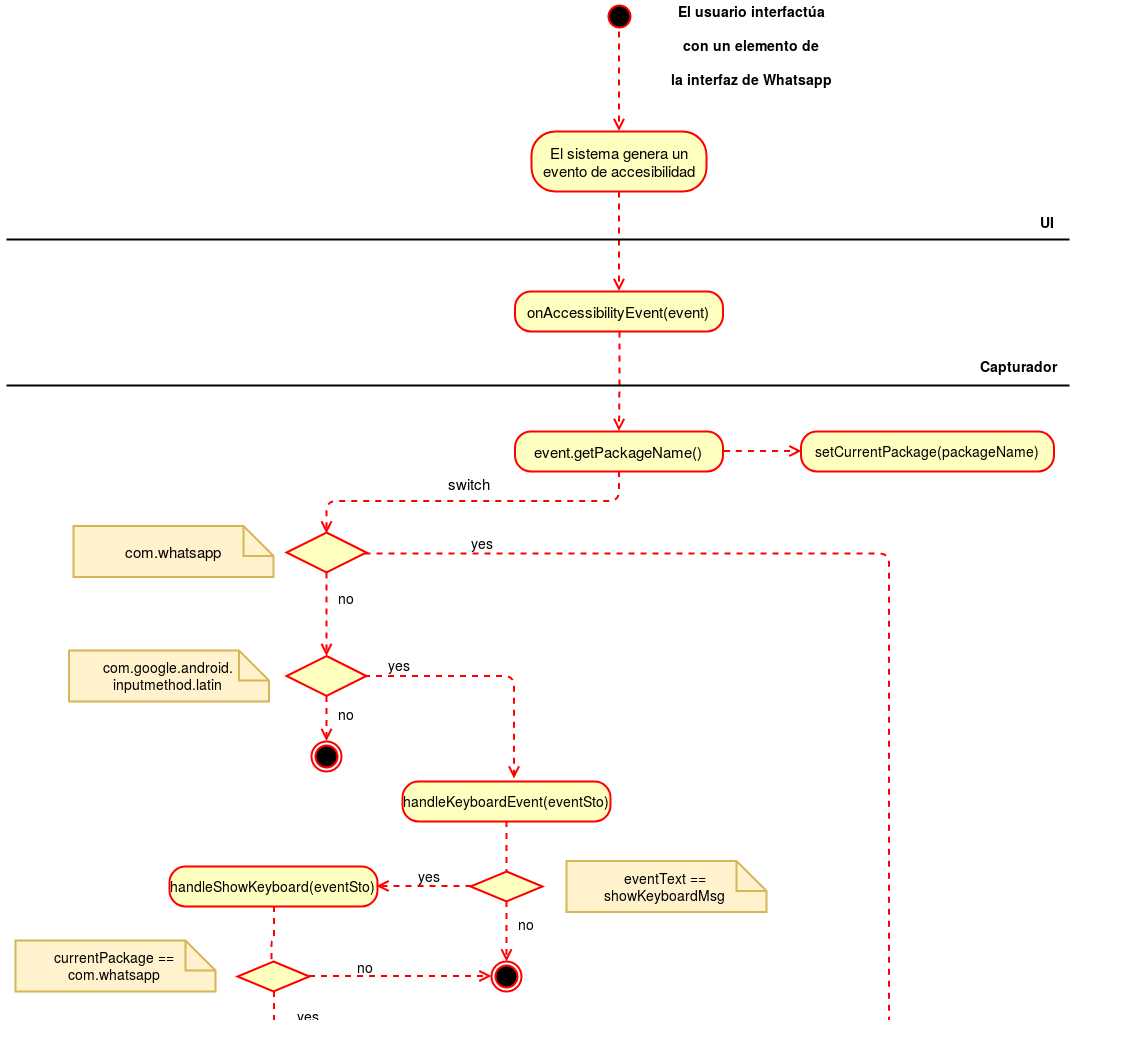
\includegraphics[scale=0.4]{pictures/activity/whatsappActivityDiagram1.png}
	    	\caption{Diagrama de actividad de Whatsapp (1)}{Diagrama de actividad de Whatsapp (1)}
    	\label{fig:Diagrama de actividad Whatsapp (1)}
	\end{center}
\end{figure}
\end{landscape}
\begin{landscape}
\begin{figure}[htb]
	\begin{center}
     	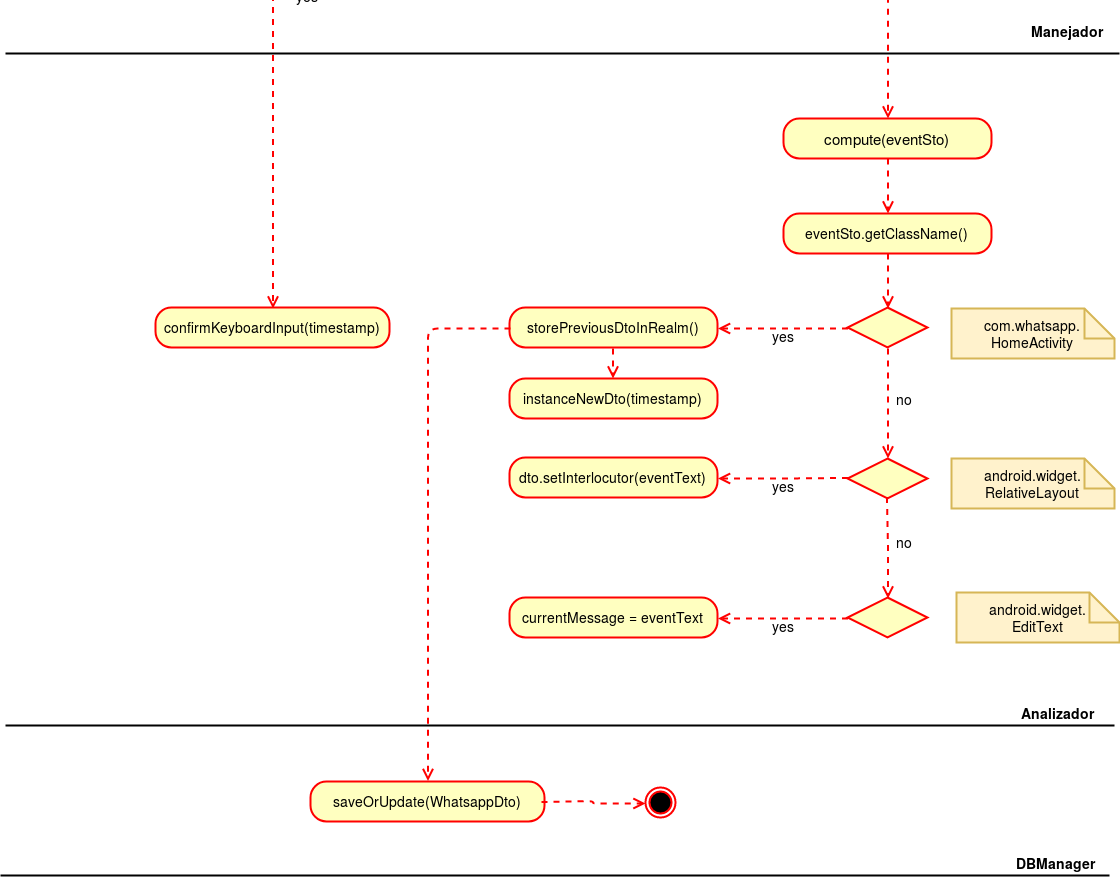
\includegraphics[scale=0.4]{pictures/activity/whatsappActivityDiagram2.png}
	    	\caption{Diagrama de actividad de Whatsapp (2)}{Diagrama de actividad de Whatsapp (2)}
    	\label{fig:Diagrama de actividad Whatsapp (2)}
	\end{center}
\end{figure}
\end{landscape}
Como vemos, el algoritmo de captura recae en su mayor parte en el WhatsappAnalyzerImpl. Vemos sendas actividades vinculadas a métodos. Analicemos en que consisten estos métodos, puesto que conforman los pilares sobre los que se asientan la caputura. 
\subsubsection{Compute(eventSto}
Este método recibe una instancia de la clase EventSto, que como ya hemos visto, incluye el propio evento de accesibilidad, su className y packageName. 
\newline \newline 
Mirando el className construimos un switch, que en función de su valor dirige el flujo de captura hacia un lado u otro. 
\newline \newline
En caso de coincidir el valor con \textit{com.whatsapp.HomeActivity}, llamaremos al método que chequea y guarda en la base de datos cualquier instancia existente del WhatsappDto. 
\newline \newline 
Si por el contrario nos encontramos con \textit{android.widget.RelativeLayout}, sabremos que el usuario ha entrado en una conversación de Whatsapp, deberemos por tanto setear el valor del interlocutor al correspondiente al texto extraído del evento. 
\newline \newline 
Por último, si estamos tratando con un evento relacionado con \textit{android.widget.EditText}, significará que el usuario se encuentra escribiendo en el campo de texto, y deberemos extraer y almacenar el propio texto del evento. 
\subsubsection{storeObjectInRealm()}
Es el método responsable de llamar al DBManager para persistir el objeto en el que estamos guardando la información de captura de una conversación. 
\newline \newline 
En primer lugar, este método asigna el timestamp del momento de captura del evento al atributo endTimestamp del WhatsappDto, de esta forma añadiremos al contexto del usuario el momento exacto en el que abandona la conversación con su contacto. 
\newline \newline 
Una vez hecho esto, se realiza una comprobación del resto de atributos del dto, incluyendo, que exista el propio objeto (que no sea nulo) y que el interlocutor no sea una cadena vacía. Si estas condicione se cumplen, el objeto será almacenado en la base de datos del teléfono llamando al DBManager. 
\subsubsection{instanceNewDto(timestamp)}
El nombre del método clarifica bastante su tarea. Esta consiste en instanciar un nuevo objeto del tipo WhatsappDto y añadirle el timestamp, cuyo origen es el momento en que se capturó el evento, para asignarlo al atributo startTimestamp del nuevo objeto WhatsappDto. 
\newline \newline 
De esta manera aportamos contexto a la captura, puesto que nos permite conocer el momento exacto en el que un usuario abre una conversación. Esto, junto con el endTimestamp nos permitirá averiguar cuánto tiempo pasa el usuario en cada una de sus conversaciones. 
\subsubsection{confirmKeyboardInput(timestamp)}
A este método público se le llama directamente desde el manejador de eventos. Esto ocurre cuando se detecta un evento de teclado que coincide con la apertura del teclado ó sencillamente cuando el teclado se vacía después de escribir. 
\newline \newline 
Como se ha explicado al inicio de esta sección, esto se traduce en el hecho de que el usuario ha mandado la cadena que se encontraba escribiendo, por lo tanto el método debe encargarse de chequear la validez de esa cadena y añadirla a la lista de mensajes del WhatsappDto
\newline \newline 
Gracias a este algoritmo, conseguiremos una completa recolección de lo que hace el usuario dentro del Whatsapp, sabremos con quien habla, lo que dice y durante cuanto tiempo se relaciona con sus contactos. Esta información por lo tanto se denota muy valiosa, ya que Whatsapp es la aplicación más usada para hablar con nuestro alegados, gracias al contexto aportado podremos conocer de que forma se relaciona el usuario con su entorno social más cercano. 
\section{Captura de Chrome}
La captura de las búsquedas y páginas realizadas Chrome se antoja más sencilla, puesto que sólo necesitamos controlar las cadenas de búsqueda así como la marca horaria en la que fueron realizadas. 
\subsection{ChromeDto}
El objeto sobre el que construimos la información capturada durante la navegación tiene el siguiente aspecto; 
\begin{verbatim}
public class ChromeDto extends RealmObject {

    @PrimaryKey
    private String id;

    /** String containing the visited urls or search terms */ 
    private String searchUrl;

    /** Timestamp when the search happened */ 
    private Date timestamp;
	
	// -- getters and setters 
}
\end{verbatim}
Obviemos ahora el id de Realm. Tenemos por un lado el atributo \textbf{searchUrl}, destinado a almacenar la url de las páginas visitadas o los términos de una búsqueda. 
\newline \newline 
Por otro, el atributo \textbf{timestamp}, de tipo java.util.Date, que nos ayudará a situar en un marco temporal las búsquedas del usuario. De este modo persiguiendo nuestro objetivo de lograr un perfil lo más completo del mismo, podremos saber en qué momento del día el usuario realiza sus búsquedas Web, conociendo además el motivo de esa búsqueda. 
\subsection{Diagram de actividad}
De nuevo, nos encontramos en una situación en la que necesitamos controlar dos tipos de evento, por un lado los relacionados con la propia aplicación de Chrome, \textit{com.android.chrome}, y por otro, el teclado \textit{com.google.android.inputmethod.latin}. 
\subsubsection{Eventos de com.android.chrome}
Estos eventos nos permitirán conocer lo que el usuario escribe en la barra de búsqueda, así como los sitios frecuentes que la propia aplicación muestra cada vez que abrimos una nueva pestaña. 
\newline 
\newline 
Veamos a que elemento de la interfaz están relacionados los eventos para estos dos flujos de información; 
\begin{itemize}
\item \textit{android.widget.EditText}. Generado cuando el usuario escribe en la barra de búsuqeda. Por lo tanto, y del mismo modo que ocurría en Whatsapp, deberemos ir almacenando en una variable los caracteres vertidos por el usuario en esa barra de búsqueda. Ya llegará la confirmación por parte de un evento de teclado, que veremos mas adelante, para persistir esa información. 
\begin{figure}[H]
	\begin{center}
     	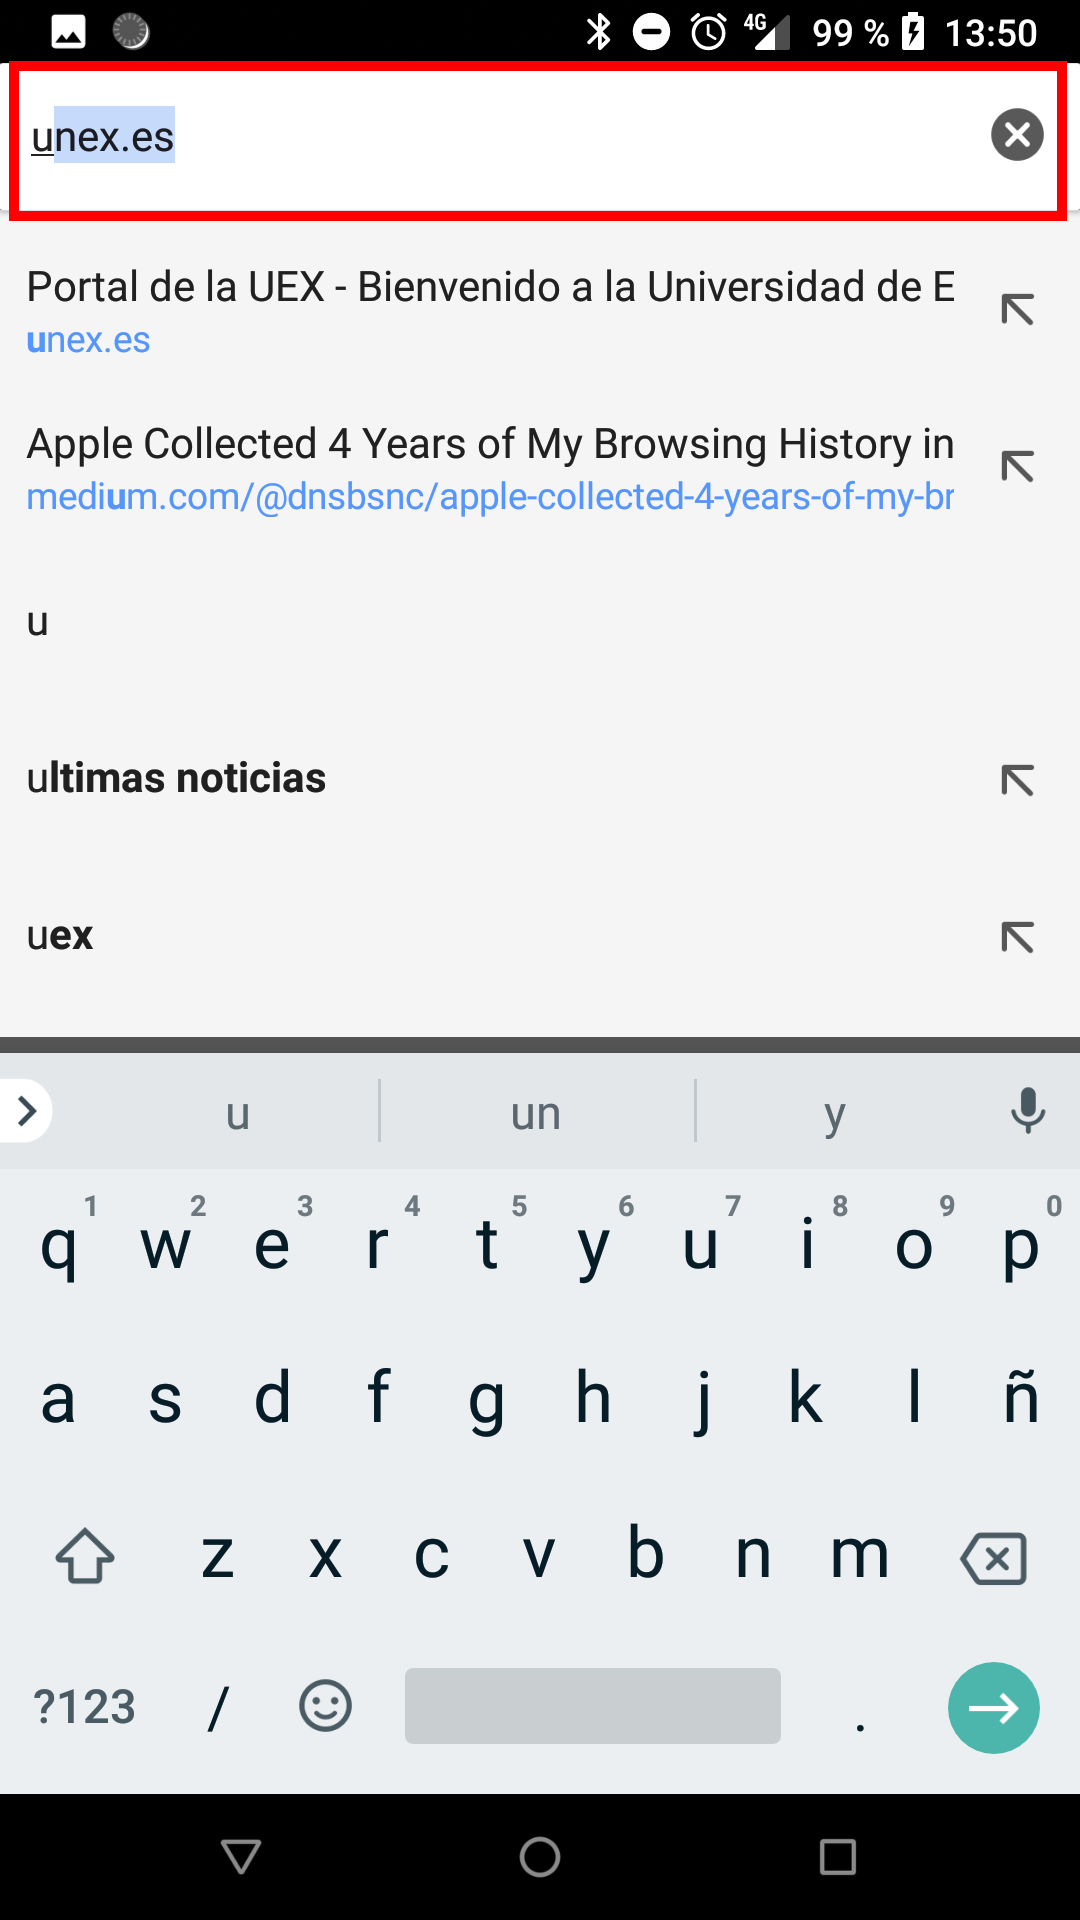
\includegraphics[scale=0.15]{pictures/IRL/chrome/chrome_editText.png}
	    	\caption{Componente edit text de Chrome)}{Componente edit text de Chrome}
    	\label{fig:Componente edit text de Chrome}
	\end{center}
\end{figure}
\item \textit{android.widget.FrameLayout}. Asociados a la pulsación de una página guardada como sitios frecuentes. Dado que el usuario, este caso, no tiene que escribir nada en la barra de búsqueda, deberemos obtener la página visitada obteniendo el texto de este evento. De esta forma podremos saber que sitios visita en cada ocasión, y,	 además, almacenar su dirección. 
\begin{figure}[H]
	\begin{center}
     	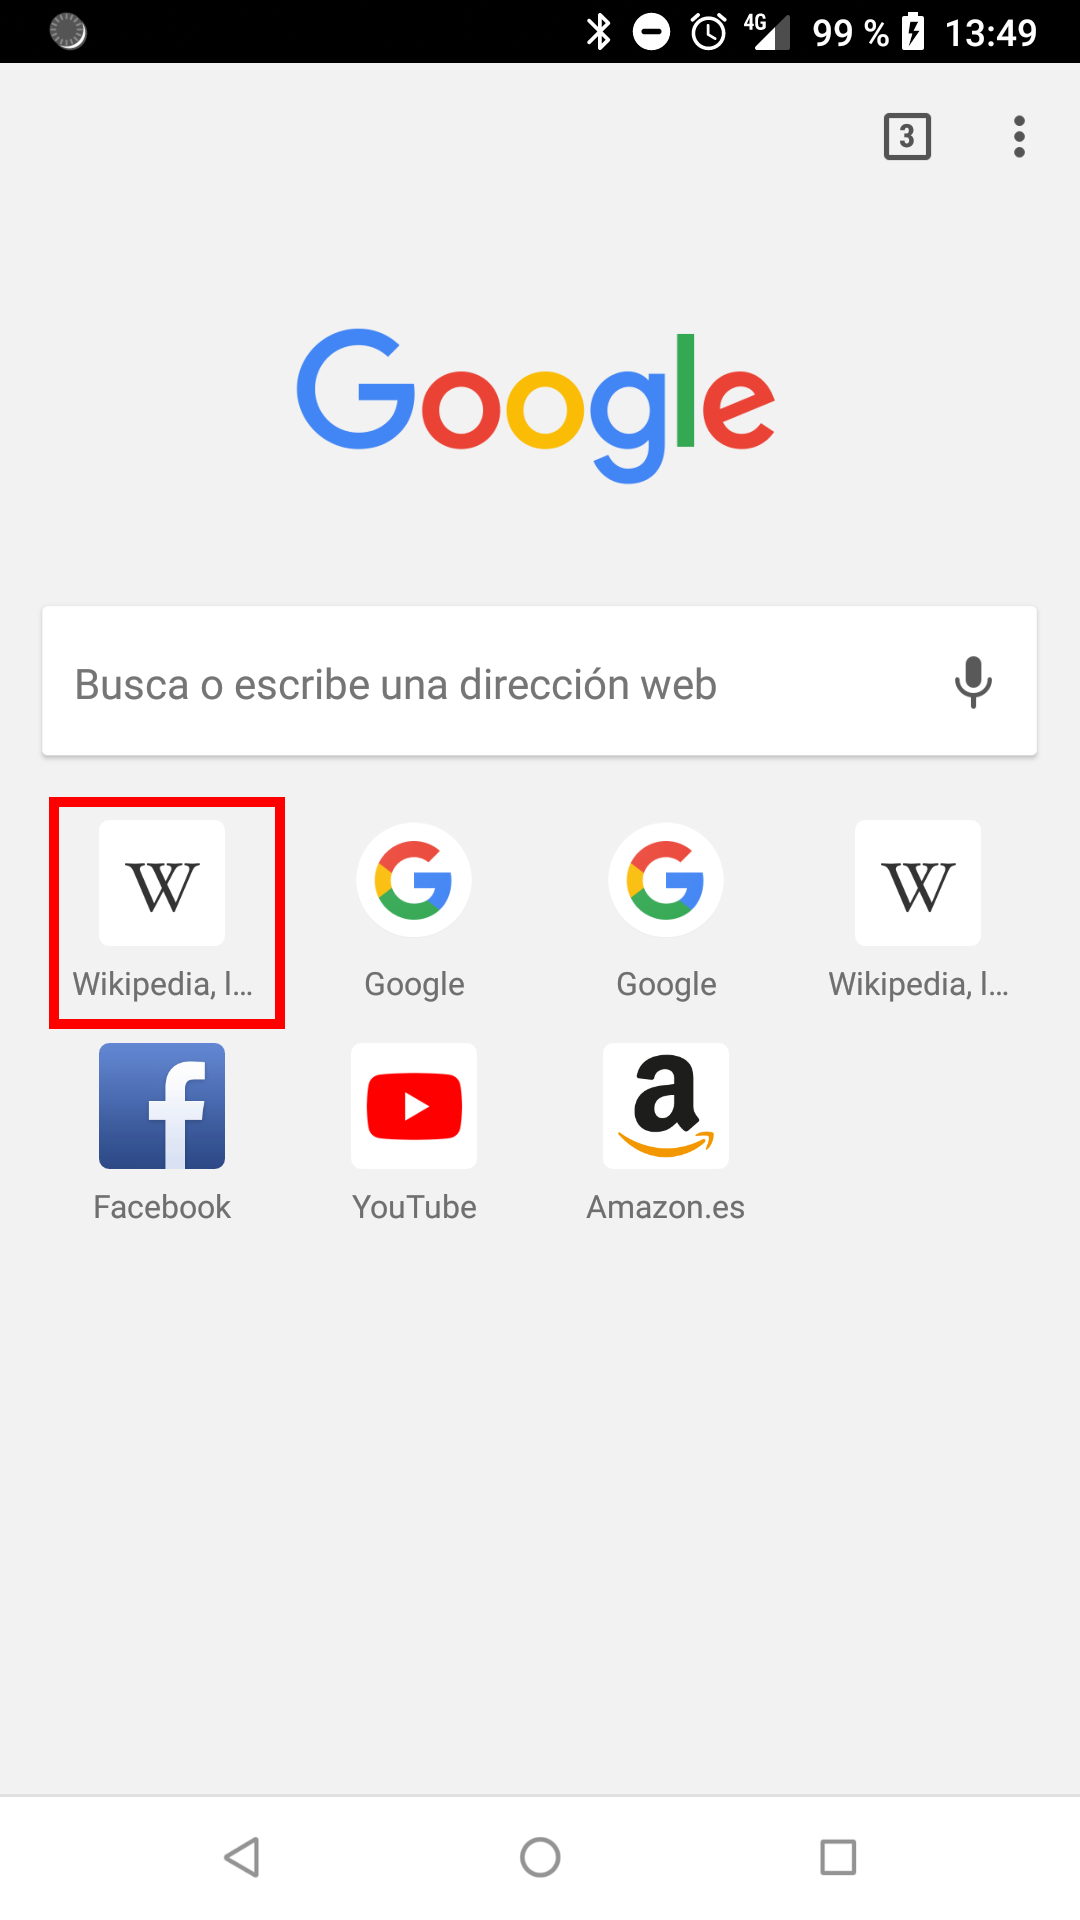
\includegraphics[scale=0.15]{pictures/IRL/chrome/chrome_frequents.png}
	    	\caption{Componente frameLayout de sitios frecuentes en Chrome)}{Componente frameLayout de sitios frecuentes en Chrome}
    	\label{fig:Componente frame layout de Chrome}
	\end{center}
\end{figure}
\item \textit{android.view.ViewGroup}. Se ejecutan cuando el usuario pulsa sobre alguna de las sugerencias que va generando la aplicación a medida que el usuario escribe la url o búsqueda. Este flujo debe estar incluido, porque cuando el usuario acepta alguna de estas sugerencias no se generan, como es obvio, eventos asociados a la escritura, si no que siguen su propio camino. Capturando estos eventos nos aseguramos de que nada se escapa en nuestra recolección de información. 
\begin{figure}[H]
	\begin{center}
     	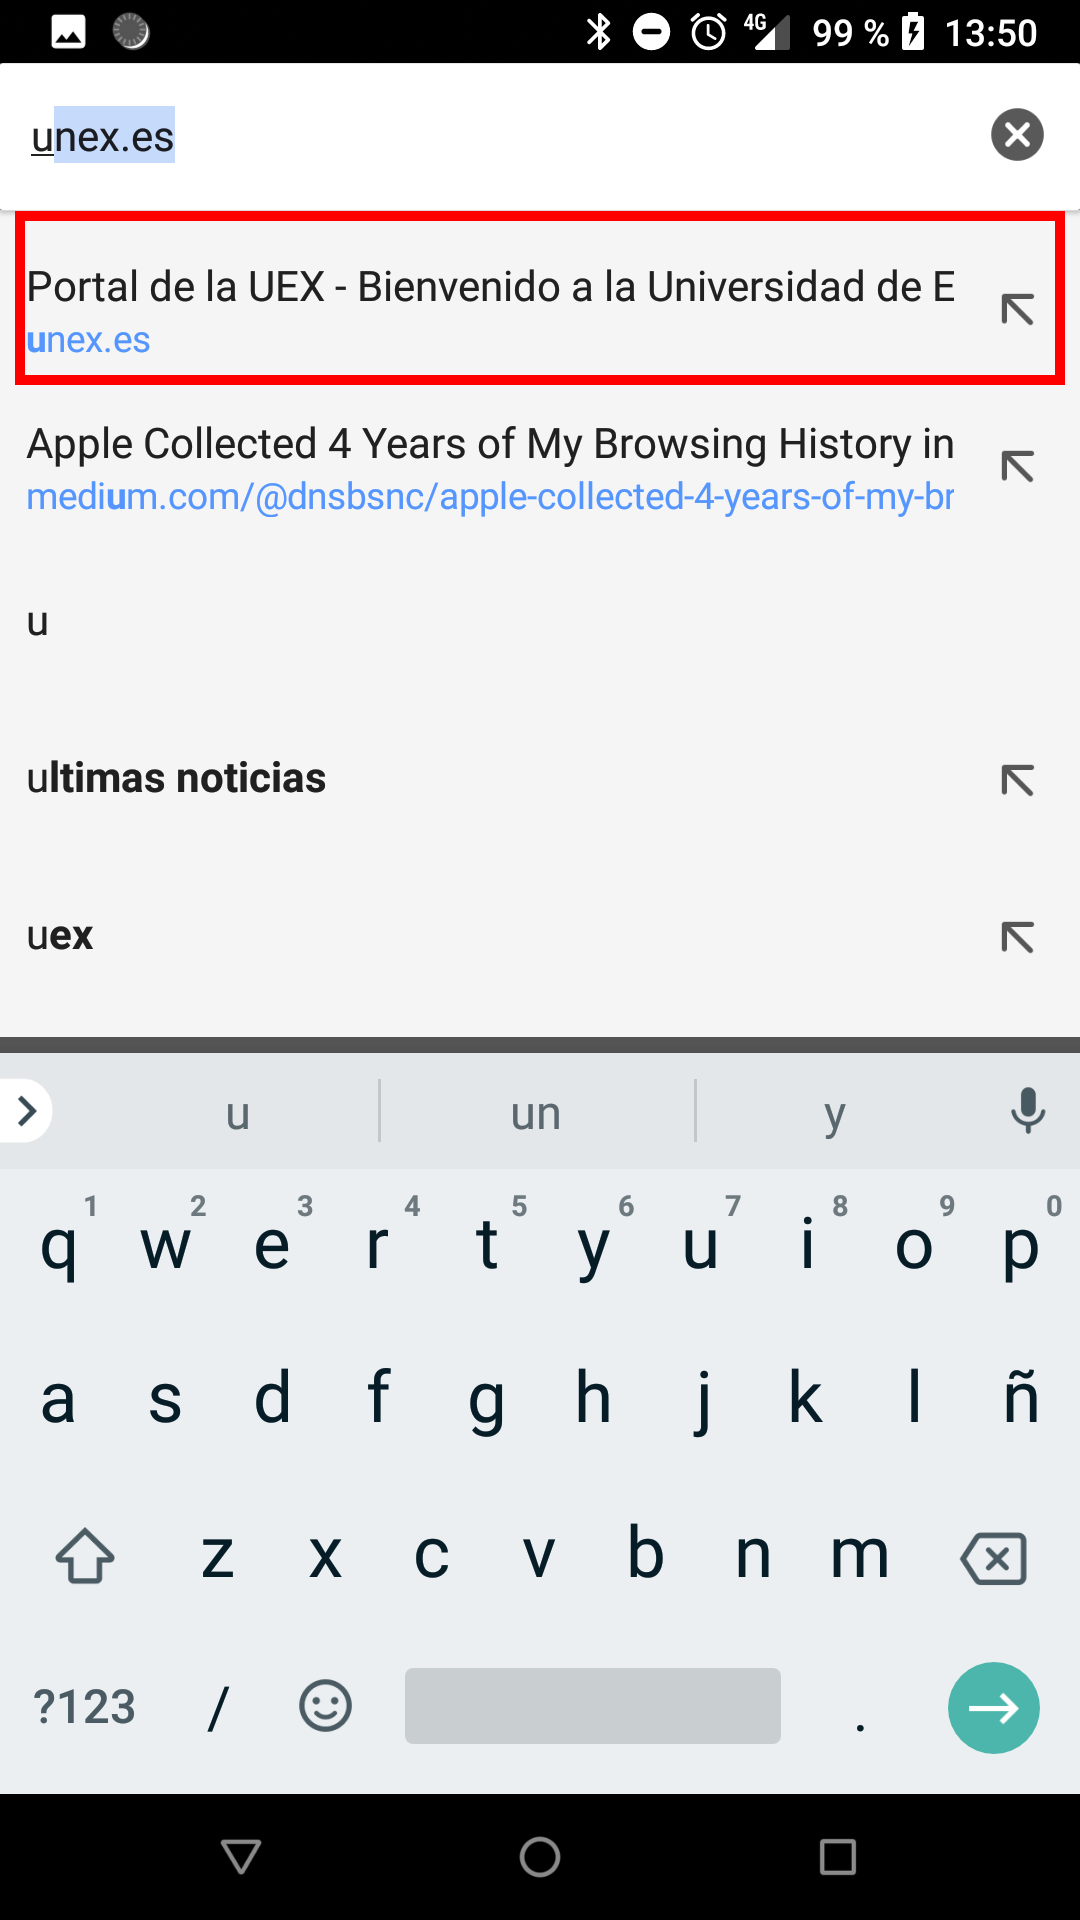
\includegraphics[scale=0.15]{pictures/IRL/chrome/chrome_view.png}
	    	\caption{Componente view group de sugerencias en Chrome)}{Componente view de sugerencias en Chrome}
    	\label{fig:Componente view group de Chrome}
	\end{center}
\end{figure}
\end{itemize}
\subsubsection{Eventos de com.google.android.inputmethod.latin}
Usaremos los eventos del teclado en su otra vertiente, puesto que nos interesa ahora saber cuando el teclado se oculta. 
\newline \newline 
Si recordamos como funciona esta app, cada vez que realizamos una búsqueda, el teclado se oculta para poder mostrar la página completa. Esto para nosotros es muy útil, puesto que cada vez que esto ocurre, significa que el usuario ha realizado una búsqueda. 
\newline \newline
Veamos ahora, mediante un diagrama de actividad, cómo es el flujo que sigue este proceso de captura. 
\begin{landscape}
\begin{figure}[htb]
	\begin{center}
     	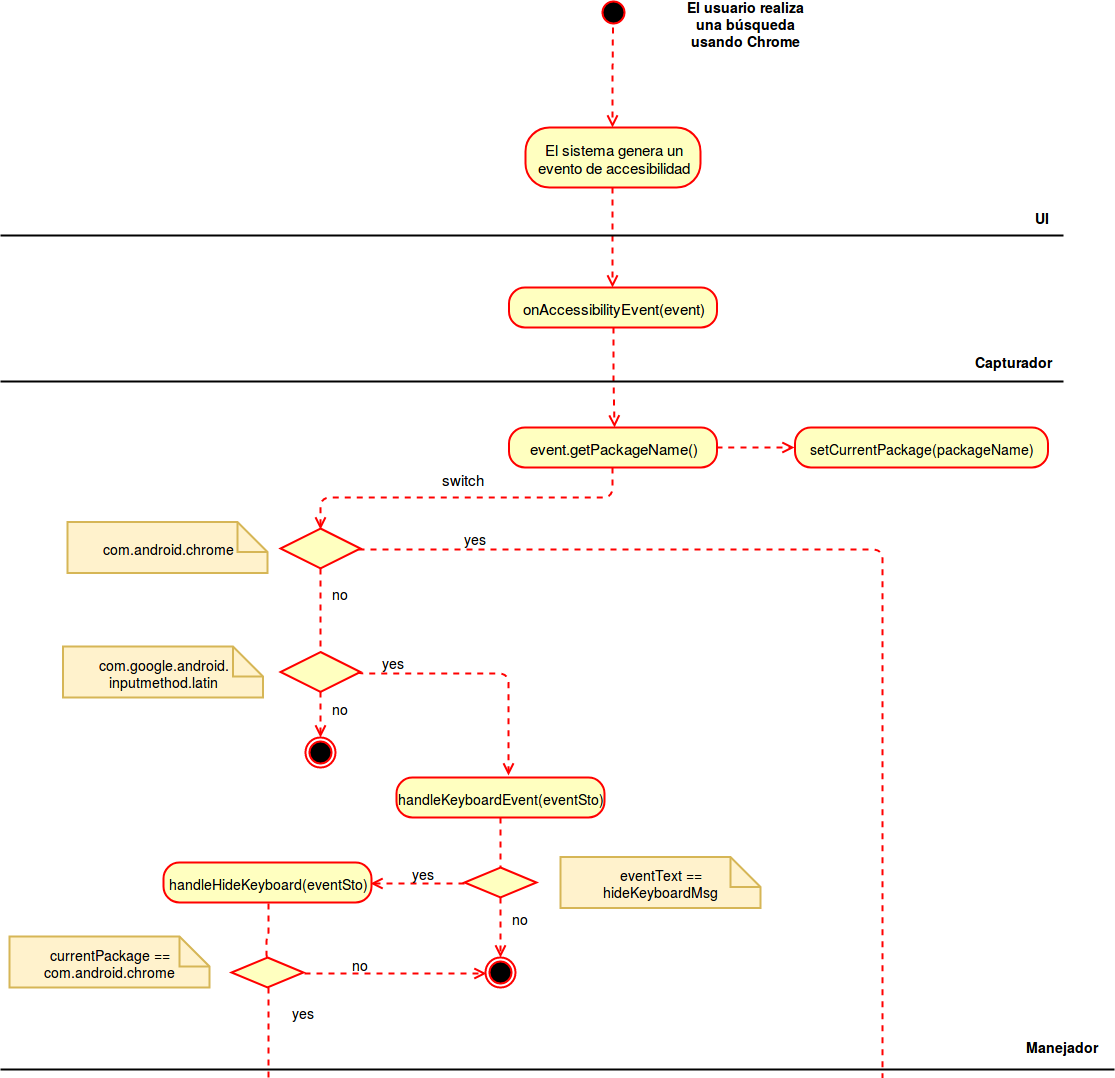
\includegraphics[scale=0.4]{pictures/activity/chromeActivityDiagram1.png}
	    	\caption{Diagrama de actividad de Chrome (1)}{Diagrama de actividad de Chrome (1)}
    	\label{fig:Diagrama de actividad Chrome (1)}
	\end{center}
\end{figure}
\end{landscape}
\begin{landscape}
\begin{figure}[htb]
	\begin{center}
     	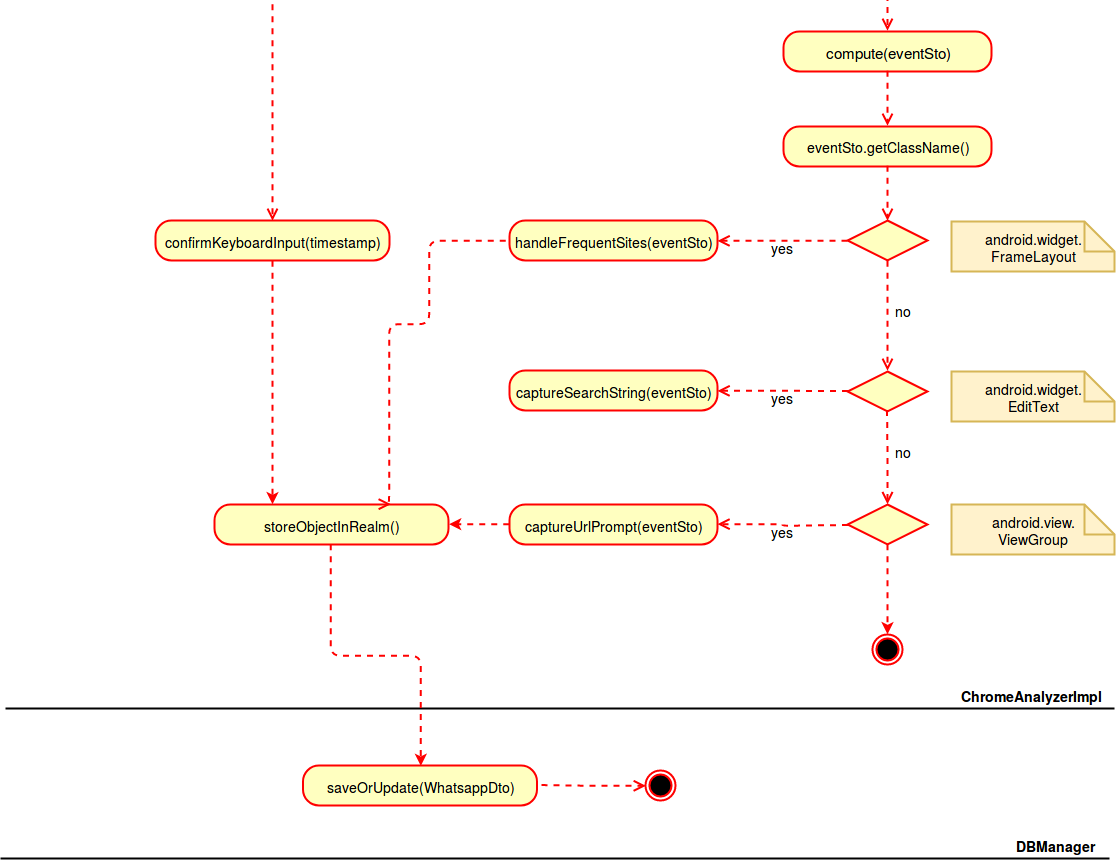
\includegraphics[scale=0.4]{pictures/activity/chromeActivityDiagram2.png}
	    	\caption{Diagrama de actividad de Chrome (2)}{Diagrama de actividad de Chrome (2)}
    	\label{fig:Diagrama de actividad Chrome (2)}
	\end{center}
\end{figure}
\end{landscape}
De nuevo, la actividad de análisis recae en su mayor parte en el método compute del ChromeAnalyzerImpl. Este compute se encarga, como se puede observar, de, en función del nombre de la clase del elemento de la ui asociado al evento, llamar a diversos métodos para construir el objeto donde alojaremos la información de la captura. 
\subsubsection{handleFrequentSites(eventSto)}
Nos ayuda a extraer del evento el texto asociado a la pulsación de un sitio frecuente. En primer lugar, se verifica que la cadena no sea vacía. Si esto es así, se instancia un nuevo objeto del tipo ChromeDto, se le añade el timestamp y el texto de búsqueda (propio texto del evento). 
\newline \newline 
Una vez hecho esto, se invoca al método storeObjectInRealm(), encargado de su persistencia. 
\subsubsection{captureSearchString(eventSto)}
Este método, en primer lugar verifica que la cadena de búsqueda sea válida. En concreto, verifica que su longitud es mayor a la unidad. Esto es así porque a veces y de forma aparentemente aleatoria, se generan eventos de accesibilidad que han conseguido superar todos los filtros de cada nivel hasta llegar aquí, pero su contenido es la primer letra de la búsqueda o url. 
\newline \newline 
Seguido de esto, se comprueba que el evento es del tipo \textit{text selection changed} y superado este filtro, se instancia un nuevo objeto del tipo ChromeDto, se le añade la marca horaria, cadena de búsqueda y se deja el objeto preparado para cuando llegue el evento de teclado responsable de confirmar la entrada de texto. 
\subsubsection{captureUrlPrompt(eventSto)}
Llamaremos a este método cuando el usuario presione sobre los sitios frecuentes, sugeridos por el propio Chrome. 
\newline \newline 
La primera tarea que debe realizar el método es extraer la url visitada del texto del evento, puesto que este texto en crudo contiene la propia url y además, concatenada, el título de la página con la primera letra en mayúsculas. 
\newline \newline 
Una vez obtenida la url visitada (se puede extraer recorriendo la cadena y buscando el carácter que está en mayúsculas), instanciamos un nuevo ChromeDto, le añadimos el timestamp, la cadena de búsqueda y persistimos en la base de datos. 
\newline \newline
De esta manera, podremos saber que páginas visita el usuario con su marca horaria. Los hábitos de navegación son un factor determinante a la hora de definir el perfil de usuario, puesto que una persona cuando busca en la web se refleja a sí misma, sus dudas, inquietudes y sus intereses. Cabe decir que en el proyecto se incluye también la captura de la barra de búsqueda de Google, por estar incluida en la mayoría de versiones de Android, y el navegador Firefox, al ser el segundo más asentado en el mercado. 
\section{Manual de usuario}
Una vez se haya instalado la aplicación y se ejecute por primera vez, lo primero que verá el usuario será una solicitud de permisos, que deberá aceptar si quiere que el servicio de localización funcione correctamente. De esta forma, tendremos la siguiente captura como primera pantalla, en caso de ser la primera ejecución. 
\begin{figure}[H]
	\begin{center}
     	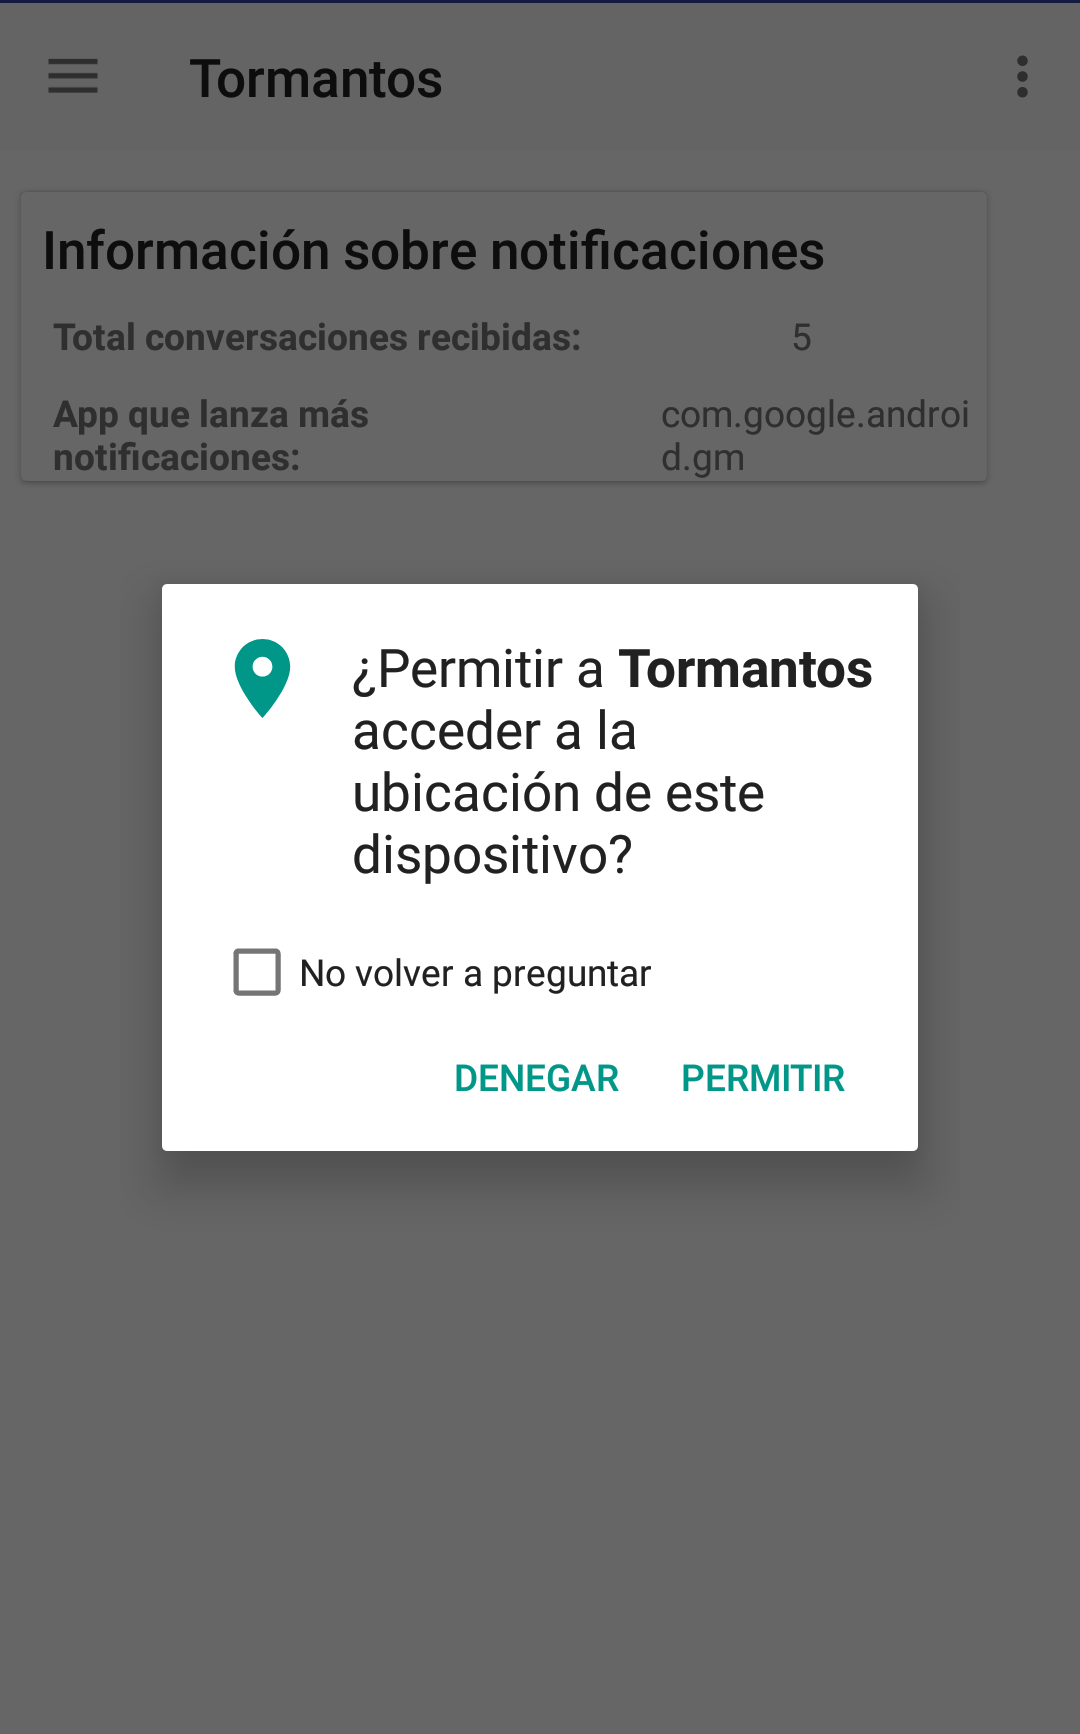
\includegraphics[scale=0.2]{pictures/capsapp/home3.png}
	    	\caption{Pantalla de la app en la primera ejecución}
    	\label{fig:Pantalla de la app en la primera ejecucion}
	\end{center}
\end{figure}
Una vez el usuario autorice el acceso a la ubicación, lo siguiente que se le muestra es una pantalla de bienvenida, donde se detalla el propósito de la app (siempre destinado a no desvelar el proceso de captura en segundo plano). Además, dado que la aplicación necesita tener activado el permiso de accesibilidad, si no se encuentra concedido, se mostrará un mensaje en rojo a modo de aviso. Este mensaje explica que para funcionar correctamente, el usuario necesita conceder, de forma explícita, estos permisos. 
\newline \newline 
Además, para mayor comodidad, se ofrece un botón de modo de \textit{shortcut} para ir directamente a esta opción de los ajustes. 
\begin{figure}[H]
	\begin{center}
     	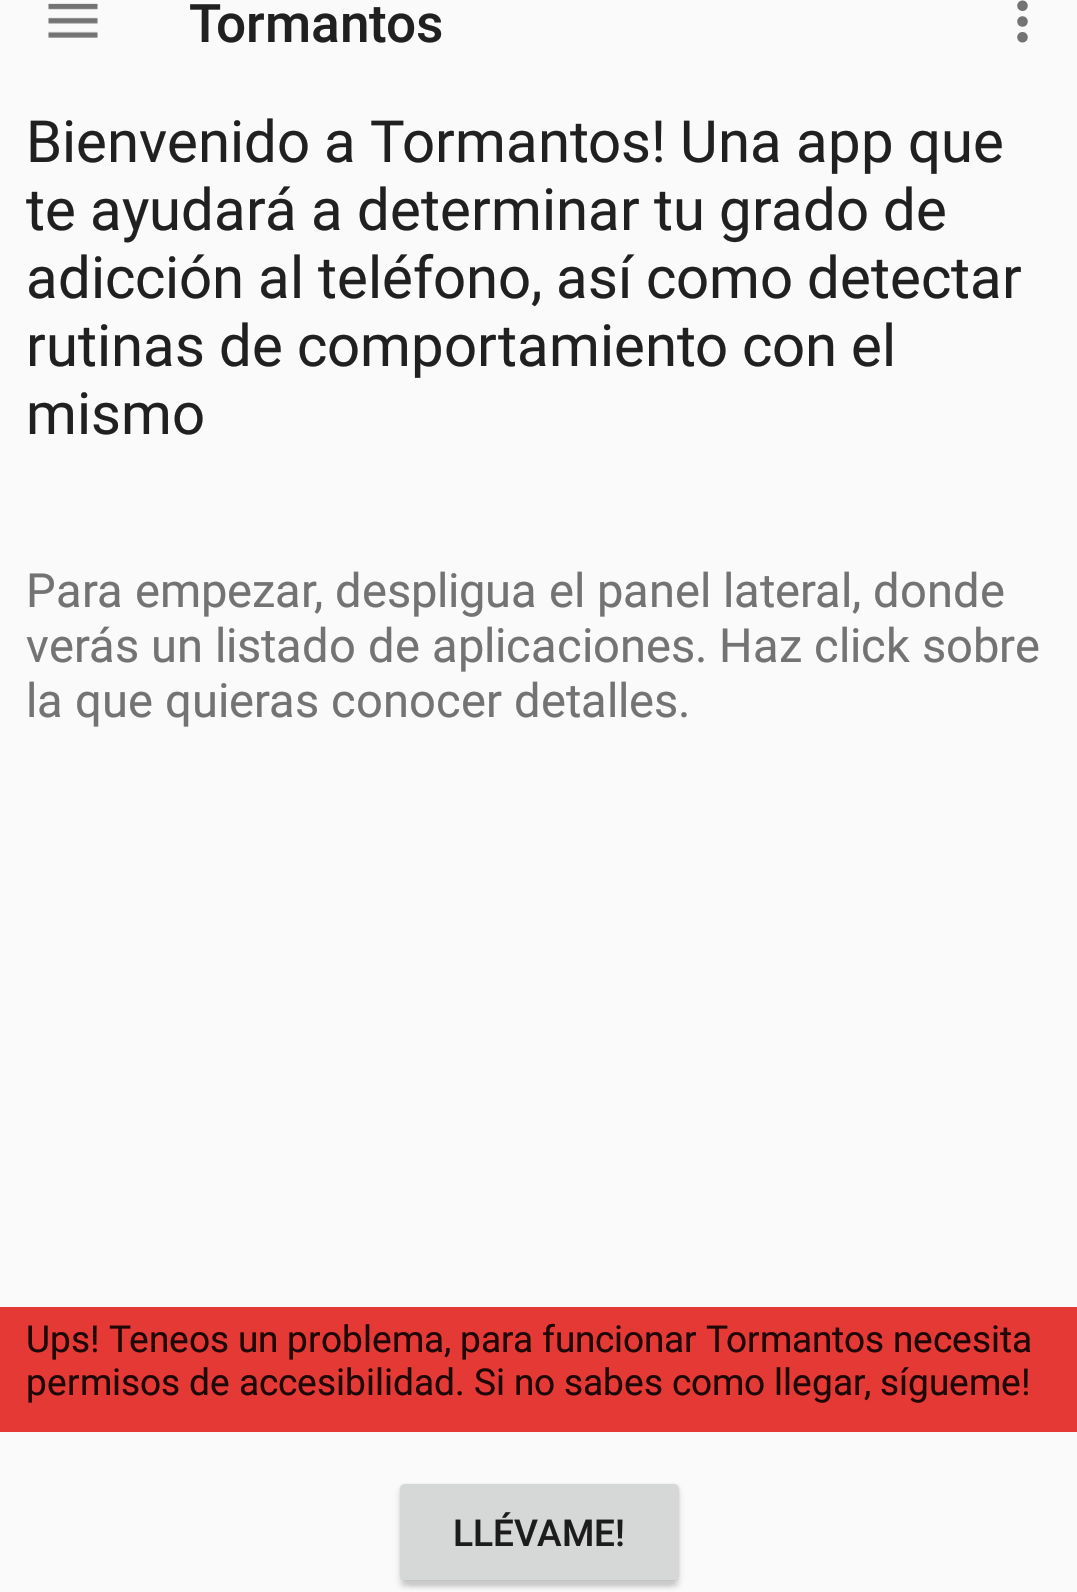
\includegraphics[scale=0.2]{pictures/capsapp/home1.png}
	    	\caption{Pantalla de bienvenida, mostrando el aviso de accesibilidad}
    	\label{fig:Pantalla de bienvenida, mostrando el aviso de accesibilidad}
	\end{center}
\end{figure}
Si el usuario pulsa sobre el botón que le ofrecemos, será redirigido a la siguiente pantalla, correspondiente a los ajustes de accesibilidad de la aplicación. En ella, deberá activar el toggle hasta llevarlo al estado \textit{activado}, tal y como figura en la siguiente imagen. 
\begin{figure}[H]
	\begin{center}
     	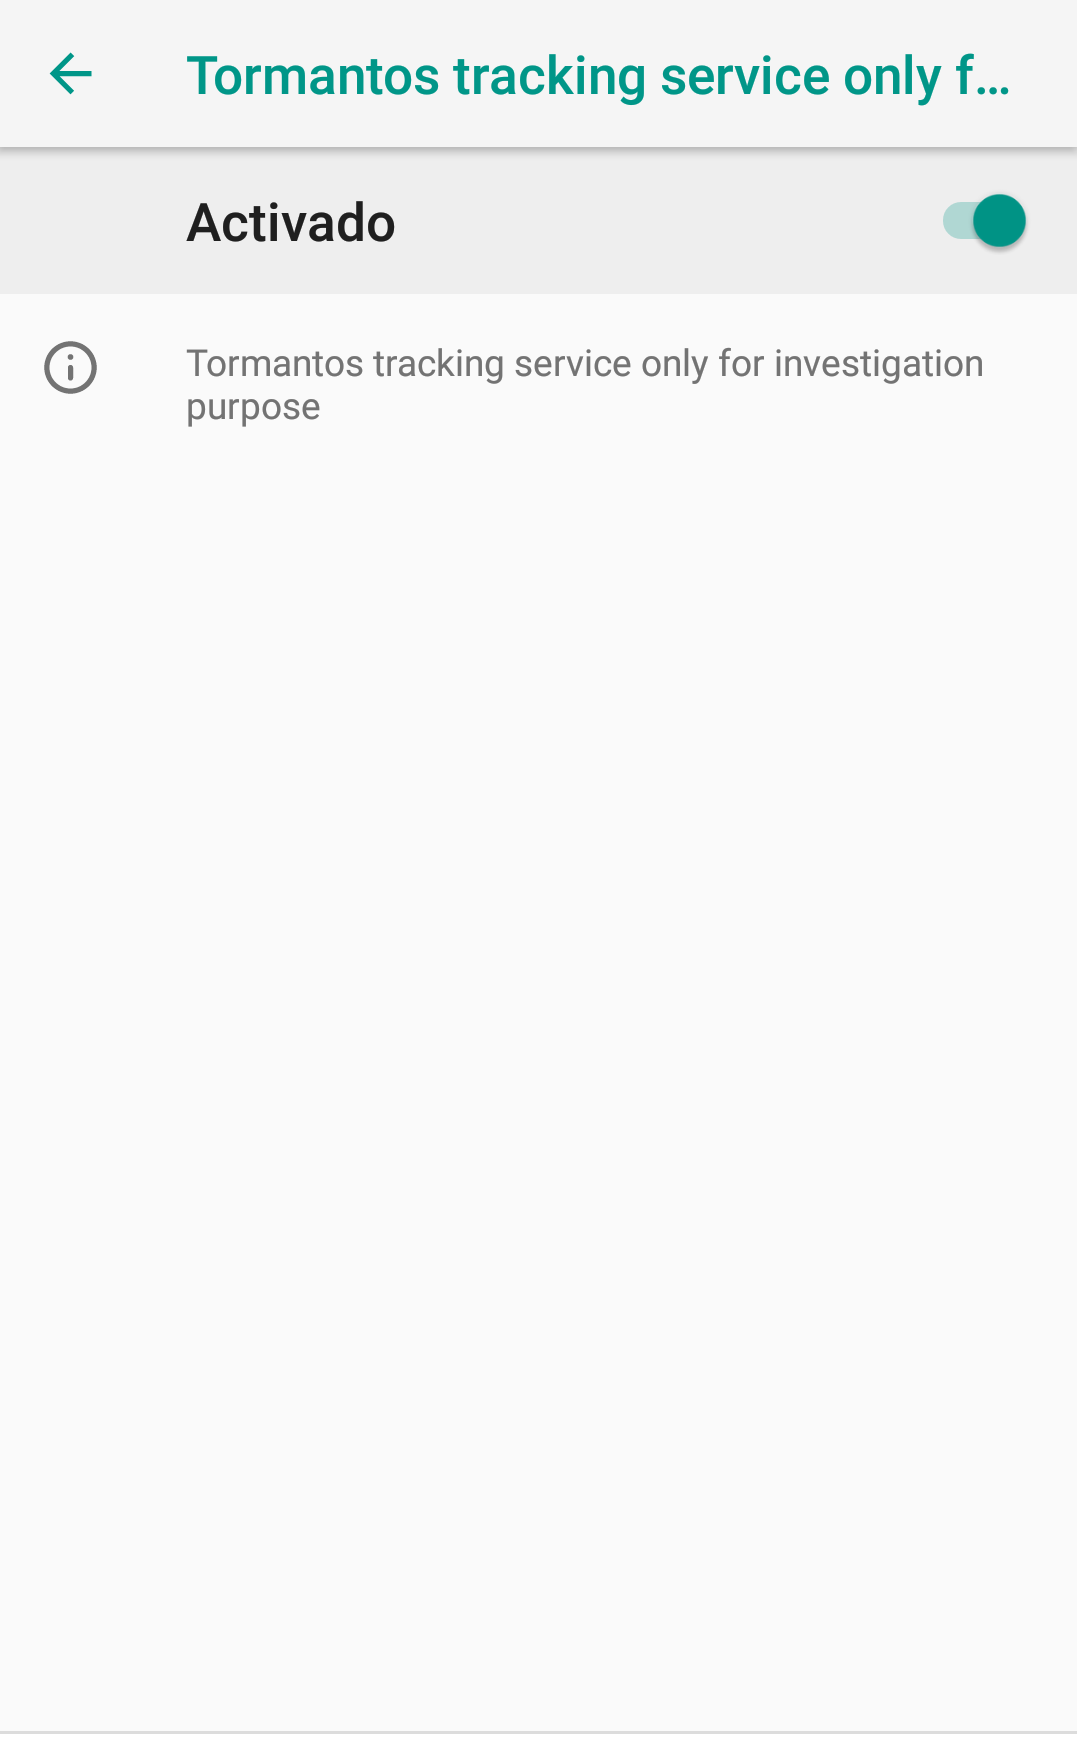
\includegraphics[scale=0.2]{pictures/capsapp/accessibility.png}
	    	\caption{Ajustes de accesibilidad de Tormantos}
    	\label{fig:Ajustes de accesibilidad de Tormantos}
	\end{center}
\end{figure}
Si volvemos a la aplicación, veremos que el estado de la pantalla ha cambiado, ya no muestra el aviso, por el contrario, se ofrece la pantalla de bienvenida de forma limpia y sin más elementos que el mensaje descriptivo. 
\begin{figure}[H]
	\begin{center}
     	\includegraphics[scale=0.2]{pictures/capsapp/home2.png}
	    	\caption{Pantalla de bienvenida sin el mensaje de aviso}
    	\label{fig:Pantalla de bienvenida sin el mensaje de aviso}
	\end{center}
\end{figure}
Observamos, en la esquina superior izquierda un icono, si lo pulsamos, lanzaremos la acción de despliegue del panel lateral, donde se encuentras las opciones de nuestra aplicación. 
\begin{figure}[H]
	\begin{center}
     	\includegraphics[scale=0.2]{pictures/capsapp/navigation.png}
	    	\caption{Navigation drawer de la aplicación desplegado}
    	\label{fig:Navigation drawer de la aplicacion desplegado}
	\end{center}
\end{figure}
En este nuevo menú lateral, observamos 4 categorías, a saber, Apps de comunicación, con la opción \textit{Comunicación}, Mensajería, con la opción \textbf{Mensajería instantánea}, Navegación con Web, con la opción \textit{Navegadores} y la última, información generada por el sistema, con la opción sistema. 
\newline \newline 
Si el usuario decide pulsar sobre alguna de estas opciones, se mostrará la siguiente información. 
\subsubsection{Comunicación}
Se muestra la siguiente pantalla. 
\begin{figure}[H]
	\begin{center}
     	\includegraphics[scale=0.2]{pictures/capsapp/navigation.png}
	    	\caption{Pantalla de comunicación}
    	\label{fig:Pantalla de comunicacion}
	\end{center}
\end{figure}
En ella, y en una vista de tarjetas, se muestran los detalles del uso del télefono, uso de mensajes SMS y uso de Gmail. 
\newline \newline 
En el uso del teléfono, nos encontramos, en primer lugar, un recuento del tiempo que ha empleado el usuario utilizando la aplicación de \textit{teléfono} de su disposito. En la siguiente línea, el número total de llamadas realizadas, y en la tercera y última, el nombre del contacto más habitual en estas llamadas. 
\newline \newline 
En el uso de mensajes SMS la información mostrada es similar, por un lado el recuento del tiempo de uso de la aplicación, el número total de mensajes enviados y el contacto habitual, destinatario de esos mensajes. 
\newline \newline 
Por último, en el uso de Gmail, de nuevo vemos el recuento del tiempo empleado usando la app de Gmail, los correos enviados y la dirección de destinatario habitual de dichos correos. 
\subsection{Mensajería instantánea}
Si avanzamos en los elementos del panel lateral, llegaremos a la siguiente pantalla, que nos muestra la información acerca del uso de las aplicaciones de mensajería instantánea, Whatsapp y Telegram. 
\begin{figure}[H]
	\begin{center}
     	\includegraphics[scale=0.2]{pictures/capsapp/messaging.png}
	    	\caption{Pantalla de comunicación}
    	\label{fig:Pantalla de comunicacion}
	\end{center}
\end{figure}
En primer lugar, nos encontramos con información sobre Whatsapp. Como viene siendo habitual, tenemos un recuento del tiempo pasado utilizando la aplicación, así como el número de conversaciones distintas en las que ha entrado el usuario. 
\newline \newline 
Seguidamente, vemos un recuento del total de mensajes enviados por el usuario en los distintos chats, así como el nombre del contacto habitual de estos mensajes. 
\newline \newline 
En el caso de Telegram, la información mostrada es más reducida, puesto que únicamente nos ofrece un recuento de los mensajes enviados utilizando este sistema de mensajería. 
\subsubsection{Navegación web} 
Nos encontramos en esta ocasión con una vista que nos aporta información sobre el uso dado a los navegadores Chrome y Firefox. 
\begin{figure}[H]
	\begin{center}
     	\includegraphics[scale=0.2]{pictures/capsapp/browsing.png}
	    	\caption{Pantalla de navegación web}
    	\label{fig:Pantalla de navegacion web}
	\end{center}
\end{figure}
En ambos casos la información mostrada es la misma. El ya habitual recuento del tiempo de uso, el total de páginas visitadas con cada aplicación y, para ambas, la página más visitada usando el navegador correspondiente. 
\subsubsection{Sistema} 
Llegamos así hasta la última pantalla, la información generada por el sistema.
\begin{figure}[H]
	\begin{center}
     	\includegraphics[scale=0.2]{pictures/capsapp/system.png}
	    	\caption{Pantalla de información del sistema}
    	\label{fig:Pantalla de informacion del sistema}
	\end{center}
\end{figure}
La única información que se muestra aquí es la referente a las notificaciones recibidas en el teléfono. Tenemos por un lado, el número total de notificaciones que han entrado en nuestro terminal, así como el nombre del paquete de la aplicación responsable del mayor número de ellas.  
\section{Bibliotecas de terceros}
\subsection{Realm}
Realm es una base de datos cuya implementación para Android nos ofrece una alternativa a SQLite, destactando por su rapidez y facilidad de uso. 

Se trata de una base de datos orientada a objetos, facilitando así el mapeo objeto relacional a través del código, incluyendo de esta manera las facilidades de un ORM de forma nativa. 
\newline \newline
Para añadirla su dependencia basta con añadir en el build gradle (Project): 
\begin{verbatim}
		classpath "io.realm:realm-gradle-plugin:5.1.0"
\end{verbatim}
En este caso se está usando exactamente la versión 5.1.0. Deberemos añadir en el build gradle (App): 
\begin{verbatim}
		apply plugin: 'realm-android'

\end{verbatim}
\section{Requisitos incumplidos}
Aún con todo el trabajo que ha llevado el desarrollo del proyecto, algunos requisitos se han quedado fuera, bien por falta de tiempo de implementación, bien por limitaciones técnicas de los propios servicios de accesibilidad. Veámos cuales son, agrupándolos por grupos. 
\subsection{Aplicaciones de comunicación}
\begin{itemize}
\item Dentro de la aplicación de Gmail, ha resultado imposible capturar el cuerpo del correo electrónico, al no generarse eventos de accesibilidad asociados a esta acción. 
\end{itemize}
\subsection{Aplicaciones de mensajería instantánea}
\begin{itemize}
\item Dentro de la aplicación de Telegram, no se ha podido registrar el nombre del interlocutor, al no generarse eventos de accesibilidad asociados a la acción de pulsar sobre una conversación. 
\end{itemize}
\subsection{Búsqueda en la web}
\begin{itemize}
\item Dentro de la aplicación de Búsqueda de Google, no se ha podido registrar la cadena de búsqueda, al no generarse eventos de accesibilidad asociados a esta acción. 
\end{itemize}
\subsection{Aplicaciones de redes sociales}
\begin{itemize}
\item No se ha implementado la captura de twitter ni facebook por falta de tiempo en la implementación. 
\end{itemize}
%~\ref{fig:Calculo IDLE-PC} este valor es calculado automáticamente por el programa, algo que no pasa en versiones anteriores de este, donde se calculan varios valores que se muestran al usuario para que este seleccione uno de ellos.
%\begin{figure}[h]
%\centering
%\caption[Calculo IDLE-PC]{Calculo IDLE-PC}
%\label{fig:Calculo IDLE-PC}
%\end{figure}
\subsubsection{Conclusión}
El desarrollo de la aplicación vemos que tiene dos partes claramente diferenciadas, por un lado el servicio de escucha en segundo, del que el usuario cuanto menos sepa mejor. Y por otro, la interfaz de la aplicación, que debe ofrecer algún pretexto para mantener al usuario informado sobre la información que recoge el sistema, aunque sólo sea una pequeña parte del conjunto. 
\newline \newline 
A través de esta interfaz de usuario, se pretende mostrar al mismo una aproximación de las rutinas que adquiere con el teléfono, así como, siendo lo más importante, el tiempo gastado en cada app. 
\newline \newline 
Es importante recalcar el hecho de que esta aplicación no necesita que el usuario interactúe directamente con ella, si no que sencillamente se trata de una ventana a los datos obtenidos hasta el momento de su consulta.
\newline \newline 
Por lo demás, el desarrollo del servicio de captura, en el afán de querer recabar el máximo número de datos de cada faceta de la vida del usuario, se ha vuelto un proceso ampliamente extendido en el tiempo. Para capturar una aplicación hay que estudiar sus puntos de entradas, cada flujo de interacción alternativo que puede tomar el usuario y una vez sacados los patrones, plasmarlos en el analizador. 
\newline \newline 
Aún así, el fruto del trabajo se antoja positivo, puesto que hemos conseguido capturar los datos del usuario en el uso de las aplicaciones más frecuentes en cada campo, lo cual, personalmente, y dejando a un lado la cuestión ética, considero una opción muy interesante. 

\chapter{Conclusiones y trabajos futuros}
Como conclusión personal, que extraigo después de haber investigado sobre las técnicas de recolección de datos, y habiendo implementado una herramienta para tal propósito, tengo cada vez más claro que la privacidad en el siglo XXI es una quimera. Además da igual cuanto te preocupes por ella, cualquier paso en falso en internet permite que las grandes compañías consigan tu información personal y no puedas evitar que se trafique con tus datos. No hablemos ya si usamos un smartphone, en cuyo caso estamos vendidos a Google, Apple, o la compañía que proceda. 
\newline \newline 
Además, me asusta un poco lo desconocido. Me explico, que los proveedores de servicios quieren nuestros dato creo que está asumido por parte de la sociedad. Pero lo realmente aterrador es hasta donde se llega en ámbitos que no son conocidos por el público, y me refiero a casos de espionaje entre gobiernos, industrial, etc. 
\newline \newline 
Si un estudiante ha podido desarrollar una aplicación que es capaz de leer los mensajes que escribes en Whatsapp, no quiero ni imaginar de lo que son capaces equipos con inversión y recursos dedicados a trabajar en ello 24 horas al día. Basta con aprovecharse de cualquier fallo de seguridad para saltarse las restricciones que, por su propia naturaleza, Android impone en su sistema, para lograr leer la pantalla del usuario. Y no sólo eso, si no las veces en las que los usuarios, sin darnos cuenta, autorizamos operaciones de este tipo, escondidas entre el lenguaje jurídico de los términos y condiciones de los servicios. 
\newline \newline 
Por mi parte, tiraré por el camino del medio y una vez terminado el trabajo, instalaré una versión de LineageOS con los servicios mínimos de Google para poder usar el GPS. No creo que valga de mucho, pero al menos para ponérselo un poco menos fácil que hasta ahora, que estamos regalando nuestros datos (aunque también es verdad que ellos nos regalan sus servicios... vaya!). 
\section{Trabajos futuros}
Dado que este trabajo se enmarca dentro de un trabajo de fin de máster, el próximo paso lógico será emplear los datos recogidos por la aplicación para su estudio. 
\newline 
\newline 
Este estudio deberá consistir en un proceso de \textit{machine learning} para lograr, en última instancia, la predicción de alteraciones en el comportamiento del usuario. Esto podrá llevarse a cabo gracias a los datos recogidos dentro de aplicaciones que forman parte del día a día del usuario. Además, y como se ha dejado claro, cubrimos todas las facetas del usuario. De esta manera no tendremos puntos ciegos en los que desconozcamos como se interactúa el usuario en un determinado campo. 
\newline 
\newline 
Además, si se quiere ir mas allá con el proceso de captura, el proyecto está abierto a modificaciones. Se ha documentado el funcionamiento del sistema de captura, el papel que juegan los eventos, sus campos, etc. Si se desea, añadir nueva funcionalidad es tan fácil como implementar la interfaz disponible, sin que esto se traduzca en un cambio estructural del código. Dejemos que el proyecto viva!. 

%%%%%%%%%%%%%%%%%%%%%%%%%%%%%%%%%%
%%%%%%%%%%% ANEXOS %%%%%%%%%%%%%%%
%%%%%%%%%%%%%%%%%%%%%%%%%%%%%%%%%%
%%\appendix
%%%\clearpage
%%\appendixpage
%%%\addappheadtotoc

%%%%%\chapter{Ejemplo de anexo}
%%%%%%Si no se desea incluir anexos, sólo hay que borrar este capítulo.
%%%%%\par



\pagebreak
%%%%%%%%%%%%%%%%%%%%%%%%%%%%%%%%%%
%%%%%%%%%% AL FINAL %%%%%%%%%%%%%%
%%%%%%%%%%%%%%%%%%%%%%%%%%%%%%%%%%
\thispagestyle{empty}
\pagestyle{empty}
%%%% https://en.wikibooks.org/wiki/LaTeX/Bibliography_Management
\bibliography{bib}

\bibliographystyle{plain}
\end{document}
%%%%%\section{Secciones}
%%%%%Las secciones se crean con \textit{section}. Las subsecciones y %%%%subsubsecciones con \textit{subsection} y \textit{subsubsection}, %%%%respectivamente. Si se desea que alguna subsección en concreto no salga %%%%en el índice se pueden usar los mismos comandos añadiéndoles un %%asterisco al final (\textit{subsection*} y \textit{subsubsection*}).
%%\par

%%%%%\subsection{una subsección}

%%%%%%\subsection{otra subsección}
%%%%%%Excepteur sint obcaecat cupiditat non proident, sunt in culpa qui %%%%%%officia deserunt mollit anim id est laborum.
%%%%%%\subsubsection{subsubsecciones}
%%%%%%¡Por defecto las subsubsecciones no aparecen en el índice! Este %%%%%%comportamiento se puede cambiar.

%%%%%%\section{Citas y referencias}
%%%%%Para citar un texto hay que incluirlo en el fichero %%%%\textit{LocalBibliography.bib} de esta plantilla. Una vez hecho se 
%%%%%puede referenciar usando el comando \textit{cite}~\cite{LaTeX_tutorials}.
%%%%Para referenciar imágenes, secciones o tablas se usa el %%%%comando~\textit{ref}. Por ejemplo~\ref{fig:logoEpcc}. Es importante %%%%haber añadido una etiqueta con el nombre correspondiente al emenento a %referenciar.
%%%%%\par
%%%%%%Para facilitar la lectura, cuando se insertan citas y referencias %%%%%%es conveniente insertar un caracter de espacio sin salto de línea %%%%%%%%\textit{\~} antes del comando de cita o referencia.


%%%%%%\section{Imágenes}
%%%%%%Las imágenes se insertan así:

%%%%\begin{figure}[H]
%%%%%\centering
%%%%%\includegraphics[width=0.6\textwidth]{pictures/logoEpcc.png}
%%%%%%\caption[Logo Epcc]{Logo Epcc.\\Fuente:http://www.unex.es/conoce-la-uex/centros/epcc/}
%%%%%%\label{fig:logoEpcc}
%%%%%%\end{figure}
